%! Author = prat
%! Date = 14/04/2020

% Preamble
\documentclass[
    %fontsize=12pt % The default document font size, options: 10pt, 11pt, 12pt
    english, % ngerman for German
    onehalfspacing, % Single line spacing, alternatives: onehalfspacing or doublespacing
    headsepline, % Uncomment to get a line under the header
    parskip, % Uncomment to add space between paragraphs
]{MastersDoctoralThesis} % The class file specifying the document structure

% Packages
\usepackage{lmodern}
\usepackage{scrextend}
\KOMAoption{fontsize}{12.5pt}
\usepackage[utf8]{inputenc}
\usepackage{mathtools}
\usepackage{textcomp}
\usepackage{float}
\usepackage{makeidx}
\usepackage[T1]{fontenc}
\usepackage{url}
\usepackage{todonotes}
\usepackage[all]{xy}
\usepackage{units}
\usepackage{enumerate}
\usepackage[hidelinks]{hyperref}
\usepackage[]{algorithm2e} %algorithm
\usepackage[langfont=roman,basic]{complexity}
\usepackage{amssymb, amsmath, amsthm, pict2e}
\usepackage{pdfsync}
\usepackage{rotating}
\usepackage{multirow}
\usepackage[normalem]{ulem}
\usepackage{cancel}
\usepackage{color}
\usepackage{pgf,tikz}
\usetikzlibrary{decorations.markings}
\usepackage{subcaption}
\usetikzlibrary{positioning}
\usetikzlibrary{decorations,arrows, graphs, quotes}
\usetikzlibrary{shapes.misc, positioning}
\usepgflibrary{decorations.pathreplacing}
\usetikzlibrary{arrows.meta}
\usetikzlibrary{arrows,automata}


\def\arr{\hbox{𝓇}}
\usepackage{environ}
\usepackage{csquotes}
\usepackage{amsmath}
\usepackage{natbib}
\makeatletter
\newsavebox{\measure@tikzpicture}
\NewEnviron{scaletikzpicturetowidth}[1]{%
    \def\tikz@width{#1}%
    \def\tikzscale{1}\begin{lrbox}{\measure@tikzpicture}%
                         \BODY
    \end{lrbox}%
    \pgfmathparse{#1/\wd\measure@tikzpicture}%
    \edef\tikzscale{\pgfmathresult}%
    \BODY
}
\def\ver{0.12} %size of a vertex

\tikzset{middlearrow/.style={
    decoration={markings,
    mark= at position 0.6 with {\arrow[scale=5]{#1}} ,
    },
    postaction={decorate}
}
}

\tikzset{Bullet/.style={fill=black,draw,color=#1,circle,minimum size=2pt,scale=0.9}}


%%%%%%%%%%%%%%%%  start macros  %%%%%%%%%%%%%%%%%%%%%%%%%%%%%%%%%
\let\emph\relax
\DeclareTextFontCommand{\emph}{\bfseries\em}
\newtheorem{theorem}{Theorem}
\theoremstyle{definition}
\newtheorem{defn}[theorem]{Definition}
\newtheorem{example}[theorem]{Example}
\theoremstyle{remark}
\newtheorem{remark}[theorem]{Remark}
\newtheorem{question}[theorem]{Question}
\theoremstyle{plain}
\newtheorem{lemma}[theorem]{Lemma}
\newtheorem{claim}[theorem]{Claim}
\newtheorem{obs}[theorem]{Observation}
\newtheorem{prop}[theorem]{Proposition}
\newtheorem{corollary}[theorem]{Corollary}
\newtheorem{conjecture}[theorem]{Conjecture}
\newtheorem{hyp}[theorem]{Hypothesis}
\newtheorem{alg}[theorem]{Algorithm}
\numberwithin{theorem}{section}
\newtheorem{proofpart}{Part}
\DeclarePairedDelimiter\ceil{\lceil}{\rceil}
\DeclarePairedDelimiter\floor{\lfloor}{\rfloor}

%%%%%%%%%%%%%%%%  end macros  %%%%%%%%%%%%%%%%%%%%%%%%%%%%%%%%%

%----------------------------------------------------------------------------------------
%	MARGIN SETTINGS
%----------------------------------------------------------------------------------------

\geometry{
    paper=a4paper, % Change to letterpaper for US letter
    inner=2.5cm, % Inner margin
    outer=3.8cm, % Outer margin
    bindingoffset=.5cm, % Binding offset
    top=1.5cm, % Top margin
    bottom=1.5cm, % Bottom margin
%showframe, % Uncomment to show how the type block is set on the page
}
%----------------------------------------------------------------------------------------
%	THESIS INFORMATION
%----------------------------------------------------------------------------------------

\thesistitle{Reconfiguration Problems} % Your thesis title, this is used in the title and abstract, print it elsewhere with \ttitle
\supervisor{Dr. Jean \textsc{Cardinal}} % Your supervisor's name, this is used in the title page, print it elsewhere with \supname
\examiner{} % Your examiner's name, this is not currently used anywhere in the template, print it elsewhere with \examname
\degree{} % Your degree name, this is used in the title page and abstract, print it elsewhere with \degreename
\author{Prateeba \textsc{Ruggoo}} % Your name, this is used in the title page and abstract, print it elsewhere with \authorname
\addresses{} % Your address, this is not currently used anywhere in the template, print it elsewhere with \addressname

\subject{PSPACE COMPLETE Problems} % Your subject area, this is not currently used anywhere in the template, print it elsewhere with \subjectname
\keywords{} % Keywords for your thesis, this is not currently used anywhere in the template, print it elsewhere with \keywordnames
\university{\href{https://www.ulb.be}{Université libre de Bruxelles}} % Your university's name and URL, this is used in the title page and abstract, print it elsewhere with \univname
\department{\href{https://www2.ulb.ac.be/facs/sciences/info}{Department of Computer Science}} % Your department's name and URL, this is used in the title page and abstract, print it elsewhere with \deptname
\group{\href{http://researchgroup.university.com}{}} % Your research group's name and URL, this is used in the title page, print it elsewhere with \groupname
\faculty{\href{http://faculty.university.com}{}} % Your faculty's name and URL, this is used in the title page and abstract, print it elsewhere with \facname

\AtBeginDocument{
    \hypersetup{pdftitle=\ttitle} % Set the PDF's title to your title
    \hypersetup{pdfauthor=\authorname} % Set the PDF's author to your name
    \hypersetup{pdfkeywords=\keywordnames} % Set the PDF's keywords to your keywords
}

% Document
\begin{document}
    \frontmatter % Use roman page numbering style (i, ii, iii, iv...) for the pre-content pages
    \pagestyle{plain} % Default to the plain heading style until the thesis style is called for the body content

%----------------------------------------------------------------------------------------
%	TITLE PAGE
%----------------------------------------------------------------------------------------

    \begin{titlepage}
        \begin{center}

            \vspace*{.06\textheight}
            {\scshape\LARGE \univname\par}\vspace{1.5cm} % University name
            \textsc{\Large Master Thesis}\\[0.5cm] % Thesis type

            \HRule \\[0.4cm] % Horizontal line
            {\huge \bfseries \ttitle\par}\vspace{0.4cm} % Thesis title
            \HRule \\[1.5cm] % Horizontal line

            \begin{minipage}[t]{0.4\textwidth}
                \begin{flushleft} \large
                \emph{Author:}\\
                \href{}{\authorname} % Author name - remove the \href bracket to remove the link
                \end{flushleft}
            \end{minipage}
            \begin{minipage}[t]{0.4\textwidth}
                \begin{flushright} \large
                \emph{Supervisor:} \\
                \href{}{\supname} % Supervisor name - remove the \href bracket to remove the link
                \end{flushright}
            \end{minipage}\\[3cm]

            \vfill
            \groupname  \deptname  % Research group name and department name

            \vfill

            {\large \today}\\[4cm] % Date
            %\includegraphics{Logo} % University/department logo - uncomment to place it

            \vfill
        \end{center}
    \end{titlepage}

%----------------------------------------------------------------------------------------
%	QUOTATION PAGE
%----------------------------------------------------------------------------------------

    \vspace*{0.2\textheight}

    \noindent\enquote{\itshape Understand well as I may, my comprehension can only be an infinitesimal fraction of all I want to understand.}\bigbreak

    \hfill Ada Lovelace

%----------------------------------------------------------------------------------------
%	ABSTRACT PAGE
%----------------------------------------------------------------------------------------

    \begin{abstract}
        \addchaptertocentry{\abstractname} % Add the abstract to the table of contents
        Reconfiguration problems arise when we wish to find a step-by-step transformation between two feasible solutions of a problem
        such that all intermediate results are also feasible. Recently, study about the solution space of reconfiguration problems
        defined as \textit{reconfiguration graph} sparked great interest. In this work, we focus on the structural questions
        (Is the reconfiguration graph connected?, Is there a path between a node $s$ and a node $t$ in the reconfiguration graph?).
        In the first half this thesis we analyse various aspects of the Constraint Logic framework, from the book “Games, Puzzles and Computation”
        by Hearn and Demaine which provides several problems that are often a convenient starting point for reductions in order tp prove
        $\PSPACE$-hardness and present an in-depth study of the alternative formulation of NCL, the sliding tokens problem.
        In the second half of this thesis, we analyse the complexity results around the boolean Satisfiability reconfiguration problems and
        investigate dichotomies/tricotomies that have been established and their applications. We also focus on complementing some
        recent $\PSPACE-$hardness proofs given in \cite{cardinal_reconfiguration_2018} concerning the $k$-move Subset sum reconfiguration problem.


    \end{abstract}

%----------------------------------------------------------------------------------------
%	ACKNOWLEDGEMENTS
%----------------------------------------------------------------------------------------

    \begin{acknowledgements}
        \addchaptertocentry{\acknowledgementname} % Add the acknowledgements to the table of contents
        First and foremost, my utmost gratitude to Prof. Jean cardinal, whose patience and encouragement I will never forget.
        And whose door was always open whenever I had questions concerning my research or whenever I was lost, I could always
        count on him for guidance. He consistently allowed this thesis to be my own work, but steered me in the right direction whenever
        he thought I needed it.

        I am also deeply indebted to my parents who have given me the opportunity of an education and support throughout my life.
        Finally, I must express my very profound gratitude to my partner for providing me with continuous encouragement
        and a sounding board when required. This accomplishment would not have been possible without them. Thank you.

        %I would like to thank my little kitten, Koi ni who brings me everyday joy \ldots
    \end{acknowledgements}

%----------------------------------------------------------------------------------------
%	LIST OF CONTENTS/FIGURES/TABLES PAGES
%----------------------------------------------------------------------------------------
    \hypersetup{linkcolor=black}
    \tableofcontents % Prints the main table of contents

%\listoffigures % Prints the list of figures

%\listoftables % Prints the list of tables

%----------------------------------------------------------------------------------------
%	DEDICATION
%----------------------------------------------------------------------------------------

    \dedicatory{Every challenging work needs self efforts as well as
                the support of those who are very close to our heart.
                My humble effort I dedicate to my sweet and loving


                Family $\&$ Partner


                Whose love, affection and encouragement made me able to
                complete this challenge,

                Along with all hard working and respected


                Teachers}

%----------------------------------------------------------------------------------------
%	THESIS CONTENT - CHAPTERSFor/Dedicated to/To my\ldots
%----------------------------------------------------------------------------------------

    \mainmatter % Begin numeric (1,2,3...) page numbering

    \pagestyle{thesis} % Return the page headers back to the "thesis" style

% Include the chapters of the thesis as separate files from the Chapters folder
\chapter{Introduction}
\label{ch:intro}
%Algorithmic graph theory is useful in modeling real-world problems, where the domain of the problem is modeled as a graph and the constraints on the solution
%define feasible solutions. For example, consider the problem of activating a number of routers subject to pairwise incompatibility constraints. Here, router
%compatibilities can be modeled as a graph and a feasible solution as an independent set. Traditionally, the real-world user
%first defines a problem instance and then uses an algorithm to find a feasible solution which she then ‘‘implements’’ in the
%real world. However, some real-world situations do not follow this simple paradigm and are more dynamic because they
%allow the solution to ‘‘evolve’’ over time. For example, consider the situation where a set of routers is already active but
%the operator has been instructed to use a different set of routers, which also form an independent set. To maintain network
%functionality, she can only switch one router at a time, but she has to make sure that there are always enough active routers
%(say, at least k) and that they are pairwise compatible. Thus, she would like to switch between the two configurations, while
%maintaining enough compatible routers at every intermediate step.
%In general, this type of situation gives rise to a reconfiguration framework

Reconfiguration problems are combinatorial problems in which we are given a collection of configurations, together with some
transformation rule(s) that allows us to change one configuration to another such that each intermediate solution remains satisfiable at all times.
A configuration can be the arrangement of puzzle pieces, the location of a robot with respect to obstacles in space, or the ordering of symbols to
form a string. Combinatorial reconfiguration problems ask the reachability between the two given satisfying solutions. The area of reconfiguration
considers both structural and algorithmic problems on the space of solutions, under various definitions of feasibility and adjacency.


The \textit{reconfiguration framework} is defined in terms of a source problem, an instance of the source problem, a definition of a feasible solution
and a definition of adjacency of feasible solutions. Viewing reconfiguration problems from a graph-theoretic perspective, the notion of a
\textit{reconfiguration graph} naturally arises. Let $G$ be a reconfiguration graph where the vertex set consists of all
possible configurations and two nodes are connected by an edge if the corresponding configurations can each be obtained from the other by the
application of a single transformation rule,\textit{a reconfiguration step}. Any path or walk in the reconfiguration graph corresponds to a
sequence of reconfiguration steps called a \textit{reconfiguration sequence}.

Interest in combinatorial reconfiguration begun with the Sliding blocks puzzles and steadily increased during the last decade. The reconfiguration framework has recently been applied in a number of settings,
including vertex coloring \cite{bonsma}, \cite{bonsma_cereceda}, \cite{cereceda}, list-edge coloring \cite{ito_reconfiguration_2009}, clique, set cover,
integer programming, matching, spanning tree, matroid bases \cite{DBLP:journals/tcs/ItoDHPSUU11}, block puzzles \cite{hearn_pspace-completeness_2004},
shortest path \cite{shortest_path}, independent set \cite{hearn_pspace-completeness_2004},\cite{DBLP:journals/tcs/ItoDHPSUU11}, \cite{kaminski_complexity_2012},
and satisfiability \cite{DBLP:journals/siamcomp/GopalanKMP09}.
Many problems in $\P$ have their reconfigurability problems in $\P$ as well, such as spanning tree, matching, and matroid problems in general. On the other hand,
the reconfigurability of independent set, set cover, and integer programming are $\PSPACE$-complete \cite{DBLP:journals/tcs/ItoDHPSUU11}. In general however, knowing
the complexity of a decision problem does not allow us to directly infer the complexity status of its reconfigurability problem(s). Several $\NP$-complete problems have
reconfigurability analogues that are in $\P$, for example the $3$-colorability problem \cite{DBLP:conf/iwoca/JohnsonCH08}. Alternatively, some problems in $\P$
have reconfigurability versions that are $\PSPACE$-complete, such as shortest paths \cite{DBLP:journals/corr/abs-1009-3217} or the problem of deciding whether
two $4$-colorings of a given bipartite or planar graph are reconfigurable \cite{bonsma}.


This thesis does not attempt to catalogue all research results that can be categorized as reconfiguration, but instead focuses on demonstrating the
main themes in the area (Satisfiability reconfiguration problems and Binary integer programming reconfiguration problems) and complement some
recent $\PSPACE-$hardness proof given in \cite{cardinal_reconfiguration_2018}. More precisely, we go over and detail the $\PSPACE-$completeness of
the following decision problems :
\begin{itemize}
    \item Given two subsets of a set $S$ of integers of integers with the same sum, can one subset be transformed into the other by adding or removing
    at most 3 elements of $S$ at a time, such that the intermediate subsets also have the same sum ?
    \item Given two points in $\{0,1\}^{n}$ contained in a polytope $P$ specified by a constant number of linear inequalities, is there a path in the
    $n-$hypercube connecting the two points and contained in $P$ ?
\end{itemize}

In the first half of this thesis, we study the Nondeterministic Constraint Logic of Computation introduced by Hearn and Demaine.
The NCL framework consists of different graph games ($i.e.$ problems) specific for every major complexity class, more specifically the class $\PSPACE$.
These graph games are created in order to facilitate the reduction to other games. Reviewing NCL as part of this thesis is fundamental since it has
been and still is the trigger for many $\PSPACE-$ hardness results in recreational mathematics.

The the second part of this thesis focuses on Satisfiability reconfiguration problems and Binary integer programming reconfiguration problems.
Finally, in Chapter 7 our conclusions are presented and some proposals for future work are made.



\chapter{Preliminaries}
\label{chap:preliminaries}
This chapter serves as a general introduction to some mathematical concepts that are of interest to us.
\section{Graph theory}

\subsection{Basic Notation}
Let $G$ be a simple, undirected graph with vertex set $V(G)$ and edge set $E(G)$. The \textit{neighborhood} of a vertex $v$ is denoted by
$N_{G}(v) = \{u | uv \in E(G)\}$. The \textit{degree} of a vertex $v \in G$, denoted by $deg_{G}(v)$, is $|N_{G}(v)|$. Then
$\Delta(G) = max_{v \in V(G)} deg_{G}(v)$ and $\delta(G) = min_{v \in V(G)} deg_{G}(v) $ is the maximum and minimum degree of $G$, respectively.
A subgraph of $G$ is a graph $G^{'}$ such that $V(G^{'}) \subseteq V(G)$ and $E(G^{'}) \subseteq E(G)$ (see Fig.~\ref{fig:subgraph}).

A \textit{walk} of length $l$ from $v_0$ to $v_l$ in $G$ is a vertex sequence $v_0, \dots ,v_{l}$, such that for all
$i \in \{0,\dots,l-1\}$, $v_{i}v_{i+1} \in E(G)$. It is a path if all vertices are distinct. A path from a vertex $u$ to a vertex $v$ is also
called a \textit{$uv-$path}. A graph $G$ is \textit{connected} if there is a path between every pair of vertices. The \textit{$k$-th power} of
a graph $G = (V,E)$ is the graph $G^{k}$ whose vertex set is $V$ and two distinct vertices $u,v$ are adjacent in $G^{k}$ if and only if the
shortest path distance between $u$ and $v$ in $G$ is at most $k$.

An \textit{independent set} of a graph $G$ is a vextex-subset of $G$ in which
no two vertices are adjacent. Given a set of elements $\{1,2,\dots,n\}$ (called the universe, denoted $\mathcal{U}$) and a
collection $\mathcal{S}$ of $m$ sets whose union equals the universe, an \textit{exact cover} is a sub-collection $\mathcal{S}^{*}$ of $\mathcal{S}$
such that each element in $\mathcal{U}$ is contained in exactly one subset in $\mathcal{S}^{*}$.
For an in-depth review of general graph theoretic definitions, the reader can refer to Diestel's textbook \cite{diestel_graph_2000}.
%%%%%%%%%%%%%%%%%%%%%%%%%%%%%%%%%%%%%%%%%%%%%%%% BEGINING OF A FIGURE %%%%%%%%%%%%%%%%%%%%%%%%%%%%%%%%%%%%%%%%%%%%%%%
\begin{figure} [H]
    \centering
    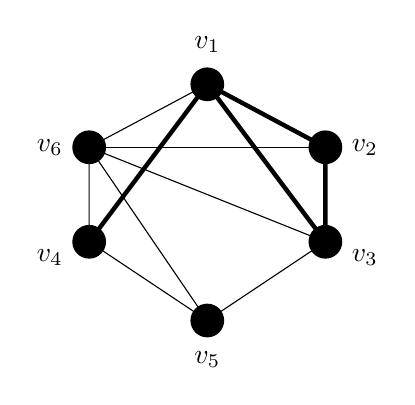
\begin{tikzpicture}
        \def\xa{1}
        \def\ya{5}
        %nodes
        \draw[thick, fill=black] (\xa,\ya) circle (0.2cm);         % v5
        \draw[thick, fill=black] (\xa+1.5,\ya+1) circle (0.2cm);   % v3
        \draw[thick, fill=black] (\xa+1.5,\ya+2.2) circle (0.2cm); % v2
        \draw[thick, fill=black] (\xa,\ya+3) circle (0.2cm);       % v1
        \draw[thick, fill=black] (\xa-1.5,\ya+2.2) circle (0.2cm); % v6
        \draw[thick, fill=black] (\xa-1.5,\ya+1) circle (0.2cm);   % v4
        %labels
        \node (1) at (\xa,\ya+3.5) {$v_1$};     % v1
        \node (2) at (\xa+2,\ya+2.2) {$v_2$};   % v2
        \node (3) at (\xa+2,\ya+0.8) {$v_3$};   % v3
        \node (5) at (\xa,\ya-0.5) {$v_5$};     % v5
        \node (4) at (\xa-2,\ya+0.8) {$v_4$};   % v4
        \node (6) at (\xa-2,\ya+2.2) {$v_6$};   % v6
        %edges
        \draw (\xa,\ya)--(\xa+1.5,\ya+1)--(\xa+1.5,\ya+2.2)--(\xa,\ya+3)--(\xa-1.5,\ya+2.2)--(\xa-1.5,\ya+1)--(\xa,\ya) ; % contour
        \draw (\xa,\ya)--(\xa-1.5,\ya+2.2) ;         % v5 - v6
        \draw (\xa+1.5,\ya+1)--(\xa-1.5,\ya+2.2) ;   % v3 - v6
        \draw (\xa+1.5,\ya+2.2)--(\xa-1.5,\ya+2.2) ; % v2 - v6
        \draw (\xa,\ya+3)--(\xa-1.5,\ya+1) ;         % v1 - v4
        \draw (\xa,\ya+3)--(\xa+1.5,\ya+1) ;         % v1 - v3
        % Hypergraph
        %edges
        \draw[ultra thick] (\xa,\ya+3)--(\xa+1.5,\ya+2.2)--(\xa+1.5,\ya+1)--(\xa,\ya+3) ; % contour
        \draw[ultra thick] (\xa,\ya+3)--(\xa-1.5,\ya+1) ;         % v1 - v4
    \end{tikzpicture}
    \caption{Graph $G^{'}$ (shown darker) is a subgraph of $G$.}
    \label{fig:subgraph}
\end{figure}
%%%%%%%%%%%%%%%%%%%%%%%%%%%%%%%%%%%%%%%%%%%%%%%% ENDING OF A FIGURE %%%%%%%%%%%%%%%%%%%%%%%%%%%%%%%%%%%%%%%%%%%%%%%

\subsection{Graph colouring}
In graph theory, a \textit{graph colouring} is a special case of \textit{graph labeling} as it is an assignment of labels traditionally
called "colours" to elements of a graph subject to certain constraints. In this work, the type of colourig that is of interest is
\textit{vertex colouring}. A \textit{proper vertex colouring} is a labeling of the graph’s vertices with colours such that no two adjacent
vertices have the same color.

A colouring using at most $k$ colours is called a \textit{(proper) $k$-colouring}.
A (proper) \textit{$k$-vertex-colouring} of a graph $G$ is a mapping $\phi$ from $V(G)$ to $\{1, 2, \dots, k\}$ (whose elements are called
\textit{colours})such that no two adjacent vertices receive the same colour, that is, $\phi(v) \neq \phi(v^{'})$ for all $v, v^{'} \in V(G)$
where $v \neq v^{'}$.
The \textit{chromatic number} of a graph $G$, denoted
$\chi{G}$, is the least number of distinct colours with which $G$ can be properly coloured. A graph that can be assigned a \textit{(proper) $k$-colouring}
is \textit{$k$-colorable}, and it is \textit{$k$-chromatic} if its chromatic number is exactly $k$. A subset of vertices assigned to the same colour
is called a \textit{colour class}, every such class forms an \textit{independent set}. Thus, a $k$-coloring is the same as a partition of the
vertex set into $k$ independent sets.


\section{Computational Complexity Theory} \label{sec:complexity}
Computer problems come in different varieties; some are easy, and some are hard. For example the sorting problem is an easy one compared to the
scheduling problem where say we have to find a schedule for the entire university to satisfy some reasonable constraints, such as that no two classes
take place in the same room at the same time. The scheduling problem seems to be much harder than the sorting problem.

In theoretical computer science, the theory of computation studies how efficiently a problem can be solved on a model of computation, using an
algorithm. A \textit{problem} or a \textit{language} is a set $L$ of strings of length at most $n$ over a finite alphabet $\Sigma$.
A \textit{decision problem} is a problem that can be posed as a YES/NO question. A string $s \in L$ is a yes instance of $L$ and a string $s \notin L$ is
a no-instance of $L$. An \textit{algorithm} is an unambiguous procedure of how to solve a class of problems.

The model of computation focused on in standard complexity theory is the \textit{Turing Machine}. It uses an unlimited tape as its unlimited memory
and has a tape head that can write and read symbols and move along the tape. A Turing Machine can be viewed as an automaton, following simple rules
to change states, with an aim to end in an accepting or a rejecting state. Two critical ressources for the Turing Machine are \textit{time} which is
the number of steps it requires to reach an accepting or a rejecting state and \textit{space} being the amount of information that needs to be
remembered throughout the computation.

A Turing Machine that can choose which moves to take in order to reach an accepting state is known as a \textit{Nondeterministic Turing Machine}
contrary to a \textit{Deterministic Turing Machine} (see Fig.~\ref{fig:computations}).
%%%%%%%%%%%%%%%%%%%%%%%%%%%%%%%%%%%%%%%%%%%%%%%% BEGINING OF A FIGURE %%%%%%%%%%%%%%%%%%%%%%%%%%%%%%%%%%%%%%%%%%%%%%%
\begin{figure}
  \begin{subfigure}[b]{0.4\textwidth}
    \centering
      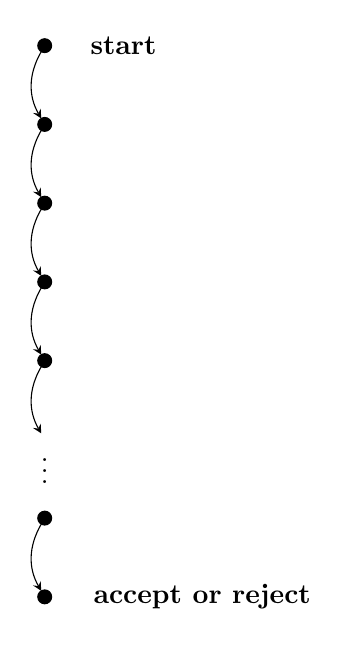
\begin{tikzpicture}[
          auto, >=stealth, node distance=0.0ex and 2em,
          pil/.style={->},
          dot/.style={circle, draw=black, fill=black, minimum size=#1, inner sep=0pt, outer sep=0pt} ]
          %nodes
          \node[dot=5pt, color=black] (start) at (0,10) {};   % start
          \node (s) at (1,10) {\textbf{start}};               % Label start
          \node[dot=5pt, color=black] (v1) at (0,9) {};       % v1
          \node[dot=5pt, color=black] (v2) at (0,8) {};       % v2
          \node[dot=5pt, color=black] (v3) at (0,7) {};       % v3
          \node[dot=5pt, color=black] (v4) at (0,6) {};       % v4
          \node[dot=5pt, color=white] (v5) at (0,5) {};       % v5
          \node (vdots) at (0,4.7) {$\vdots$};
          \node[dot=5pt, color=black] (v6) at (0,4) {};       % v6
          \node[dot=5pt, color=black] (v7) at (0,3) {};       % v7
          \node (a) at (2,3) {\textbf{accept or reject}};  % Label start
          %edges
          \path[pil] (start) edge[bend right] (v1);
          \path[pil] (v1) edge[bend right] (v2);
          \path[pil] (v2) edge[bend right] (v3);
          \path[pil] (v3) edge[bend right] (v4);
          \path[pil] (v4) edge[bend right] (v5);
          \path[pil] (v6) edge[bend right] (v7);
      \end{tikzpicture}
      \caption{Deterministic computation.}
      \label{fig:deterministic}
  \end{subfigure}
  \hspace{5em} % vertical space
  \begin{subfigure}[b]{0.4\textwidth}
    \centering
      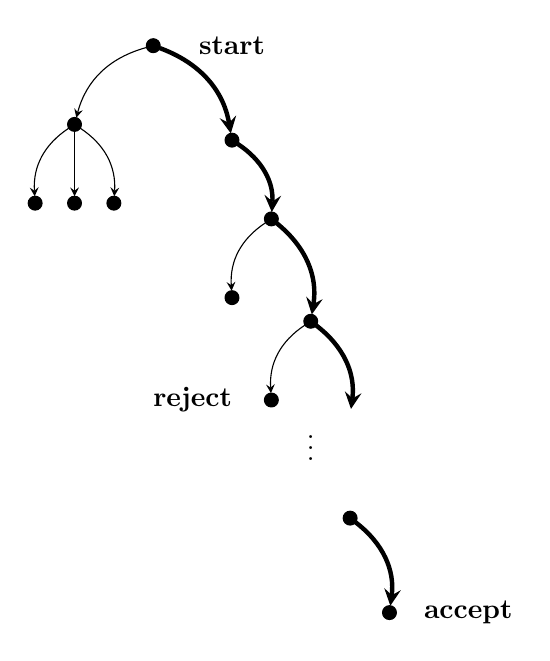
\begin{tikzpicture}[
          auto, >=stealth, node distance=0.0ex and 2em,
          pil/.style={->},
          dot/.style={circle, draw=black, fill=black, minimum size=#1, inner sep=0pt, outer sep=0pt} ]
        %nodes
        \node[dot=5pt, color=black] (start) at (0,10) {};       % start
        \node (s) at (1,10) {\textbf{start}};                   % Label start
        \node[dot=5pt, color=black] (v1) at (-1,9) {};          % v1
        \node[dot=5pt, color=black] (v2) at (1,8.8) {};         % v2
        \node[dot=5pt, color=black] (v3) at (-1.5,8) {};        % v3
        \node[dot=5pt, color=black] (v4) at (-1,8) {};          % v4
        \node[dot=5pt, color=black] (v5) at (-0.5,8) {};        % v5
        \node[dot=5pt, color=black] (v6) at (1.5,7.8) {};       % v6
        \node[dot=5pt, color=black] (v7) at (1,6.8) {};         % v7
        \node[dot=5pt, color=black] (v8) at (2,6.5) {};         % v8
        \node[dot=5pt, color=black] (v9) at (1.5,5.5) {};       % v9
        \node[dot=5pt, color=white] (v10) at (2.5,5.3) {};      % v10
        \node (vdots) at (2,5) {$\vdots$};
        \node[dot=5pt, color=black] (v11) at (2.5,4) {};        % v11
        \node[dot=5pt, color=black] (v12) at (3,2.8) {};        % v12
        \node (a) at (0.5,5.5) {\textbf{reject}};            % Label reject
        \node (b) at (4,2.8) {\textbf{accept}};              % Label accept
        %edges
        \path[pil] (start) edge[bend right] (v1);
        \path[pil, ultra thick] (start) edge[bend left] (v2);
        \path[pil] (v1) edge[bend right] (v3);
        \path[pil] (v1) edge (v4);
        \path[pil] (v1) edge[bend left] (v5);
        \path[pil, ultra thick] (v2) edge[bend left] (v6);
        \path[pil] (v6) edge[bend right] (v7);
        \path[pil, ultra thick] (v6) edge[bend left] (v8);
        \path[pil] (v8) edge[bend right] (v9);
        \path[pil, ultra thick] (v8) edge[bend left] (v10);
        \path[pil, ultra thick] (v11) edge[bend left] (v12);
      \end{tikzpicture}
      \caption{Nondeterministic computation.}
      \label{fig:nondeterministic}
  \end{subfigure}
  \caption{Deterministic and Nondeterministic computations with an accepting branch.}
  \label{fig:computations}
\end{figure}
%%%%%%%%%%%%%%%%%%%%%%%%%%%%%%%%%%%%%%%%%%%%%%%% ENDING OF A FIGURE %%%%%%%%%%%%%%%%%%%%%%%%%%%%%%%%%%%%%%%%%%%%%%%

\subsection{Computational Complexity Classes}\label{subsec:computational-complexity-classes}
Computational complexity theory contemplates not solely the solvability of a problem but also the resources required to solve computational problems.
It is divided in two branches: \textit{Time} complexity and \textit{Space} complexity as mentioned earlier. In this work, we give an informal
description of the classical complexity classes generally encountered. The interested reader can find full details and formal definitions in the
excellent textbook of Sipser \cite{sipserIntroductionTheoryComputation2006}. The following section describes the different computational complexity
classes in which different decision problems fits.

In general, these complexity classes study how the critical ressources (\textit{time} and \textit{space}) grows in terms if the input size.
For decision problems, the input is the description of the problem and its size measured as bits of information.

\subsubsection{Time complexity classes}
We start by characterizing in terms of time. The class $\P$ consists of all problems solvable in polynomial time, that is, all problems solved by
some algorithm in time that is at most linear, quadratic, cubic, or similar in the input size. If $n$ represents the input size, a general polynomial
might look like $5n^{4} + 3n^{2} + 10n - 1$.
Similarly, the class $\EXP$ consists of all problems solvable in exponential time:
$2^{n}, 5^{n}, 2^{n^{2}}$ or in general $2^{p(n)}$ where $p(n)$ is some polynomial. Note that $\EXP$ contains easier problems too, in particular,
all of $\P$.

\subsubsection{Space complexity classes}
On the other hand, the class $\PSPACE$ consists of all problems solvable in polynomial space. This class is the analog of $\P$ but measuring space
instead of time. Similarly, $\EXPSPACE$ consists of all problems solvable in exponential space.

Time and space complexity classes are related in the following way: An optimal algorithm never uses more space than time.
Thus, every problem in $\P$ is also in $\PSPACE$. Also, any (deterministic) algorithm that uses $s$ space can never use more than
exponential-in-$s$ time without repeating a position. Thus, every problem in $\PSPACE$ is also in $\EXP$.

\subsubsection{Nondeterminism}
Next, we consider allowing nondeterminism in order to solve a problem. A nondeterministic algorithm can at any computation step, proceed with
various possibilities (see Fig.~\ref{fig:nondeterministic}). A nondeterministic algorithm can be thought of as an extremly lucky: whenever it needs
to make a decision, it by defintion makes the correct choice. The class $\NP$ consists of all problems that can be solved in polynomial time by such a
nondeterministic algorithm. Similarly, we can define $\NPSPACE$ for the nondeterministic analog of $\PSPACE$, and $\NEXP$ for $\EXP$.

\subsubsection{Completeness}
For each complexity class $X$, we call a problem $X$-hard if it is about as hard as every problem in $X$. (Here, we ignore polynomial factors in the
difficulty.) We call a problem $X$-complete if it is both $X$-hard and in $X$. Thus, for example, $\NP$-complete problems are among the hardest problems
in $\NP$, so they must not be in any strictly easier complexity class. Whether $\P = \NP$ is of course a major open problem, but assuming they are even
slightly different, $\NP$-complete problems are not in $\P$. Thus, when classifying a problem into a particular complexity class, showing that the problem
is amongst the hardest problems in a certain complexity class eliminates any doubt of whether the latter belongs in a lower complexity class.
One technique of doing so is by \textit{reduction}.

\paragraph{Reducibility}
By taking a known $X$-complete problem $(B)$ and showing that solving the problem in which we are interested $(A)$ is at least as hard as solving $B$,
we can conclude that $A$ is $X$-hard. We usually do this by showing a way to transform problem $B$ into problem $A$.
\begin{defn}
A function $f : \Sigma^{*} \rightarrow \Sigma^{*}$ is a computable function if on every input $w$, some Turing machine $M$ halts with just $f(w)$ on its tape.
\end{defn}

\begin{defn}
Given two languages $A$ and $B$, $B$ is reducible to $A$ written $B \leq_{p} A$ if there is a computable function $f : \Sigma^{*} \rightarrow \Sigma^{*}$, where for
every $w, w \in B \Longleftrightarrow f(w) \in B$. The function $f$ is called the reduction of $B$ to $A$.
\end{defn}

\subsubsection{Relationship of Complexity Classes} \cite{hearn_demaine_ncl_book}
So far we have that $\P \subseteq \PSPACE \subseteq \EXP$. $\PSPACE = \NPSPACE$ follows from the celebrated result of Savitch \cite{savitch_relationships_1970}.
Concerning nondeterminism, a nondeterministic computation is at least as powerful as regular deterministic computation, so, for example, every problem
in $\P$ is also in $\NP$. On the other hand, nondeterministic computation can be simulated by trying both choices of each decision in turn, which
takes exponentially more time, but about the same amount of space. Thus, for example, every problem in $\NP$ is also in $\PSPACE$. Summing all
together, we can conclude that :
\begin{center}
  $\P \subseteq \NP \subseteq \PSPACE = \NPSPACE \subseteq \EXP \subseteq \NEXP \subseteq \EXPSPACE$
\end{center}
All of the containments are believed to be strict, but beyond the above relations, the only strict containment known among those
classes is $\P  \subsetneq \EXP$. Whether $\P = NP$ is the most famous unresolved question in Computational Complexity Theory.


\section{Reconfiguration Graph}
Viewing Reconfiguration problems from a graph-theoretic perspective, the notion of a \textit{reconfiguration graph} naturally arises.
Let $G = (V, E)$ be a reconfiguration graph where $V(G)$ is the vertex set consisting of all possible configurations and two nodes are
connected by an edge if the corresponding configurations can each be obtained from the other by the application of a single transformation rule,
\textit{a reconfiguration step}. Any path or walk in the reconfiguration graph corresponds to a sequence of reconfiguration steps called a
\textit{reconfiguration sequence}. Although the terminology concerning reconfiguration problems has not yet stabilized in the litterature those are
the terms that will be used throughout this work.


\section{Set theory}
The \textit{symmetric difference} of two sets $A$ and $B$ are elements in $A$ or $B$, but not in both $A$ and $B$ and written as
$A \triangle B$.

\chapter{The Nondeterministic Constraint Logic (NCL)} \label{chap:NCL}
In this Chapter, the Nondeterministic Constraint Logic model of computation is presented. This framework developped by Demaine and Hearn is
motivated by the Sliding-block puzzles \cite{hordern_sliding_1986}. The main result of \cite{hearn_pspace-completeness_2004} introduces the new
nondeterministic model of computation based on reversing edge directions in weighted directed graphs with minimum in-flow constraints on vertices.
This model, referred to as Nondeterministic Constraint Logic, or NCL, is shown to have the same computational power as a space-bounded Turing machine.

Several decision problems surrounding the NCL framework are proved to be $\PSPACE$-complete \cite{hearn_pspace-completeness_2004}. These decision problems are then used to prove the
$\PSPACE$-completeness of well-known Sliding-block puzzles such as Rush Hour and Sokoban \cite{hearn_demaine_ncl_book}. Demaine and Hearn argue that NCL can be considered as a
model of computation in its own right instead of just a set of decision problems. Thus, proving a problem to be $\PSPACE$-hard in the NCL
framework simply requires the construction of a couple of gadgets that can be connected together.
In the last section of \cite{hearn_pspace-completeness_2004} gives an interesting equivalent formulation of NCL in terms of sliding tokens along
graph edges. This latter formulation will be the focus of sections \ref{sec:sliding_tokens} and \ref{sec:labelled_sliding_token} to prove that
the Sliding token problem and labelled variant of the sliding token problem are $\PSPACE$-complete (theorems \ref{theorem:ncl_sliding_token}
and \ref{theorem:labelled_sliding} respectively).

\textit{Roadmap.} Section \ref{sec:formalism} describes the constraint logic using a graph formulation.
Section \ref{sec:contraint_graph} gives an overview of AND/OR constraint graphs which is the primary formulation used in the NCL framework.
Section \ref{sec:ncl_results} present some complexity results of decision problems stemming from the constraint logic framework.
In section \ref{sec:sliding_tokens} we detail the $\PSPACE$-completeness proof of the sliding token problem using the alternative
formulation of NCL (theorem \ref{theorem:ncl_sliding_token}). Lastly, in section \ref{sec:labelled_sliding_token} the hardness proof of the
labelled variant of the sliding token problem is given.

\section{Graph Formulation}\label{sec:formalism}
An NCL machine consists of a \textit{constraint graph}, $G = (V,E)$ that we can think of as our computation model.
Let $G$ be a $3$-regular graph with edge weights $ \in \{1, 2\}$. An edge is then called \textit{red} or \textit{blue}, respectively.
Each vertex has a nonnegative \textit{minimum inflow} which is the sum of the weights on inward-directed edges. A \textit{legal configuration}
is an assignment of an \textit{orientation(direction)} to each edge such that for every vertex $v$ of $G$, the sum of weights of inward-directed
edges of $v$ is at least $2$. A \textit{legal move} is the reversal of a single edge that results in another legal configuration.


\section{AND/OR Constraint Graphs} \label{sec:contraint_graph}
As part of the constraint logic framework,  Hearn and Demaine provided a restricted variant of Nondeterministic Constraint Logic (restricted NCL),
in which the constraint graph $G$ is planar, $3$-regular, uses only weights $ \in \{1,2\}$ and the graph is constructed from only two specific vertex
types ($AND$ and $OR$ vertices). A vertex $v$ of $G$ is an \textit{AND vertex} if exactly one incident edge has weight $2$ (Figure \ref{fig:and_vertex}) and
a vertex $v$ of $G$ is an \textit{OR vertex} if all the incident edges have weight $2$ (Figure \ref{fig:or_vertex}). Thus, a graph
$G$ is an \textit{AND/OR constraint graph} if it consists of only $AND$ and $OR$ vertices.

%%%%%%%%%%%%%%%%%%%%%%%%%%%%%% BEGINING OF A FIGURE : AND and OR vertex of constraint graph %%%%%%%%%%%%%%%%%%%%%%%%%%%%%
\begin{figure}[H]
  \begin{subfigure}[b]{0.4\textwidth}
    \centering
      \begin{scaletikzpicturetowidth}{\textwidth}
        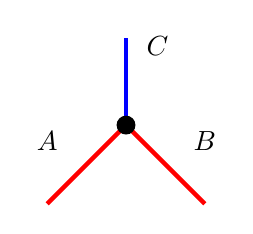
\begin{tikzpicture}
          \def\xa{0}     % AND
          \def\ya{0}
          %labels
          \node (1) at (\xa+0.4,\ya+1) {$C$};
          \node (2) at (\xa+1,\ya-0.2) {$B$};
          \node (2) at (\xa-1,\ya-0.2) {$A$};
          % f_1 arrows
          \draw[ultra thick, -, blue] (\xa, \ya) -- (\xa, \ya+1.1);
          \draw[ultra thick, -, red] (\xa, \ya) -- (\xa+1, \ya-1);
          \draw[ultra thick, -, red] (\xa, \ya) -- (\xa-1, \ya-1);
          % Nodes fill
          \path[fill] (\xa,\ya) circle (\ver);
        \end{tikzpicture}
      \end{scaletikzpicturetowidth}
      \caption{And vertex. Edge $C$ may be directed outward if and only if edges $A$ and $B$ are both directed inward.}
      \label{fig:and_vertex}
  \end{subfigure}
  \hspace{5em} % vertical space
  \begin{subfigure}[b]{0.4\textwidth}
    \centering
    \begin{scaletikzpicturetowidth}{\textwidth}
      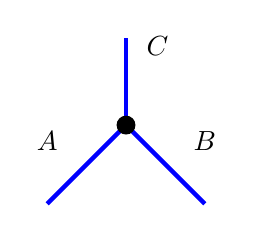
\begin{tikzpicture}
        \def\xb{5} % OR
        \def\yb{0}
        %labels
        \node (1) at (\xb+0.4,\yb+1) {$C$};
        \node (2) at (\xb+1,\yb-0.2) {$B$};
        \node (2) at (\xb-1,\yb-0.2) {$A$};
        % f_2 arrows
        \draw[ultra thick, -, blue] (\xb, \yb) --(\xb, \yb+1.1);
        \draw[ultra thick, -, blue] (\xb, \yb) --(\xb+1, \yb-1);
        \draw[ultra thick, -, blue] (\xb, \yb) --(\xb-1, \yb-1);
        % Nodes fill
        \path[fill] (\xb,\yb) circle (\ver);     % OR
      \end{tikzpicture}
    \end{scaletikzpicturetowidth}
    \caption{Or vertex. Edge $C$ may be directed outward if and only if either edge $A$ or edge $B$ is directed inward.}
    \label{fig:or_vertex}
  \end{subfigure}
  \caption{And and Or vertices. Red edges have weight $1$, blue edges have weight $2$, and all vertices have a minimum in-flow constraint of $2$.}
  \label{fig:and_or_vertices}
\end{figure}
%%%%%%%%%%%%%%%%%%%%%%%%%%%%%%%%%%%%%%%% ENDING OF A FIGURE %%%%%%%%%%%%%%%%%%%%%%%%%%%%%%%%%

\section{NCL Results} \label{sec:ncl_results}
This section compiles the important complexity results linked to NCL. A first fundamental decision problem that arises in the NCL framework
is about the satisfiability of a given constraint graph $G$. It is defined as follows :
\begin{flushleft}
  CONSTRAINT GRAPH SATISFIABILITY \\
  \textbf{Instance: } A constraint graph $G$. \\
  \textbf{Question: } Does $G$ have a legal configuration ? \\
\end{flushleft}
In \cite{hearn_demaine_ncl_book} Demaine and Hearn proved that the CONSTRAINT GRAPH SATISFIABILITY problem is $\NP-$complete.

Another important problem regarding constraint graphs is about their reconfigurability. The CONFIGURATION-TO-CONFIGURATION (C2C) problem asks
if given two configurations of a constraint graph $G$, whether they can be reconfigured into each other.
\begin{flushleft}
  CONFIGURATION-TO-CONFIGURATION (C2C)\\
  \textbf{Instance: } A constraint graph $G$ and two legal configurations $C_1, C_2$ for $G$. \\
  \textbf{Question: } Is there a sequence of legal configurations from $C_0, C_1, \dots , C_t$ such that $C_i$ is obtained from $C_{i-1}$
  by a legal move for each $i$ with $1 \leq i \leq t$ and $C_0 = C_1, C_t = C_2$ ? \\
\end{flushleft}
Hearn and Demaine established that the C2C problem is $\PSPACE$-complete\cite{hearn_demaine_ncl_book}.

Similar to the C2C problem, the CONFIGURATION-TO-EDGE (C2E) problem asks whether a target edge $e$ can be reversed
given a constraint graph $G$.
\begin{flushleft}
  CONFIGURATION-TO-EDGE (C2E) \\
  \textbf{Instance: } A constraint graph $G$, a target edge $e$ from $G$ and an initial legal configuration $C$ for $G$ . \\
  \textbf{Question: } Is there a sequence of legal configurations, starting with $C$, where every configuration is obtained from the previous
  by changing the orientation of one edge, so that $e$ is eventually reversed? \\
\end{flushleft}
Hearn and Demaine proved that the C2E problem is also $\PSPACE$-complete\cite{hearn_demaine_ncl_book}.

More interestingly, the hardness result for C2C and C2E still holds when the vertices of $G$ are restricted to be $AND$ and $OR$ vertices
defined in section \ref{sec:contraint_graph} ans referred as restricted NCL. C2C and C2E hardness proof involves a reduction from quantified
Boolean formulas, based on the logical interpretation of AND/OR constraint graphs. Additional gadgets are required for simulating quantifiers
and for converting red edges into blue edges (and vice versa), which can all be accomplished by combinations of $AND$ and $OR$
vertices \cite{hearn_demaine_ncl_book}.

Demaine and Hearn in fact strengthen this result even further and show that C2C and C2E both remain $\PSPACE$-complete when the constraint
graph $G$ is planar \cite{hearn_demaine_ncl_book}. This proof involves the construction of crossover gadgets that allow two edges to cross
each other.

It is also possible to impose an additional restriction, while preserving the hardness of these problems: each vertex with three blue edges
can be required to be part of a triangle with a red edge. Such a vertex is called a protected or, and it has the property that
(in any valid orientation of the whole graph) it is not possible for both of the blue edges in the triangle to be directed inwards.
This restriction makes it easier to simulate these vertices in hardness reductions for other problems\cite{hearn_demaine_ncl_book}.
Additionally, the constraint graphs can be required to have bounded bandwidth, and the problems on them will still remain
$\PSPACE$-complete\cite{van_der_zanden_parameterized_nodate}.


\section{Alternative formulation : Sliding tokens} \label{sec:sliding_tokens}
The SLIDING TOKEN problem was introduced by Hearn and Demaine in \cite{hearn_pspace-completeness_2004} as a variant of SLIDING-BLOCK puzzle
with $1 \times 1 $ blocks on a graph but require no adjacent tokens, which can be seen as a reconfiguration problem for Independent Set.
Suppose that we are given two independent sets $I_b$ and $I_r$ of a graph $G =(V,E)$ such that $|I_b| = |I_r|$ and imagine that a
\textit{token} is placed on each vertex in $I_b$. Then, the SLIDING TOKEN problem is to determine whether there exists a sequence
$ S = \langle I_1, I_2, \dots, I_l \rangle$ of independent sets of $G$ such that :
\begin{enumerate}
  \item $I_1 = I_b, I_l = I_r,$ and $|I_i| = |I_b| = |I_r|$ for all $i, 1 \leq i \leq l;$ and
  \item For each $i, 2 \leq i \leq l$ there is an edge $xy$ in $G$ such that  $I_{i-1} \setminus I_{i} = \{x\}$ and $I_{i} \setminus I_{i-1} = \{y\}$.
\end{enumerate}
That is, $I_i$ can be obtained from $I_{i-1}$ by sliding exactly one token on a vertex $x \in I_{i-1}$ to its adjacent vertex $y \in I_{i}$
along an edge $xy \in E(G)$. Such a sequence $S$, if exists, is called a \textit{TS-sequence} in $G$ between $I_b$ and $I_r$.
We denote by a $3$-tuple $(G, I_{b}, I_{r})$ an instance of SLIDING TOKEN problem.  If a TS-sequence $S$ in $G$ between $I_{b}$ and $I_{r}$ exists,
we say that $I_{b}$ is \textit{reconfigurable} to $I_{r}$ (and vice versa), and write $I_{b} \overset{G}\leftrightsquigarrow I_{r}$. The sets
$I_{b}$ and $I_{r}$ are the \textit{initial} and \textit{target} independent sets, respectively. For a TS-sequence $S$, the \textit{length}
len($S$)of $S$ is defined as the number of independent sets in $S$ minus one. In other words, len($S$) is the number of \textit{token-slides}
described in $S$. Figure \ref{fig:sliding_token_example} illustrates a TS-sequence of length $4$ between two independent sets
$I_{b} = I_{1}$ and $I_{r} = I_{5}$.

\begin{figure}[H]
  \centering
    \begin{scaletikzpicturetowidth}{\textwidth}
      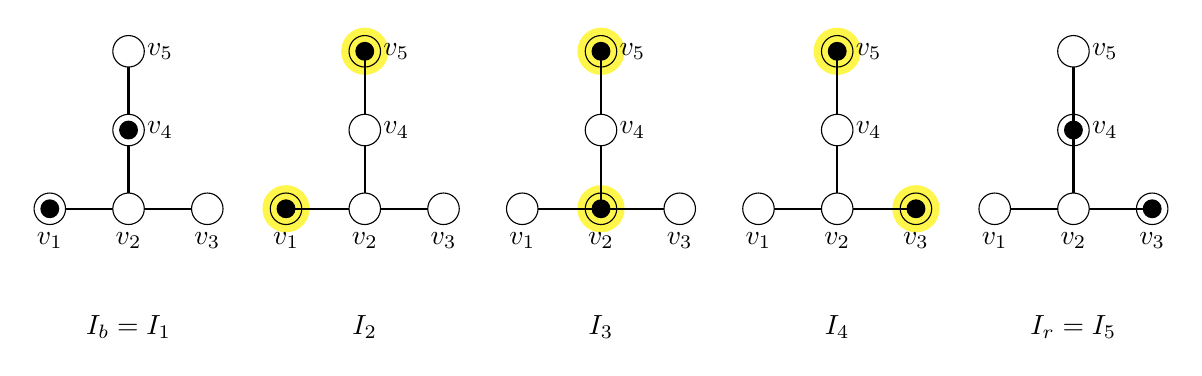
\begin{tikzpicture}[scale=1]
        \def\x{1}
        \def\xa{0}
        \def\ya{0}
        \def\xb{3}
        \def\xc{6}
        \def\xd{9}
        \def\xe{12}

        %graph G
        %edges
        \draw[thick] (\xa,\ya)--(\xa+1,\ya)--(\xa+1,\ya+1)--(\xa+1,\ya+2);
        \draw[thick] (\xa+1,\ya)--(\xa+2,\ya);
        %nodes
        \draw[fill=white] (\xa,\ya) circle (0.2cm);     %v1
        \draw[fill=white] (\xa+1,\ya+1) circle (0.2cm); %v2
        \draw[fill=white] (\xa+1,\ya+2) circle (0.2cm); %v3
        \draw[fill=white] (\xa+2,\ya) circle (0.2cm);   %v4
        \draw[fill=white] (\xa+1,\ya) circle (0.2cm);   %v5
        % Tokens
        \path[fill] (\xa+1,\ya+1) circle (\ver);
        \path[fill] (\xa,\ya) circle (\ver);
        %labels
        \node (1) at (\xa,\ya-0.4) {$v_1$};
        \node (2) at (\xa+1+0.4,\ya+1) {$v_4$};
        \node (3) at (\xa+1+0.4,\ya+2) {$v_5$};
        \node (5) at (\xa+2,\ya-0.4) {$v_3$};
        \node (4) at (\xa+1,\ya-0.4) {$v_2$};
        \node (1) at (\xa+1,\ya-1.5) {$I_b = I_1$};

        %G_1
        % Highlights
        \draw[fill=yellow, opacity=.7, draw=none] (\xb+1,\ya+2) circle (0.3cm);
        \draw[fill=yellow, opacity=.7, draw=none] (\xb,\ya)  circle (0.3cm);
        %edges
        \draw[thick] (\xb,\ya)--(\xb+1,\ya)--(\xb+1,\ya+1)--(\xb+1,\ya+2);
        \draw[thick] (\xb+1,\ya)--(\xb+2,\ya);
        %nodes
        \draw             (\xb,\ya) circle (0.2cm);    %v1
        \draw[fill=white] (\xb+1,\ya+1) circle (0.2cm);%v2
        \draw             (\xb+1,\ya+2) circle (0.2cm);%v3
        \draw[fill=white] (\xb+2,\ya) circle (0.2cm);  %v4
        \draw[fill=white] (\xb+1,\ya) circle (0.2cm);  %v5
        % Tokens
        \path[fill] (\xb+1,\ya+2) circle (\ver);
        \path[fill] (\xb,\ya) circle (\ver);
        %labels
        \node (1) at (\xb,\ya-0.4) {$v_1$};
        \node (2) at (\xb+1+0.4,\ya+1) {$v_4$};
        \node (3) at (\xb+1+0.4,\ya+2) {$v_5$};
        \node (5) at (\xb+2,\ya-0.4) {$v_3$};
        \node (4) at (\xb+1,\ya-0.4) {$v_2$};
        \node (1) at (\xb+1,\ya-1.5) {$I_2$};

        %G_2
        % Highlights
        \draw[fill=yellow, opacity=.7, draw=none] (\xc+1,\ya+2) circle (0.3cm);
        \draw[fill=yellow, opacity=.7, draw=none] (\xc+1,\ya)  circle (0.3cm);
        %edges
        \draw[thick] (\xc,\ya)--(\xc+1,\ya)--(\xc+1,\ya+1)--(\xc+1,\ya+2);
        \draw[thick] (\xc+1,\ya)--(\xc+2,\ya);
        %nodes
        \draw[fill=white] (\xc,\ya) circle (0.2cm);    %v1
        \draw[fill=white] (\xc+1,\ya+1) circle (0.2cm);%v2
        \draw             (\xc+1,\ya+2) circle (0.2cm);%v3
        \draw[fill=white] (\xc+2,\ya) circle (0.2cm);  %v4
        \draw             (\xc+1,\ya) circle (0.2cm);  %v5
        % Tokens
        \path[fill] (\xc+1,\ya+2) circle (\ver);
        \path[fill] (\xc+1,\ya)  circle (\ver);
        %labels
        \node (1) at (\xc,\ya-0.4) {$v_1$};
        \node (2) at (\xc+1+0.4,\ya+1) {$v_4$};
        \node (3) at (\xc+1+0.4,\ya+2) {$v_5$};
        \node (5) at (\xc+2,\ya-0.4) {$v_3$};
        \node (4) at (\xc+1,\ya-0.4) {$v_2$};
        \node (1) at (\xc+1,\ya-1.5) {$I_3$};

        %G_3
        % Highlights
        \draw[fill=yellow, opacity=.7, draw=none] (\xd+1,\ya+2) circle (0.3cm);
        \draw[fill=yellow, opacity=.7, draw=none] (\xd+2,\ya)  circle (0.3cm);
        %edges
        \draw[thick] (\xd,\ya)--(\xd+1,\ya)--(\xd+1,\ya+1)--(\xd+1,\ya+2);
        \draw[thick] (\xd+1,\ya)--(\xd+2,\ya);
        %nodes
        \draw[fill=white] (\xd,\ya) circle (0.2cm);    %v1
        \draw[fill=white] (\xd+1,\ya+1) circle (0.2cm);%v2
        \draw             (\xd+1,\ya+2) circle (0.2cm);%v3
        \draw             (\xd+2,\ya) circle (0.2cm);  %v4
        \draw[fill=white] (\xd+1,\ya) circle (0.2cm);  %v5
        % Tokens
        \path[fill] (\xd+1,\ya+2)  circle (\ver);
        \path[fill] (\xd+2,\ya) circle (\ver);
        %labels
        \node (1) at (\xd,\ya-0.4) {$v_1$};
        \node (2) at (\xd+1+0.4,\ya+1) {$v_4$};
        \node (3) at (\xd+1+0.4,\ya+2) {$v_5$};
        \node (5) at (\xd+2,\ya-0.4) {$v_3$};
        \node (4) at (\xd+1,\ya-0.4) {$v_2$};
        \node (1) at (\xd+1,\ya-1.5) {$I_4$};

        %G4
        %edges
        \draw[thick] (\xe,\ya)--(\xe+1,\ya)--(\xe+1,\ya+1)--(\xe+1,\ya+2);
        \draw[thick] (\xe+1,\ya)--(\xe+2,\ya);
        %nodes
        \draw[fill=white] (\xe,\ya) circle (0.2cm);    %v1
        \draw             (\xe+1,\ya+1) circle (0.2cm);%v2
        \draw[fill=white] (\xe+1,\ya+2) circle (0.2cm);%v3
        \draw             (\xe+2,\ya) circle (0.2cm);  %v4
        \draw[fill=white] (\xe+1,\ya) circle (0.2cm);  %v5
        % Tokens
        \path[fill] (\xe+1,\ya+1)  circle (\ver);
        \path[fill] (\xe+2,\ya) circle (\ver);
        %labels
        \node (1) at (\xe,\ya-0.4) {$v_1$};
        \node (2) at (\xe+1+0.4,\ya+1) {$v_4$};
        \node (3) at (\xe+1+0.4,\ya+2) {$v_5$};
        \node (5) at (\xe+2,\ya-0.4) {$v_3$};
        \node (4) at (\xe+1,\ya-0.4) {$v_2$};
        \node (1) at (\xe+1,\ya-1.5) {$I_r = I_5$};
      \end{tikzpicture}
    \end{scaletikzpicturetowidth}
  \caption{TS sequence $ \langle I_1, I_2,\dots,I_5 \rangle$ of independent sets which transforms $I_b = I_1$ into $I_r = I_5$ where the vertices in independent sets are depicted by small black circles (tokens).}
  \label{fig:sliding_token_example}
\end{figure}

\subsection{Known results for the SLIDING TOKEN problem.}
Analogous to the Independent Set problem being the key problem among thousands of $\NP$-complete problems to prove $\NP$-hardness,
the SLIDING TOKEN problem plays an important role since several $\PSPACE$-hardness results have been proved using reductions from it.

For the sliding token problem, some polynomial time algorithms have been investigated as follows: Linear time algorithms have been shown
for cographs (also known as P4-free graphs) \cite{kaminski_complexity_2012} and trees \cite{2014arXiv1406.6576D}. Polynomial time algorithms
are shown for bipartite permutation graphs \cite{fox-epstein_sliding_2015}, and claw-free graphs \cite{bonsma_reconfiguring_2014}.
On the other hand, $\PSPACE$-completeness is shown for graphs of bounded treewidth \cite{mouawad_reconfiguration_2014}, and planar
graphs \cite{hearn_pspace-completeness_2004}.

\subsection{$\PSPACE$-completeness.}

In this section we go over the $\PSPACE$-completeness result of the SLIDING TOKEN problem, proved by a reduction from NCL. As seen in
section \ref{sec:ncl_results}, there are slightly different versions of decision problems for NCL and all of them are $\PSPACE-$complete.
For our purpose, we just need the version for the configuration-to-configuration for planar NCL. Recall that an instance of the
C2C planar NCL problem is defined on a $3-$regular, planar, directed graph where each edge has a weight $\in \{1,2\}$ and each vertex is
either and $AND$ or an $OR$ vertex. The proof of theorem \ref{theorem:ncl_sliding_token} is organised in sections
\ref{subsubsection:reduction_structure} to \ref{subsubsection:and_or} which explains the reduction structure, gadets used and how they are
connected together.

\subsubsection{Reduction structure.}\label{subsubsection:reduction_structure}
To show that the SLIDING TOKEN problem is $\PSPACE$-complete we provide a reduction from configuration-to-configuration for AND/OR graphs
such that the NCL instance is solvable if and only if the corresponding SLIDING TOKEN is solvable. The sliding token instance is constructed by
piecing together gadgets which emulates the directed edges, the AND vertices and the OR vertices of the given NCL instance.
We construct the corresponding NCL $AND$ and $OR$ vertex gadgets out of sliding-token subgraphs illustrated in figures
\ref{fig:and_gadget_sliding_token} and \ref{fig:or_gadget_sliding_token} respectively.

\subsubsection{The OR gadget and the AND gadget.}\label{subsubsection:or_and}
The construction of Fig.\ref{fig:and_gadget_sliding_token} satisfies the same constraints as an NCL $AND$ vertex, with the upper
token corresponding to the blue edge and both lower tokens corresponding to the red edges. The upper token can slide in only when both lower
tokens are slid out thus maintaining the flow constraint of an NCL AND vertex.
Likewise, the construction of Fig.\ref{fig:or_gadget_sliding_token} satisfies the same constraints as an NCL $OR$ vertex with the upper
and two lower tokens corresponding the the $OR$ blue edges. The upper token in the $OR$ gadget can slide in when  either lower token is slid
out and the internal token can then slide to one side or the other to make room. Here it is the internal token that ensures the NCL flow
constraint is satisfied by sliding on a appropriate vertex among the three internal nodes to force one among the outer tokens are slid in.

%%%%%%%%%%%%%%%%%%%%%%%%%%%%%%%%%%%%%%%%%%%% BEGINING OF A FIGURE : AND and OR gadget of Sliding Token %%%%%%%%%%%%%%%%%%%%%%%%%%%%%%%%%%%%
\begin{figure} [H]
  \begin{subfigure}[b]{0.4\textwidth}
    \centering
    \begin{scaletikzpicturetowidth}{\textwidth}
      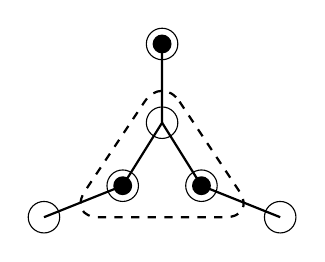
\begin{tikzpicture}
        \def\xa{0}
        \def\ya{0}
        %graph G
        \draw (\xa,\ya) circle (0.2cm);          %v1 no fill
        \draw (\xa,\ya+1) circle (0.2cm);        %v2 no fill
        \draw (\xa+0.5,\ya-0.8) circle (0.2cm);  %v4 no fill
        \draw (\xa-0.5,\ya-0.8) circle (0.2cm);  %v3 no fill
        \draw (\xa-1.5,\ya-1.2) circle (0.2cm);  %v5 no fill
        \draw (\xa+1.5,\ya-1.2) circle (0.2cm);  %v6 no fill
        \path[fill] (\xa,\ya+1) circle (\ver);       %v2
        \path[fill] (\xa+0.5,\ya-0.8) circle (\ver); %v4
        \path[fill] (\xa-0.5,\ya-0.8) circle (\ver); %v3
        %labels
        \draw[thick] (\xa,\ya+1)--(\xa,\ya)--(\xa-0.5,\ya-0.8)--(\xa-1.5,\ya-1.2);
        \draw[thick] (\xa,\ya)--(\xa+0.5,\ya-0.8)--(\xa+1.5,\ya-1.2);
        \path[draw, thick, dashed, rounded corners=4mm] (\xa,\ya+0.6)--(\xa+1.2,\ya-1.2)--(\xa-1.2,\ya-1.2)--cycle;
      \end{tikzpicture}
    \end{scaletikzpicturetowidth}
    \caption{$AND$ gadget}
    \label{fig:and_gadget_sliding_token}
  \end{subfigure}
  \hspace{3em} % vertical space
  \begin{subfigure}[b]{0.4\textwidth}
    \centering
    \begin{scaletikzpicturetowidth}{\textwidth}
      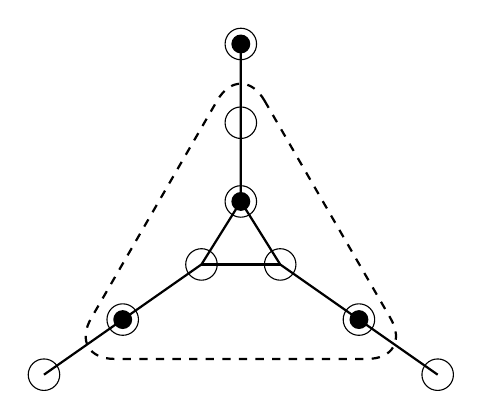
\begin{tikzpicture}
        \def\xb{5}
        \def\yb{0}
        %G_1
        \draw (\xb,\yb+2) circle (0.2cm);         %v9
        \draw (\xb,\yb) circle (0.2cm);           %v1
        \draw (\xb+0.5,\yb-0.8) circle (0.2cm);   %v4
        \draw (\xb-0.5,\yb-0.8) circle (0.2cm);   %v3
        \draw (\xb,\yb+1) circle (0.2cm);         %v2
        \draw (\xb-1.5,\yb-1.5) circle (0.2cm);   %v5
        \draw (\xb+1.5,\yb-1.5) circle (0.2cm);   %v6
        \draw (\xb-2.5,\yb-2.2) circle (0.2cm);     %v7
        \draw (\xb+2.5,\yb-2.2) circle (0.2cm);     %v8

        \path[fill] (\xb,\yb+2) circle (\ver);         %v0
        \path[fill] (\xb,\yb) circle (\ver);           %v1
        \path[fill] (\xb-1.5,\yb-1.5) circle (\ver);   %v5
        \path[fill] (\xb+1.5,\yb-1.5) circle (\ver);   %v6
        %labels
        \draw[thick] (\xb,\yb+2)--(\xb,\yb+1)--(\xb,\yb)--(\xb-0.5,\yb-0.8)--(\xb-1.5,\yb-1.5)--(\xb-2.5,\yb-2.2);
        \draw[thick] (\xb,\yb)--(\xb+0.5,\yb-0.8)--(\xb+1.5,\yb-1.5)--(\xb+2.5,\yb-2.2);
        \draw[thick] (\xb-0.5,\yb-0.8)--(\xb+0.5,\yb-0.8);
        \path[draw, thick, dashed, rounded corners=6mm] (\xb,\yb+1.8)--(\xb+2.2,\yb-2)--(\xb-2.2,\yb-2)--cycle;
      \end{tikzpicture}
    \end{scaletikzpicturetowidth}
    \caption{$OR$ gadget}
    \label{fig:or_gadget_sliding_token}
  \end{subfigure}
  \caption{Sliding Tokens vertex gadgets.}
  \label{fig:and_or_gadgets_sliding_token}
\end{figure}
%%%%%%%%%%%%%%%%%%%%%%%%%%%%%%%%%%%%%%%%%%%%%%%% ENDING OF A FIGURE %%%%%%%%%%%%%%%%%%%%%%%%%%%%%%%%%%%%%%%%%%%%%%%%

\subsubsection{AND/OR Graphs}\label{subsubsection:and_or}
We showed how to construct $AND$ and $OR$ vertices. We now show how to connect the vertices into an arbitrary planar constraint graph.
First, the edges that cross the dotted-line gadget borders are called “port” edges. A token on an outer port-edge vertex represents an
inward-directed NCL edge, and vice-versa. Second, observe that no port token may ever leave its port edge. Choosing a particular port
edge $E$, if we inductively assume that this condition holds for all other port edges, then there is never a legal move outside $E$ for
its token – another port token would have to leave its own edge first.
Given an $AND/OR$ graph $G$ and two legal configurations $C_1, C_2$ for $G$, we construct a corresponding sliding-token graph by joining together
$AND$ and $OR$ vertex gadgets at their shared port edges, placing the port tokens appropriately.


\begin{theorem}Sliding Token problem is $\PSPACE$-complete. \end{theorem}\label{theorem:ncl_sliding_token}
\begin{proof}
  First, we show that SLIDING TOKEN problem is in $\PSPACE$.
  The SLIDING TOKEN problem is in $\PSPACE$ since the state of the input graph can be described in a linear number of bits, specifying the
  position of each token and the list of possible moves from any state can be computed in polynomial time. Thus we can nondeterministically
  traverse the state space, at each step nondeterministically choosing a move to make , and maintaining the current state but not the previously
  visited states showing that SLIDING TOKEN is in $\NPSPACE$. By Savitch's celebrated theorem, we have that $\NPSPACE = \PSPACE$
  \cite{savitch_relationships_1970}, implying that SLIDING TOKEN is in $\PSPACE$.

  The SLIDING TOKEN problem is $\PSPACE$-hard by a reduction from planar Nondeterministic Constraint Logic using the reduction structure
  provided above. The NCL instance is solvable if and only if the corresponding SLIDING TOKEN is solvable.
\end{proof}

\begin{example}{C2E to SLIDING TOKEN problem reduction. \\}
\textbf{Input instance : C2E for restricted NCL.} \hfill

\begin{figure}[H]
  \centering
  \begin{subfigure}[b]{0.4\textwidth}
    \begin{scaletikzpicturetowidth}{\textwidth}
      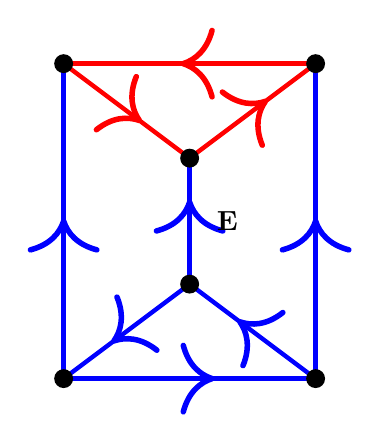
\begin{tikzpicture}[scale=0.8]
        \def\ver{0.15} %size of a vertex
        % v1
        \def\xa{0}
        \def\ya{0}
        % arrows
        \draw[middlearrow={<}, red] (\xa-2,\ya+1.5)-- (\xa+2,\ya+1.5);        % v2 - v3
        \draw[middlearrow={<}, red] (\xa+2,\ya+1.5) -- (\xa,\ya);             % v3 - v1
        \draw[middlearrow={<}, red] (\xa,\ya) -- (\xa-2,\ya+1.5);             % v1 - v2
        \draw[middlearrow={<}, blue] (\xa-2,\ya+1.5) -- (\xa-2,\ya-3.5);      % v2 - v4
        \draw[middlearrow={<}, blue] (\xa,\ya) -- (\xa,\ya-2);                % v1 - v6
        \draw[middlearrow={<}, blue] (\xa+2,\ya+1.5) -- (\xa+2,\ya-3.5);      % v3 - v5
        \draw[middlearrow={>}, blue] (\xa-2,\ya-3.5) -- (\xa+2,\ya-3.5);      % v4 - v5
        \draw[middlearrow={<}, blue] (\xa-2,\ya-3.5) -- (\xa,\ya-2);          % v4 - v6
        \draw[middlearrow={<}, blue] (\xa,\ya-2) -- (\xa+2,\ya-3.5);          % v6 - v5
        % edges
        \draw[ultra thick, -, red] (\xa-2,\ya+1.5) -- (\xa+2,\ya+1.5);       % v2 - v3
        \draw[ultra thick, -, red] (\xa+2,\ya+1.5) -- (\xa,\ya);             % v3 - v1
        \draw[ultra thick, -, red] (\xa,\ya) -- (\xa-2,\ya+1.5);             % v1 - v2
        \draw[ultra thick, -, blue] (\xa-2,\ya+1.5) -- (\xa-2,\ya-3.5);      % v2 - v4
        \draw[ultra thick, -, blue] (\xa,\ya) -- (\xa,\ya-2);                % v1 - v6
        \draw[ultra thick, -, blue] (\xa+2,\ya+1.5) -- (\xa+2,\ya-3.5);      % v3 - v5
        \draw[ultra thick, -, blue] (\xa-2,\ya-3.5) -- (\xa+2,\ya-3.5);      % v4 - v5
        \draw[ultra thick, -, blue] (\xa-2,\ya-3.5) -- (\xa,\ya-2);          % v4 - v6
        \draw[ultra thick, -, blue] (\xa,\ya-2) -- (\xa+2,\ya-3.5);          % v6 - v5

        \node (a) at (\xa+0.6,\ya-1) {\textbf{E}};

        %graph G : Nodes fill
        \path[fill] (\xa,\ya) circle (\ver);           %v1
        \path[fill] (\xa-2,\ya+1.5) circle (\ver);     %v2
        \path[fill] (\xa+2,\ya+1.5) circle (\ver);     %v3
        \path[fill] (\xa-2,\ya-3.5) circle (\ver);     %v4
        \path[fill] (\xa+2,\ya-3.5) circle (\ver);     %v5
        \path[fill] (\xa,\ya-2) circle (\ver);         %v6
      \end{tikzpicture}
    \end{scaletikzpicturetowidth}
    \caption{$C_0$}
    \label{fig:input_instance}
  \end{subfigure}
  \begin{subfigure}[b]{0.4\textwidth}
    \begin{scaletikzpicturetowidth}{\textwidth}
      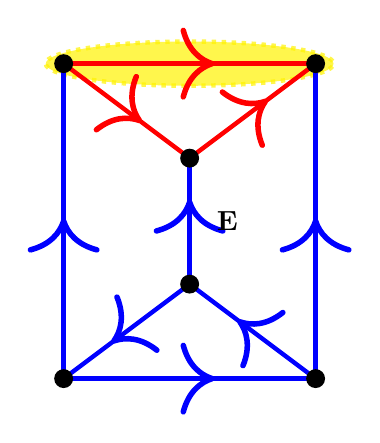
\begin{tikzpicture}[scale=0.8]
        \def\ver{0.15} %size of a vertex
        % v1
        \def\xa{0}
        \def\ya{0}
        % Highlight change
        \draw[fill=yellow, opacity=.7, ultra thick, dotted, rotate around={90:(\xa,\ya+1.5)},yellow] (\xa,\ya+1.5) ellipse (10pt and 65pt);
        % f_1 arrows
        \draw[middlearrow={>}, red] (\xa-2,\ya+1.5)-- (\xa+2,\ya+1.5);        % v2 - v3
        \draw[middlearrow={<}, red] (\xa+2,\ya+1.5) -- (\xa,\ya);             % v3 - v1
        \draw[middlearrow={<}, red] (\xa,\ya) -- (\xa-2,\ya+1.5);             % v1 - v2
        \draw[middlearrow={<}, blue] (\xa-2,\ya+1.5) -- (\xa-2,\ya-3.5);      % v2 - v4
        \draw[middlearrow={<}, blue] (\xa,\ya) -- (\xa,\ya-2);                % v1 - v6
        \draw[middlearrow={<}, blue] (\xa+2,\ya+1.5) -- (\xa+2,\ya-3.5);      % v3 - v5
        \draw[middlearrow={>}, blue] (\xa-2,\ya-3.5) -- (\xa+2,\ya-3.5);      % v4 - v5
        \draw[middlearrow={<}, blue] (\xa-2,\ya-3.5) -- (\xa,\ya-2);          % v4 - v6
        \draw[middlearrow={<}, blue] (\xa,\ya-2) -- (\xa+2,\ya-3.5);          % v6 - v5

        \draw[ultra thick, -, red] (\xa-2,\ya+1.5) -- (\xa+2,\ya+1.5);       % v2 - v3
        \draw[ultra thick, -, red] (\xa+2,\ya+1.5) -- (\xa,\ya);             % v3 - v1
        \draw[ultra thick, -, red] (\xa,\ya) -- (\xa-2,\ya+1.5);             % v1 - v2
        \draw[ultra thick, -, blue] (\xa-2,\ya+1.5) -- (\xa-2,\ya-3.5);      % v2 - v4
        \draw[ultra thick, -, blue] (\xa,\ya) -- (\xa,\ya-2);                % v1 - v6
        \draw[ultra thick, -, blue] (\xa+2,\ya+1.5) -- (\xa+2,\ya-3.5);      % v3 - v5
        \draw[ultra thick, -, blue] (\xa-2,\ya-3.5) -- (\xa+2,\ya-3.5);      % v4 - v5
        \draw[ultra thick, -, blue] (\xa-2,\ya-3.5) -- (\xa,\ya-2);          % v4 - v6
        \draw[ultra thick, -, blue] (\xa,\ya-2) -- (\xa+2,\ya-3.5);          % v6 - v5

        \node (a) at (\xa+0.6,\ya-1) {\textbf{E}};

        %graph G : Nodes fill
        \path[fill] (\xa,\ya) circle (\ver);           %v1
        \path[fill] (\xa-2,\ya+1.5) circle (\ver);   %v2
        \path[fill] (\xa+2,\ya+1.5) circle (\ver);   %v3
        \path[fill] (\xa-2,\ya-3.5) circle (\ver);   %v4
        \path[fill] (\xa+2,\ya-3.5) circle (\ver);   %v5
        \path[fill] (\xa,\ya-2) circle (\ver);         %v6
      \end{tikzpicture}
    \end{scaletikzpicturetowidth}
    \caption{$C_1$}
    \label{fig:input_instance_1}
  \end{subfigure}
  \begin{subfigure}[b]{0.4\textwidth}
    \begin{scaletikzpicturetowidth}{\textwidth}
      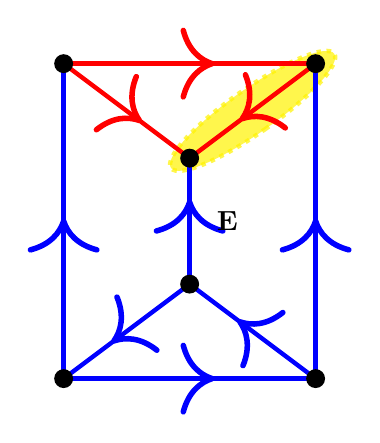
\begin{tikzpicture}[scale=0.8]
        \def\ver{0.15} %size of a vertex
        % v1
        \def\xa{0}
        \def\ya{0}
        % Highlight change
        \draw[fill=yellow, opacity=.7, ultra thick, dotted, rotate around={305:(\xa+1,\ya+0.75)},yellow] (\xa+1,\ya+0.75) ellipse (10pt and 45pt);
        % f_1 arrows
        \draw[middlearrow={>}, red] (\xa-2,\ya+1.5)-- (\xa+2,\ya+1.5);        % v2 - v3
        \draw[middlearrow={>}, red] (\xa+2,\ya+1.5) -- (\xa,\ya);             % v3 - v1
        \draw[middlearrow={<}, red] (\xa,\ya) -- (\xa-2,\ya+1.5);             % v1 - v2
        \draw[middlearrow={<}, blue] (\xa-2,\ya+1.5) -- (\xa-2,\ya-3.5);      % v2 - v4
        \draw[middlearrow={<}, blue] (\xa,\ya) -- (\xa,\ya-2);                % v1 - v6
        \draw[middlearrow={<}, blue] (\xa+2,\ya+1.5) -- (\xa+2,\ya-3.5);      % v3 - v5
        \draw[middlearrow={>}, blue] (\xa-2,\ya-3.5) -- (\xa+2,\ya-3.5);      % v4 - v5
        \draw[middlearrow={<}, blue] (\xa-2,\ya-3.5) -- (\xa,\ya-2);          % v4 - v6
        \draw[middlearrow={<}, blue] (\xa,\ya-2) -- (\xa+2,\ya-3.5);          % v6 - v5

        \draw[ultra thick, -, red] (\xa-2,\ya+1.5) -- (\xa+2,\ya+1.5);       % v2 - v3
        \draw[ultra thick, -, red] (\xa+2,\ya+1.5) -- (\xa,\ya);             % v3 - v1
        \draw[ultra thick, -, red] (\xa,\ya) -- (\xa-2,\ya+1.5);             % v1 - v2
        \draw[ultra thick, -, blue] (\xa-2,\ya+1.5) -- (\xa-2,\ya-3.5);      % v2 - v4
        \draw[ultra thick, -, blue] (\xa,\ya) -- (\xa,\ya-2);                % v1 - v6
        \draw[ultra thick, -, blue] (\xa+2,\ya+1.5) -- (\xa+2,\ya-3.5);      % v3 - v5
        \draw[ultra thick, -, blue] (\xa-2,\ya-3.5) -- (\xa+2,\ya-3.5);      % v4 - v5
        \draw[ultra thick, -, blue] (\xa-2,\ya-3.5) -- (\xa,\ya-2);          % v4 - v6
        \draw[ultra thick, -, blue] (\xa,\ya-2) -- (\xa+2,\ya-3.5);          % v6 - v5

        \node (a) at (\xa+0.6,\ya-1) {\textbf{E}};

        %graph G : Nodes fill
        \path[fill] (\xa,\ya) circle (\ver);           %v1
        \path[fill] (\xa-2,\ya+1.5) circle (\ver);   %v2
        \path[fill] (\xa+2,\ya+1.5) circle (\ver);   %v3
        \path[fill] (\xa-2,\ya-3.5) circle (\ver);   %v4
        \path[fill] (\xa+2,\ya-3.5) circle (\ver);   %v5
        \path[fill] (\xa,\ya-2) circle (\ver);         %v6
      \end{tikzpicture}
    \end{scaletikzpicturetowidth}
    \caption{$C_2$}
    \label{fig:input_instance_2}
  \end{subfigure}
  \begin{subfigure}[b]{0.4\textwidth}
    \begin{scaletikzpicturetowidth}{\textwidth}
      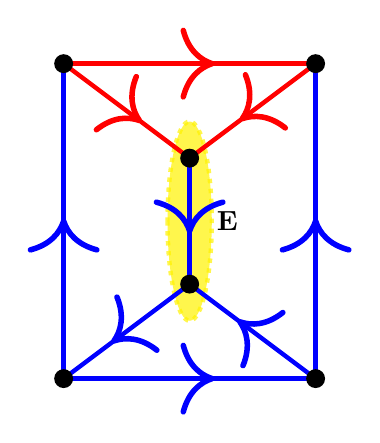
\begin{tikzpicture}[scale=0.8]
        \def\ver{0.15} %size of a vertex
        % v1
        \def\xa{0}
        \def\ya{0}
        % Highlight change
        \draw[fill=yellow, opacity=.7, ultra thick, dotted, rotate around={180:(\xa,\ya-1)},yellow] (\xa,\ya-1) ellipse (10pt and 45pt);
        % f_1 arrows
        \draw[middlearrow={>}, red] (\xa-2,\ya+1.5)-- (\xa+2,\ya+1.5);        % v2 - v3
        \draw[middlearrow={>}, red] (\xa+2,\ya+1.5) -- (\xa,\ya);             % v3 - v1
        \draw[middlearrow={<}, red] (\xa,\ya) -- (\xa-2,\ya+1.5);             % v1 - v2
        \draw[middlearrow={<}, blue] (\xa-2,\ya+1.5) -- (\xa-2,\ya-3.5);      % v2 - v4
        \draw[middlearrow={>}, blue] (\xa,\ya) -- (\xa,\ya-2);                % v1 - v6
        \draw[middlearrow={<}, blue] (\xa+2,\ya+1.5) -- (\xa+2,\ya-3.5);      % v3 - v5
        \draw[middlearrow={>}, blue] (\xa-2,\ya-3.5) -- (\xa+2,\ya-3.5);      % v4 - v5
        \draw[middlearrow={<}, blue] (\xa-2,\ya-3.5) -- (\xa,\ya-2);          % v4 - v6
        \draw[middlearrow={<}, blue] (\xa,\ya-2) -- (\xa+2,\ya-3.5);          % v6 - v5

        \draw[ultra thick, -, red] (\xa-2,\ya+1.5) -- (\xa+2,\ya+1.5);       % v2 - v3
        \draw[ultra thick, -, red] (\xa+2,\ya+1.5) -- (\xa,\ya);             % v3 - v1
        \draw[ultra thick, -, red] (\xa,\ya) -- (\xa-2,\ya+1.5);             % v1 - v2
        \draw[ultra thick, -, blue] (\xa-2,\ya+1.5) -- (\xa-2,\ya-3.5);      % v2 - v4
        \draw[ultra thick, -, blue] (\xa,\ya) -- (\xa,\ya-2);                % v1 - v6
        \draw[ultra thick, -, blue] (\xa+2,\ya+1.5) -- (\xa+2,\ya-3.5);      % v3 - v5
        \draw[ultra thick, -, blue] (\xa-2,\ya-3.5) -- (\xa+2,\ya-3.5);      % v4 - v5
        \draw[ultra thick, -, blue] (\xa-2,\ya-3.5) -- (\xa,\ya-2);          % v4 - v6
        \draw[ultra thick, -, blue] (\xa,\ya-2) -- (\xa+2,\ya-3.5);          % v6 - v5

        \node (a) at (\xa+0.6,\ya-1) {\textbf{E}};            % Label reject

        %graph G : Nodes fill
        \path[fill] (\xa,\ya) circle (\ver);           %v1
        \path[fill] (\xa-2,\ya+1.5) circle (\ver);   %v2
        \path[fill] (\xa+2,\ya+1.5) circle (\ver);   %v3
        \path[fill] (\xa-2,\ya-3.5) circle (\ver);   %v4
        \path[fill] (\xa+2,\ya-3.5) circle (\ver);   %v5
        \path[fill] (\xa,\ya-2) circle (\ver);         %v6
      \end{tikzpicture}
    \end{scaletikzpicturetowidth}
    \caption{$C_3$}
    \label{fig:input_instance_3}
  \end{subfigure}
  \caption{Reconfiguration sequence which transforms $C_0$ which is the initial configuration into $C_3 = $ which is the target configuration.}
  \label{fig:input_instance_config_to_edge}
\end{figure}

%%%%%%%%%%%%%%%%%%%%%%%%%%%%%%%%%%%%%%%%%%% Output instance %%%%%%%%%%%%%%%%%%%%%%%%%%%%%%%%
%------------------------------------------- out 1 & 2 ---------------------------------------------
\textbf{Output instance : SLIDING TOKEN instance.} \hfill

\begin{figure}[H]
  \raggedright
  \begin{subfigure}[b]{0.6\textwidth}
    \begin{scaletikzpicturetowidth}{\textwidth}
      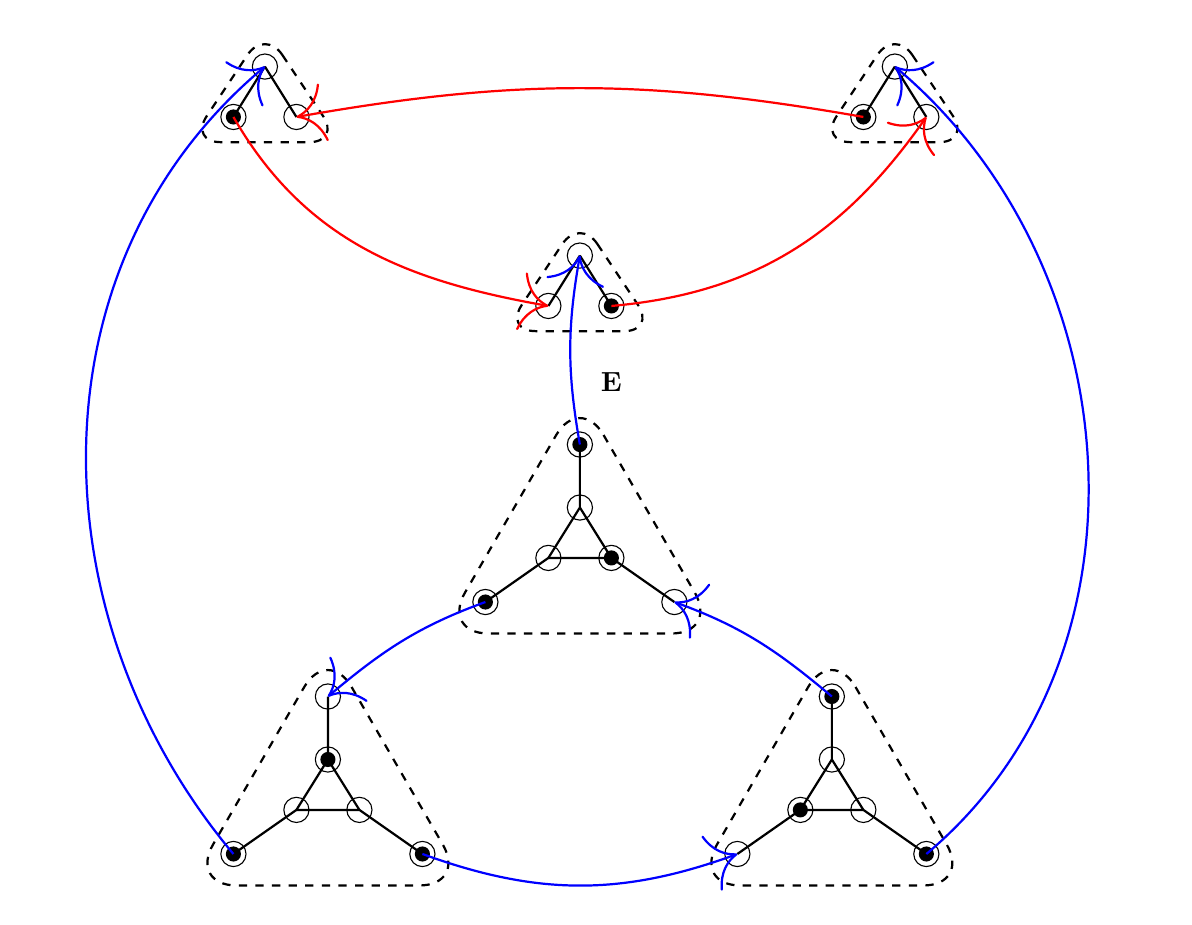
\begin{tikzpicture}[scale=0.8]
        %%%%%%%%%%%% AND 1 %%%%%%%%%%%%
        \def\ver{0.12} %size of a vertex
        \def\xa{-1}
        \def\ya{0}
        % Highlight change
        %graph G
        \draw (\xa,\ya) circle (0.2cm);          %v1 no fill
        \draw (\xa+0.5,\ya-0.8) circle (0.2cm);  %v4 no fill
        \draw (\xa-0.5,\ya-0.8) circle (0.2cm);  %v3 no fill
        % Tokens
        \path[fill] (\xa-0.5,\ya-0.8) circle (\ver);   %v3
        %labels
        \draw[thick] (\xa,\ya)--(\xa-0.5,\ya-0.8);
        \draw[thick] (\xa,\ya)--(\xa+0.5,\ya-0.8);
        \path[draw, thick, dashed, rounded corners=4mm] (\xa,\ya+0.6)--(\xa+1.2,\ya-1.2)--(\xa-1.2,\ya-1.2)--cycle;
        %%%%%%%%%%%% AND 2 %%%%%%%%%%%%
        \def\ver{0.12} %size of a vertex
        \def\xb{4}
        \def\yb{-3}
        %graph G
        \draw (\xb,\yb) circle (0.2cm);          %v1 no fill
        \draw (\xb+0.5,\yb-0.8) circle (0.2cm);  %v4 no fill
        \draw (\xb-0.5,\yb-0.8) circle (0.2cm);  %v3 no fill
        % Tokens
        \path[fill] (\xb+0.5,\yb-0.8) circle (\ver);   %v3
        %labels
        \draw[thick] (\xb,\yb)--(\xb-0.5,\yb-0.8);
        \draw[thick] (\xb,\yb)--(\xb+0.5,\yb-0.8);
        \path[draw, thick, dashed, rounded corners=4mm] (\xb,\yb+0.6)--(\xb+1.2,\yb-1.2)--(\xb-1.2,\yb-1.2)--cycle;
        %%%%%%%%%%%% AND 3 %%%%%%%%%%%%
        \def\ver{0.12} %size of a vertex
        \def\xc{9}
        \def\yc{0}
        %graph G
        \draw (\xc,\yc) circle (0.2cm);          %v1 no fill
        \draw (\xc+0.5,\yc-0.8) circle (0.2cm);  %v4 no fill
        \draw (\xc-0.5,\yc-0.8) circle (0.2cm);  %v3 no fill
        % Tokens
        \path[fill] (\xc-0.5,\yc-0.8) circle (\ver);   %v3
        %labels
        \draw[thick] (\xc,\yc)--(\xc-0.5,\yc-0.8);
        \draw[thick] (\xc,\yc)--(\xc+0.5,\yc-0.8);
        \path[draw, thick, dashed, rounded corners=4mm] (\xc,\yc+0.6)--(\xc+1.2,\yc-1.2)--(\xc-1.2,\yc-1.2)--cycle;
        %%%%%%%%%%%% OR 1 %%%%%%%%%%%%
        \def\ver{0.12} %size of a vertex
        \def\xd{0}
        \def\yd{-11}
        %G_1
        \draw (\xd,\yd) circle (0.2cm);           %v1
        \draw (\xd+0.5,\yd-0.8) circle (0.2cm);   %v4
        \draw (\xd-0.5,\yd-0.8) circle (0.2cm);   %v3
        \draw (\xd,\yd+1) circle (0.2cm);         %v2
        \draw (\xd-1.5,\yd-1.5) circle (0.2cm);   %v5
        \draw (\xd+1.5,\yd-1.5) circle (0.2cm);   %v6
        \path[fill] (\xd,\yd) circle (\ver);           %v1
        \path[fill] (\xd-1.5,\yd-1.5) circle (\ver);   %v5
        \path[fill] (\xd+1.5,\yd-1.5) circle (\ver);   %v6
        %labels
        \draw[thick] (\xd,\yd+1)--(\xd, \yd)--(\xd-0.5,\yd-0.8)--(\xd-1.5,\yd-1.5);
        \draw[thick] (\xd-0.5,\yd-0.8)--(\xd+0.5,\yd-0.8)--(\xd+1.5,\yd-1.5);
        \draw[thick] (\xd,\yd)-- (\xd+0.5,\yd-0.8);

        \path[draw, thick, dashed, rounded corners=6mm] (\xd,\yd+1.8)--(\xd+2.2,\yd-2)--(\xd-2.2,\yd-2)--cycle;
        %%%%%%%%%%%% OR 2 %%%%%%%%%%%%
        \def\ver{0.12} %size of a vertex
        \def\xe{4}
        \def\ye{-7}
        %G_1
        \draw (\xe,\ye) circle (0.2cm);           %v1
        \draw (\xe+0.5,\ye-0.8) circle (0.2cm);   %v4
        \draw (\xe-0.5,\ye-0.8) circle (0.2cm);   %v3
        \draw (\xe,\ye+1) circle (0.2cm);         %v2
        \draw (\xe-1.5,\ye-1.5) circle (0.2cm);   %v5
        \draw (\xe+1.5,\ye-1.5) circle (0.2cm);   %v6

        \path[fill] (\xe,\ye+1) circle (\ver);         %v2
        \path[fill] (\xe+0.5,\ye-0.8) circle (\ver);   %v4
        \path[fill] (\xe-1.5,\ye-1.5) circle (\ver);   %v5
        %labels
        \draw[thick] (\xe,\ye+1)--(\xe, \ye)--(\xe-0.5,\ye-0.8)--(\xe-1.5,\ye-1.5);
        \draw[thick] (\xe-0.5,\ye-0.8)--(\xe+0.5,\ye-0.8)--(\xe+1.5,\ye-1.5);
        \draw[thick] (\xe,\ye)-- (\xe+0.5,\ye-0.8);
        \path[draw, thick, dashed, rounded corners=6mm] (\xe,\ye+1.8)--(\xe+2.2,\ye-2)--(\xe-2.2,\ye-2)--cycle;
        %%%%%%%%%%%% OR 3 %%%%%%%%%%%%
        \def\ver{0.12} %size of a vertex
        \def\xf{8}
        \def\yf{-11}
        %G_1
        \draw (\xf,\yf) circle (0.2cm);           %v1
        \draw (\xf+0.5,\yf-0.8) circle (0.2cm);   %v4
        \draw (\xf-0.5,\yf-0.8) circle (0.2cm);   %v3
        \draw (\xf,\yf+1) circle (0.2cm);         %v2
        \draw (\xf-1.5,\yf-1.5) circle (0.2cm);   %v5
        \draw (\xf+1.5,\yf-1.5) circle (0.2cm);   %v6

        \path[fill] (\xf,\yf+1) circle (\ver);         %v2
        \path[fill] (\xf-0.5,\yf-0.8) circle (\ver);   %v3
        \path[fill] (\xf+1.5,\yf-1.5) circle (\ver);   %v6
        %labels
        \draw[thick] (\xf,\yf+1)--(\xf, \yf)--(\xf-0.5,\yf-0.8)--(\xf-1.5,\yf-1.5);
        \draw[thick] (\xf-0.5,\yf-0.8)--(\xf+0.5,\yf-0.8)--(\xf+1.5,\yf-1.5);
        \draw[thick] (\xf,\yf)-- (\xf+0.5,\yf-0.8);
        \path[draw, thick, dashed, rounded corners=6mm] (\xf,\yf+1.8)--(\xf+2.2,\yf-2)--(\xf-2.2,\yf-2)--cycle;
        %%%%%%%%%%% EDGES %%%%%%%%%
        \node (a) at (4.5,-5) {\textbf{E}};            % Label reject
        \draw [-, red, thick, arrows={->[scale=3,red]}] (\xc-0.5,\yc-0.8) to [out=170,in=10] (\xa+0.5,\ya-0.8);            % AND 3  -- AND 1
        \draw [-, red, thick, arrows={->[scale=3,red]}] (\xa-0.5,\ya-0.8)  to [out=300,in=170] (\xb-0.5,\yb-0.8);          % AND 1  -- AND 2
        \draw [-, red, thick, arrows={->[scale=3,red]}] (\xb+0.5,\yb-0.8) to [out=5,in=235] (\xc+0.5,\yc-0.8);             % AND 2  -- AND 3
        \draw [-, blue, thick, arrows={->[scale=3,blue]}] (\xd-1.5,\yd-1.5) to [out=130,in=220] (\xa,\ya);                 % OR 1  -- AND 1
        \draw [-, blue, thick, arrows={->[scale=3,blue]}] (\xd+1.5,\yd-1.5) to [out=340,in=200] (\xf-1.5,\yf-1.5);         % OR 1  -- OR 3
        \draw [-, blue, thick, arrows={->[scale=3,blue]}] (\xf,\yf+1)  to [out=140,in=340] (\xe+1.5,\ye-1.5);              % OR 3  -- OR 2
        \draw [-, blue, thick, arrows={->[scale=3,blue]}] (\xe-1.5,\ye-1.5) to [out=200,in=40] (\xd,\yd+1);                % OR 2  -- OR 1
        \draw [-, blue, thick, arrows={->[scale=3,blue]}] (\xf+1.5,\yf-1.5) to [out=40,in=320] (\xc,\yc);                  % OR 3  -- AND 3
        \draw [-, blue, thick, arrows={->[scale=3,blue]}] (\xe,\ye+1) to [out=100,in=260] (\xb,\yb);                       % OR 2  -- AND 2
      \end{tikzpicture}
    \end{scaletikzpicturetowidth}
  \caption{$S_0$.}
  \label{fig:output_instance_final}
  \end{subfigure}
  \vspace{3em}
  \begin{subfigure}[b]{0.6\textwidth}
    \begin{scaletikzpicturetowidth}{\textwidth}
      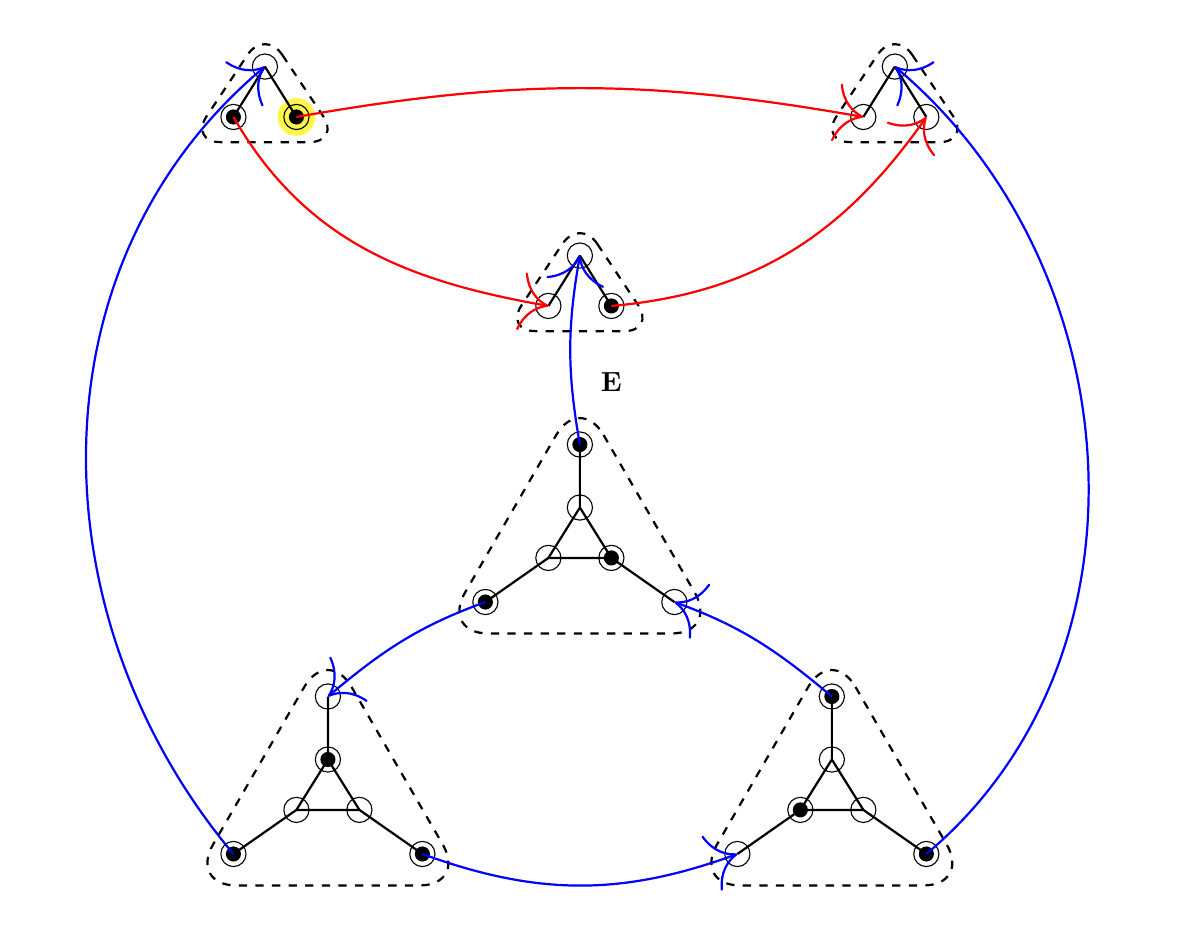
\begin{tikzpicture}[scale=0.8]
        %%%%%%%%%%%% AND 1 %%%%%%%%%%%%
        \def\ver{0.12} %size of a vertex
        \def\xa{-1}
        \def\ya{0}
        % Highlight change
        \draw[fill=yellow, opacity=.7, draw=none] (\xa+0.5,\ya-0.8) circle (0.3cm);
        %\draw[fill=yellow, opacity=.7, draw=none] (\xa-0.5,\ya-0.8) circle (0.3cm);
        %graph G
        \draw (\xa,\ya) circle (0.2cm);          %v1 no fill
        \draw (\xa+0.5,\ya-0.8) circle (0.2cm);  %v4 no fill
        \draw (\xa-0.5,\ya-0.8) circle (0.2cm);  %v3 no fill
        % Tokens
        \path[fill] (\xa-0.5,\ya-0.8) circle (\ver);   %v3
        \path[fill] (\xa+0.5,\ya-0.8) circle (\ver);   %v4
        %labels
        \draw[thick] (\xa,\ya)--(\xa-0.5,\ya-0.8);
        \draw[thick] (\xa,\ya)--(\xa+0.5,\ya-0.8);
        \path[draw, thick, dashed, rounded corners=4mm] (\xa,\ya+0.6)--(\xa+1.2,\ya-1.2)--(\xa-1.2,\ya-1.2)--cycle;
        %%%%%%%%%%%% AND 2 %%%%%%%%%%%%
        \def\ver{0.12} %size of a vertex
        \def\xb{4}
        \def\yb{-3}
        %graph G
        \draw (\xb,\yb) circle (0.2cm);          %v1 no fill
        \draw (\xb+0.5,\yb-0.8) circle (0.2cm);  %v4 no fill
        \draw (\xb-0.5,\yb-0.8) circle (0.2cm);  %v3 no fill
        % Tokens
        \path[fill] (\xb+0.5,\yb-0.8) circle (\ver);   %v3
        %labels
        \draw[thick] (\xb,\yb)--(\xb-0.5,\yb-0.8);
        \draw[thick] (\xb,\yb)--(\xb+0.5,\yb-0.8);
        \path[draw, thick, dashed, rounded corners=4mm] (\xb,\yb+0.6)--(\xb+1.2,\yb-1.2)--(\xb-1.2,\yb-1.2)--cycle;
        %%%%%%%%%%%% AND 3 %%%%%%%%%%%%
        \def\ver{0.12} %size of a vertex
        \def\xc{9}
        \def\yc{0}
        %graph G
        \draw (\xc,\yc) circle (0.2cm);          %v1 no fill
        \draw (\xc+0.5,\yc-0.8) circle (0.2cm);  %v4 no fill
        \draw (\xc-0.5,\yc-0.8) circle (0.2cm);  %v3 no fill
        %labels
        \draw[thick] (\xc,\yc)--(\xc-0.5,\yc-0.8);
        \draw[thick] (\xc,\yc)--(\xc+0.5,\yc-0.8);
        \path[draw, thick, dashed, rounded corners=4mm] (\xc,\yc+0.6)--(\xc+1.2,\yc-1.2)--(\xc-1.2,\yc-1.2)--cycle;
        %%%%%%%%%%%% OR 1 %%%%%%%%%%%%
        \def\ver{0.12} %size of a vertex
        \def\xd{0}
        \def\yd{-11}
        %G_1
        \draw (\xd,\yd) circle (0.2cm);           %v1
        \draw (\xd+0.5,\yd-0.8) circle (0.2cm);   %v4
        \draw (\xd-0.5,\yd-0.8) circle (0.2cm);   %v3
        \draw (\xd,\yd+1) circle (0.2cm);         %v2
        \draw (\xd-1.5,\yd-1.5) circle (0.2cm);   %v5
        \draw (\xd+1.5,\yd-1.5) circle (0.2cm);   %v6

        \path[fill] (\xd,\yd) circle (\ver);           %v1
        \path[fill] (\xd-1.5,\yd-1.5) circle (\ver);   %v5
        \path[fill] (\xd+1.5,\yd-1.5) circle (\ver);   %v6
        %labels
        \draw[thick] (\xd,\yd+1)--(\xd, \yd)--(\xd-0.5,\yd-0.8)--(\xd-1.5,\yd-1.5);
        \draw[thick] (\xd-0.5,\yd-0.8)--(\xd+0.5,\yd-0.8)--(\xd+1.5,\yd-1.5);
        \draw[thick] (\xd,\yd)-- (\xd+0.5,\yd-0.8);
        \path[draw, thick, dashed, rounded corners=6mm] (\xd,\yd+1.8)--(\xd+2.2,\yd-2)--(\xd-2.2,\yd-2)--cycle;
        %%%%%%%%%%%% OR 2 %%%%%%%%%%%%
        \def\ver{0.12} %size of a vertex
        \def\xe{4}
        \def\ye{-7}
        %G_1
        \draw (\xe,\ye) circle (0.2cm);           %v1
        \draw (\xe+0.5,\ye-0.8) circle (0.2cm);   %v4
        \draw (\xe-0.5,\ye-0.8) circle (0.2cm);   %v3
        \draw (\xe,\ye+1) circle (0.2cm);         %v2
        \draw (\xe-1.5,\ye-1.5) circle (0.2cm);   %v5
        \draw (\xe+1.5,\ye-1.5) circle (0.2cm);   %v6
        \path[fill] (\xe,\ye+1) circle (\ver);         %v2
        \path[fill] (\xe+0.5,\ye-0.8) circle (\ver);   %v4
        \path[fill] (\xe-1.5,\ye-1.5) circle (\ver);   %v5
        %labels
        \draw[thick] (\xe,\ye+1)--(\xe, \ye)--(\xe-0.5,\ye-0.8)--(\xe-1.5,\ye-1.5);
        \draw[thick] (\xe-0.5,\ye-0.8)--(\xe+0.5,\ye-0.8)--(\xe+1.5,\ye-1.5);
        \draw[thick] (\xe,\ye)-- (\xe+0.5,\ye-0.8);
        \path[draw, thick, dashed, rounded corners=6mm] (\xe,\ye+1.8)--(\xe+2.2,\ye-2)--(\xe-2.2,\ye-2)--cycle;
        %%%%%%%%%%%% OR 3 %%%%%%%%%%%%
        \def\ver{0.12} %size of a vertex
        \def\xf{8}
        \def\yf{-11}
        %G_1
        \draw (\xf,\yf) circle (0.2cm);           %v1
        \draw (\xf+0.5,\yf-0.8) circle (0.2cm);   %v4
        \draw (\xf-0.5,\yf-0.8) circle (0.2cm);   %v3
        \draw (\xf,\yf+1) circle (0.2cm);         %v2
        \draw (\xf-1.5,\yf-1.5) circle (0.2cm);   %v5
        \draw (\xf+1.5,\yf-1.5) circle (0.2cm);   %v6
        %tokens
        \path[fill] (\xf,\yf+1) circle (\ver);         %v2
        \path[fill] (\xf-0.5,\yf-0.8) circle (\ver);   %v3
        \path[fill] (\xf+1.5,\yf-1.5) circle (\ver);   %v6
        %labels
        \draw[thick] (\xf,\yf+1)--(\xf, \yf)--(\xf-0.5,\yf-0.8)--(\xf-1.5,\yf-1.5);
        \draw[thick] (\xf-0.5,\yf-0.8)--(\xf+0.5,\yf-0.8)--(\xf+1.5,\yf-1.5);
        \draw[thick] (\xf,\yf)-- (\xf+0.5,\yf-0.8);
        \path[draw, thick, dashed, rounded corners=6mm] (\xf,\yf+1.8)--(\xf+2.2,\yf-2)--(\xf-2.2,\yf-2)--cycle;
        %%%%%%%%%%% EDGES %%%%%%%%%
        \node (a) at (4.5,-5) {\textbf{E}};            % Label reject
        \draw [-, red, thick, arrows={->[scale=3,red]}]  (\xa+0.5,\ya-0.8) to [out=10,in=170]  (\xc-0.5,\yc-0.8);          % AND 1  -- AND 3
        \draw [-, red, thick, arrows={->[scale=3,red]}] (\xa-0.5,\ya-0.8)  to [out=300,in=170] (\xb-0.5,\yb-0.8);          % AND 1  -- AND 2
        \draw [-, red, thick, arrows={->[scale=3,red]}] (\xb+0.5,\yb-0.8) to [out=5,in=235] (\xc+0.5,\yc-0.8);             % AND 2  -- AND 3
        \draw [-, blue, thick, arrows={->[scale=3,blue]}] (\xd-1.5,\yd-1.5) to [out=130,in=220] (\xa,\ya);                 % OR 1  -- AND 1
        \draw [-, blue, thick, arrows={->[scale=3,blue]}] (\xd+1.5,\yd-1.5) to [out=340,in=200] (\xf-1.5,\yf-1.5);         % OR 1  -- OR 3
        \draw [-, blue, thick, arrows={->[scale=3,blue]}] (\xf,\yf+1)  to [out=140,in=340] (\xe+1.5,\ye-1.5);              % OR 3  -- OR 2
        \draw [-, blue, thick, arrows={->[scale=3,blue]}] (\xe-1.5,\ye-1.5) to [out=200,in=40] (\xd,\yd+1);                % OR 2  -- OR 1
        \draw [-, blue, thick, arrows={->[scale=3,blue]}] (\xf+1.5,\yf-1.5) to [out=40,in=320] (\xc,\yc);                  % OR 3  -- AND 3
        \draw [-, blue, thick, arrows={->[scale=3,blue]}] (\xe,\ye+1) to [out=100,in=260] (\xb,\yb);                       % OR 2  -- AND 2
      \end{tikzpicture}
    \end{scaletikzpicturetowidth}
    \caption{$S_1.$}
    \label{fig:output_instance_final}
  \end{subfigure}
\end{figure}


%------------------------------------------- out 3 & 4 ---------------------------------------------
\begin{figure}[H]\ContinuedFloat
  \raggedright
  \begin{subfigure}[b]{0.6\textwidth}
    \begin{scaletikzpicturetowidth}{\textwidth}
      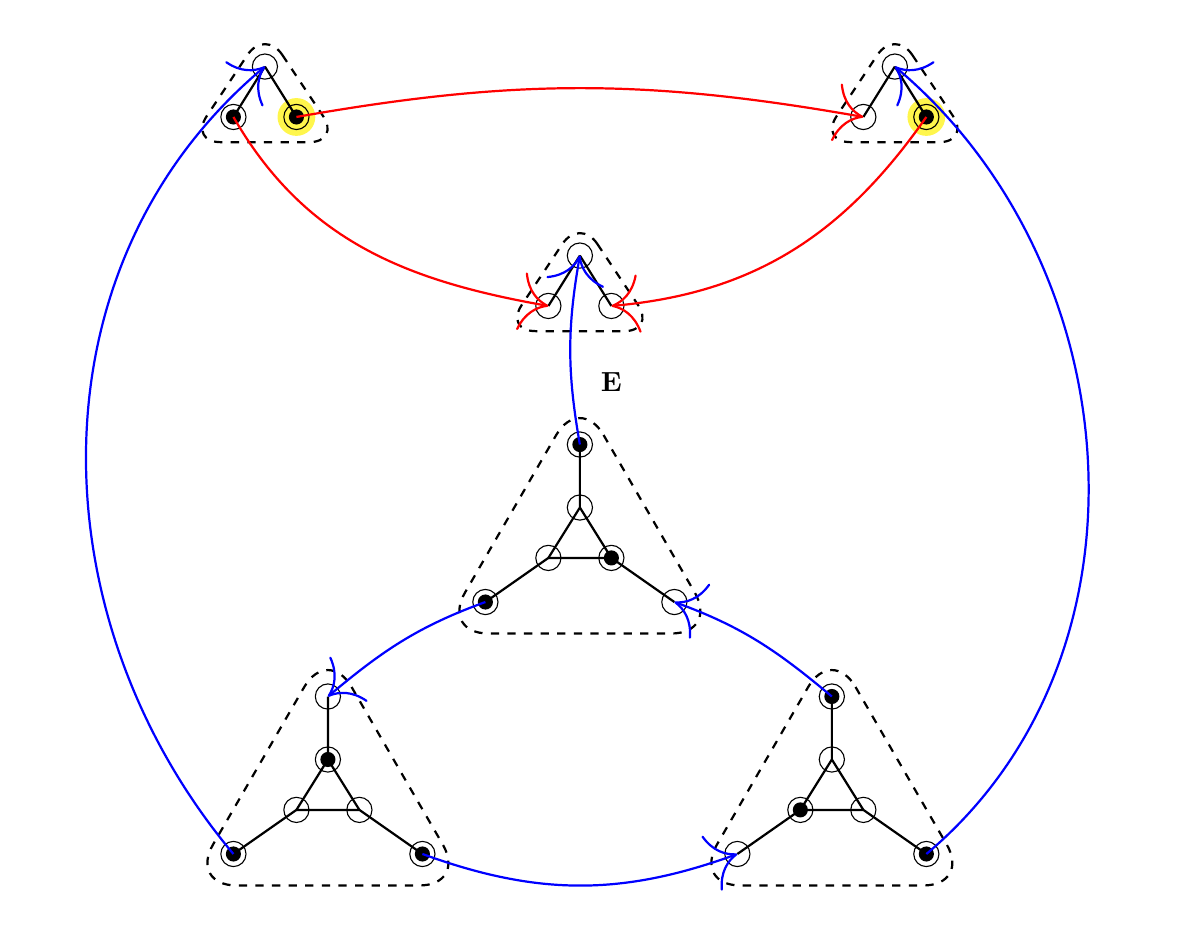
\begin{tikzpicture}[scale=0.8]
        %%%%%%%%%%%% AND 1 %%%%%%%%%%%%
        \def\ver{0.12} %size of a vertex
        \def\xa{-1}
        \def\ya{0}
        % Highlight change
        \draw[fill=yellow, opacity=.7, draw=none] (\xa+0.5,\ya-0.8) circle (0.3cm);
        %\draw[fill=yellow, opacity=.7, draw=none] (\xa-0.5,\ya-0.8) circle (0.3cm);
        %graph G
        \draw (\xa,\ya) circle (0.2cm);          %v1 no fill
        \draw (\xa+0.5,\ya-0.8) circle (0.2cm);  %v4 no fill
        \draw (\xa-0.5,\ya-0.8) circle (0.2cm);  %v3 no fill
        % Tokens
        \path[fill] (\xa-0.5,\ya-0.8) circle (\ver);   %v3
        \path[fill] (\xa+0.5,\ya-0.8) circle (\ver);   %v4
        %labels
        \draw[thick] (\xa,\ya)--(\xa-0.5,\ya-0.8);
        \draw[thick] (\xa,\ya)--(\xa+0.5,\ya-0.8);
        \path[draw, thick, dashed, rounded corners=4mm] (\xa,\ya+0.6)--(\xa+1.2,\ya-1.2)--(\xa-1.2,\ya-1.2)--cycle;
        %%%%%%%%%%%% AND 2 %%%%%%%%%%%%
        \def\ver{0.12} %size of a vertex
        \def\xb{4}
        \def\yb{-3}
        %graph G
        \draw (\xb,\yb) circle (0.2cm);          %v1 no fill
        \draw (\xb+0.5,\yb-0.8) circle (0.2cm);  %v4 no fill
        \draw (\xb-0.5,\yb-0.8) circle (0.2cm);  %v3 no fill
        %labels
        \draw[thick] (\xb,\yb)--(\xb-0.5,\yb-0.8);
        \draw[thick] (\xb,\yb)--(\xb+0.5,\yb-0.8);
        \path[draw, thick, dashed, rounded corners=4mm] (\xb,\yb+0.6)--(\xb+1.2,\yb-1.2)--(\xb-1.2,\yb-1.2)--cycle;
        %%%%%%%%%%%% AND 3 %%%%%%%%%%%%
        \def\ver{0.12} %size of a vertex
        \def\xc{9}
        \def\yc{0}
        % Highlight
        \draw[fill=yellow, opacity=.7, draw=none] (\xc+0.5,\yc-0.8) circle (0.3cm);
        %graph G
        \draw (\xc,\yc) circle (0.2cm);          %v1 no fill
        \draw (\xc+0.5,\yc-0.8) circle (0.2cm);  %v4 no fill
        \draw (\xc-0.5,\yc-0.8) circle (0.2cm);  %v3 no fill
        % Tokens
        \path[fill] (\xc+0.5,\yc-0.8) circle (\ver);   %v4
        %labels
        \draw[thick] (\xc,\yc)--(\xc-0.5,\yc-0.8);
        \draw[thick] (\xc,\yc)--(\xc+0.5,\yc-0.8);
        \path[draw, thick, dashed, rounded corners=4mm] (\xc,\yc+0.6)--(\xc+1.2,\yc-1.2)--(\xc-1.2,\yc-1.2)--cycle;
        %%%%%%%%%%%% OR 1 %%%%%%%%%%%%
        \def\ver{0.12} %size of a vertex
        \def\xd{0}
        \def\yd{-11}
        %G_1
        \draw (\xd,\yd) circle (0.2cm);           %v1
        \draw (\xd+0.5,\yd-0.8) circle (0.2cm);   %v4
        \draw (\xd-0.5,\yd-0.8) circle (0.2cm);   %v3
        \draw (\xd,\yd+1) circle (0.2cm);         %v2
        \draw (\xd-1.5,\yd-1.5) circle (0.2cm);   %v5
        \draw (\xd+1.5,\yd-1.5) circle (0.2cm);   %v6
        % tokens
        \path[fill] (\xd,\yd) circle (\ver);           %v1
        \path[fill] (\xd-1.5,\yd-1.5) circle (\ver);   %v5
        \path[fill] (\xd+1.5,\yd-1.5) circle (\ver);   %v6
        %labels
        \draw[thick] (\xd,\yd+1)--(\xd, \yd)--(\xd-0.5,\yd-0.8)--(\xd-1.5,\yd-1.5);
        \draw[thick] (\xd-0.5,\yd-0.8)--(\xd+0.5,\yd-0.8)--(\xd+1.5,\yd-1.5);
        \draw[thick] (\xd,\yd)-- (\xd+0.5,\yd-0.8);
        %edges
        \path[draw, thick, dashed, rounded corners=6mm] (\xd,\yd+1.8)--(\xd+2.2,\yd-2)--(\xd-2.2,\yd-2)--cycle;
        %%%%%%%%%%%% OR 2 %%%%%%%%%%%%
        \def\ver{0.12} %size of a vertex
        \def\xe{4}
        \def\ye{-7}
        %G_1
        \draw (\xe,\ye) circle (0.2cm);           %v1
        \draw (\xe+0.5,\ye-0.8) circle (0.2cm);   %v4
        \draw (\xe-0.5,\ye-0.8) circle (0.2cm);   %v3
        \draw (\xe,\ye+1) circle (0.2cm);         %v2
        \draw (\xe-1.5,\ye-1.5) circle (0.2cm);   %v5
        \draw (\xe+1.5,\ye-1.5) circle (0.2cm);   %v6
        % token
        \path[fill] (\xe,\ye+1) circle (\ver);         %v2
        \path[fill] (\xe+0.5,\ye-0.8) circle (\ver);   %v4
        \path[fill] (\xe-1.5,\ye-1.5) circle (\ver);   %v5
        %labels
        \draw[thick] (\xe,\ye+1)--(\xe, \ye)--(\xe-0.5,\ye-0.8)--(\xe-1.5,\ye-1.5);
        \draw[thick] (\xe-0.5,\ye-0.8)--(\xe+0.5,\ye-0.8)--(\xe+1.5,\ye-1.5);
        \draw[thick] (\xe,\ye)-- (\xe+0.5,\ye-0.8);

        \path[draw, thick, dashed, rounded corners=6mm] (\xe,\ye+1.8)--(\xe+2.2,\ye-2)--(\xe-2.2,\ye-2)--cycle;

        %%%%%%%%%%%% OR 3 %%%%%%%%%%%%
        \def\ver{0.12} %size of a vertex
        \def\xf{8}
        \def\yf{-11}
        %G_1
        \draw (\xf,\yf) circle (0.2cm);           %v1
        \draw (\xf+0.5,\yf-0.8) circle (0.2cm);   %v4
        \draw (\xf-0.5,\yf-0.8) circle (0.2cm);   %v3
        \draw (\xf,\yf+1) circle (0.2cm);         %v2
        \draw (\xf-1.5,\yf-1.5) circle (0.2cm);   %v5
        \draw (\xf+1.5,\yf-1.5) circle (0.2cm);   %v6

        \path[fill] (\xf,\yf+1) circle (\ver);         %v2
        \path[fill] (\xf-0.5,\yf-0.8) circle (\ver);   %v3
        \path[fill] (\xf+1.5,\yf-1.5) circle (\ver);   %v6
        %labels
        \draw[thick] (\xf,\yf+1)--(\xf, \yf)--(\xf-0.5,\yf-0.8)--(\xf-1.5,\yf-1.5);
        \draw[thick] (\xf-0.5,\yf-0.8)--(\xf+0.5,\yf-0.8)--(\xf+1.5,\yf-1.5);
        \draw[thick] (\xf,\yf)-- (\xf+0.5,\yf-0.8);

        \path[draw, thick, dashed, rounded corners=6mm] (\xf,\yf+1.8)--(\xf+2.2,\yf-2)--(\xf-2.2,\yf-2)--cycle;
        %%%%%%%%%%% EDGES %%%%%%%%%
        \node (a) at (4.5,-5) {\textbf{E}};            % Label reject
        \draw [-, red, thick, arrows={->[scale=3,red]}]  (\xa+0.5,\ya-0.8) to [out=10,in=170]  (\xc-0.5,\yc-0.8);          % AND 1  -- AND 3
        \draw [-, red, thick, arrows={->[scale=3,red]}] (\xa-0.5,\ya-0.8)  to [out=300,in=170] (\xb-0.5,\yb-0.8);          % AND 1  -- AND 2
        \draw [-, red, thick, arrows={->[scale=3,red]}] (\xc+0.5,\yc-0.8) to [out=235,in=5] (\xb+0.5,\yb-0.8) ;            % AND 3  -- AND 2
        \draw [-, blue, thick, arrows={->[scale=3,blue]}] (\xd-1.5,\yd-1.5) to [out=130,in=220] (\xa,\ya);                 % OR 1  -- AND 1
        \draw [-, blue, thick, arrows={->[scale=3,blue]}] (\xd+1.5,\yd-1.5) to [out=340,in=200] (\xf-1.5,\yf-1.5);         % OR 1  -- OR 3
        \draw [-, blue, thick, arrows={->[scale=3,blue]}] (\xf,\yf+1)  to [out=140,in=340] (\xe+1.5,\ye-1.5);              % OR 3  -- OR 2
        \draw [-, blue, thick, arrows={->[scale=3,blue]}] (\xe-1.5,\ye-1.5) to [out=200,in=40] (\xd,\yd+1);                % OR 2  -- OR 1
        \draw [-, blue, thick, arrows={->[scale=3,blue]}] (\xf+1.5,\yf-1.5) to [out=40,in=320] (\xc,\yc);                  % OR 3  -- AND 3
        \draw [-, blue, thick, arrows={->[scale=3,blue]}] (\xe,\ye+1) to [out=100,in=260] (\xb,\yb);                       % OR 2  -- AND 2
      \end{tikzpicture}
    \end{scaletikzpicturetowidth}
    \caption{$S_2.$}
    \label{fig:output_instance_final}
  \end{subfigure}
  \vspace{3em}
  \begin{subfigure}[b]{0.6\textwidth}
    \begin{scaletikzpicturetowidth}{\textwidth}
      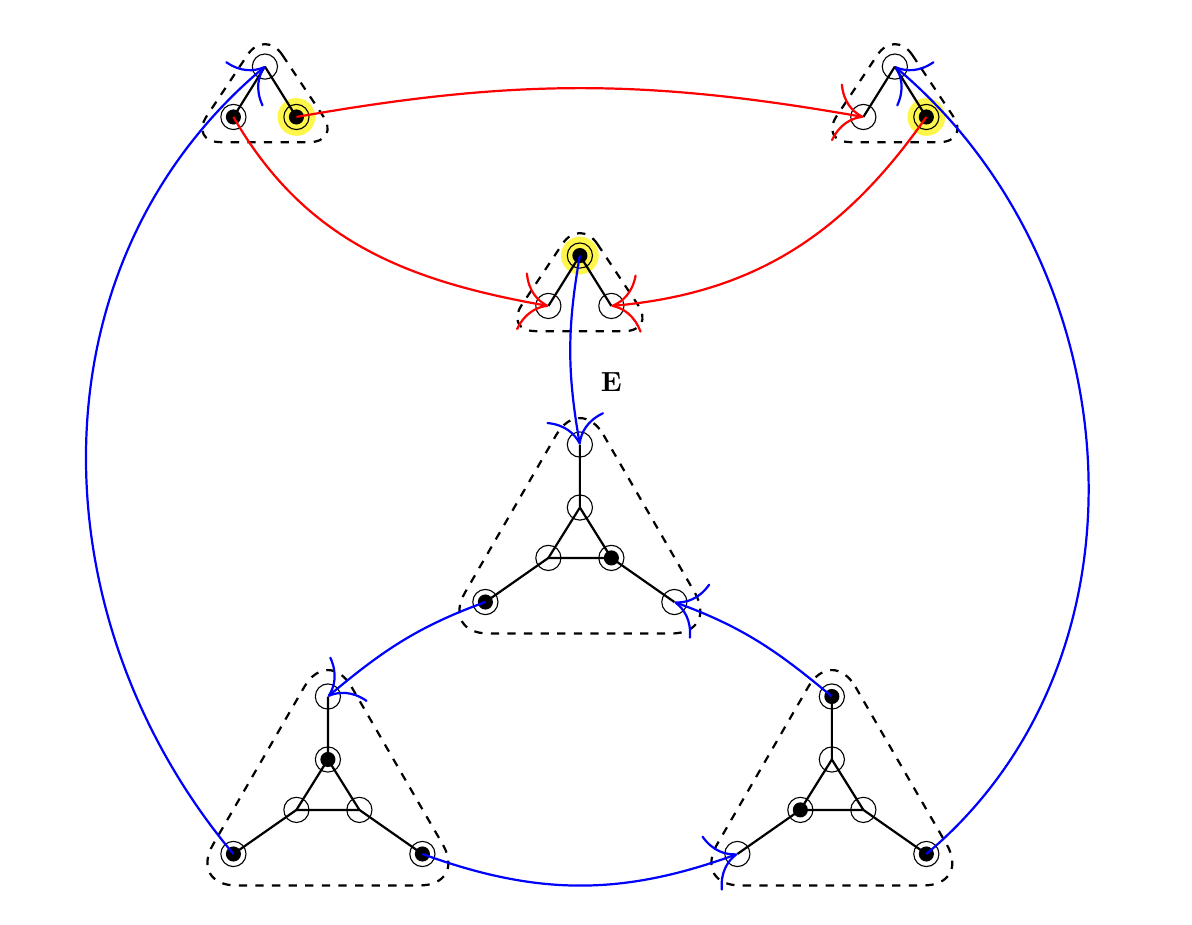
\begin{tikzpicture}[scale=0.8]
        %%%%%%%%%%%% AND 1 %%%%%%%%%%%%
        \def\ver{0.12} %size of a vertex
        \def\xa{-1}
        \def\ya{0}
        % Highlight change
        \draw[fill=yellow, opacity=.7, draw=none] (\xa+0.5,\ya-0.8) circle (0.3cm);
        %\draw[fill=yellow, opacity=.7, draw=none] (\xa-0.5,\ya-0.8) circle (0.3cm);
        %graph G
        \draw (\xa,\ya) circle (0.2cm);          %v1 no fill
        \draw (\xa+0.5,\ya-0.8) circle (0.2cm);  %v4 no fill
        \draw (\xa-0.5,\ya-0.8) circle (0.2cm);  %v3 no fill
        % Tokens
        \path[fill] (\xa-0.5,\ya-0.8) circle (\ver);   %v3
        \path[fill] (\xa+0.5,\ya-0.8) circle (\ver);   %v4
        %labels
        \draw[thick] (\xa,\ya)--(\xa-0.5,\ya-0.8);
        \draw[thick] (\xa,\ya)--(\xa+0.5,\ya-0.8);
        \path[draw, thick, dashed, rounded corners=4mm] (\xa,\ya+0.6)--(\xa+1.2,\ya-1.2)--(\xa-1.2,\ya-1.2)--cycle;
        %%%%%%%%%%%% AND 2 %%%%%%%%%%%%
        \def\ver{0.12} %size of a vertex
        \def\xb{4}
        \def\yb{-3}
        % Highlight change
        \draw[fill=yellow, opacity=.7, draw=none] (\xb,\yb) circle (0.3cm);
        %graph G
        \draw (\xb,\yb) circle (0.2cm);          %v1 no fill
        \draw (\xb+0.5,\yb-0.8) circle (0.2cm);  %v4 no fill
        \draw (\xb-0.5,\yb-0.8) circle (0.2cm);  %v3 no fill
        % Tokens
        \path[fill] (\xb,\yb)  circle (\ver);   %v1
        %labels
        \draw[thick] (\xb,\yb)--(\xb-0.5,\yb-0.8);
        \draw[thick] (\xb,\yb)--(\xb+0.5,\yb-0.8);
        \path[draw, thick, dashed, rounded corners=4mm] (\xb,\yb+0.6)--(\xb+1.2,\yb-1.2)--(\xb-1.2,\yb-1.2)--cycle;
        %%%%%%%%%%%% AND 3 %%%%%%%%%%%%
        \def\ver{0.12} %size of a vertex
        \def\xc{9}
        \def\yc{0}
        % Highlight
        \draw[fill=yellow, opacity=.7, draw=none] (\xc+0.5,\yc-0.8) circle (0.3cm);
        %graph G
        \draw (\xc,\yc) circle (0.2cm);          %v1 no fill
        \draw (\xc+0.5,\yc-0.8) circle (0.2cm);  %v4 no fill
        \draw (\xc-0.5,\yc-0.8) circle (0.2cm);  %v3 no fill
        % Tokens
        \path[fill] (\xc+0.5,\yc-0.8) circle (\ver);   %v4
        %labels
        \draw[thick] (\xc,\yc)--(\xc-0.5,\yc-0.8);
        \draw[thick] (\xc,\yc)--(\xc+0.5,\yc-0.8);
        \path[draw, thick, dashed, rounded corners=4mm] (\xc,\yc+0.6)--(\xc+1.2,\yc-1.2)--(\xc-1.2,\yc-1.2)--cycle;
        %%%%%%%%%%%% OR 1 %%%%%%%%%%%%
        \def\ver{0.12} %size of a vertex
        \def\xd{0}
        \def\yd{-11}
        %G_1
        \draw (\xd,\yd) circle (0.2cm);           %v1
        \draw (\xd+0.5,\yd-0.8) circle (0.2cm);   %v4
        \draw (\xd-0.5,\yd-0.8) circle (0.2cm);   %v3
        \draw (\xd,\yd+1) circle (0.2cm);         %v2
        \draw (\xd-1.5,\yd-1.5) circle (0.2cm);   %v5
        \draw (\xd+1.5,\yd-1.5) circle (0.2cm);   %v6

        \path[fill] (\xd,\yd) circle (\ver);           %v1
        \path[fill] (\xd-1.5,\yd-1.5) circle (\ver);   %v5
        \path[fill] (\xd+1.5,\yd-1.5) circle (\ver);   %v6
        %labels
        \draw[thick] (\xd,\yd+1)--(\xd, \yd)--(\xd-0.5,\yd-0.8)--(\xd-1.5,\yd-1.5);
        \draw[thick] (\xd-0.5,\yd-0.8)--(\xd+0.5,\yd-0.8)--(\xd+1.5,\yd-1.5);
        \draw[thick] (\xd,\yd)-- (\xd+0.5,\yd-0.8);

        \path[draw, thick, dashed, rounded corners=6mm] (\xd,\yd+1.8)--(\xd+2.2,\yd-2)--(\xd-2.2,\yd-2)--cycle;

        %%%%%%%%%%%% OR 2 %%%%%%%%%%%%
        \def\ver{0.12} %size of a vertex
        \def\xe{4}
        \def\ye{-7}
        %G_1
        \draw (\xe,\ye) circle (0.2cm);           %v1
        \draw (\xe+0.5,\ye-0.8) circle (0.2cm);   %v4
        \draw (\xe-0.5,\ye-0.8) circle (0.2cm);   %v3
        \draw (\xe,\ye+1) circle (0.2cm);         %v2
        \draw (\xe-1.5,\ye-1.5) circle (0.2cm);   %v5
        \draw (\xe+1.5,\ye-1.5) circle (0.2cm);   %v6

        \path[fill] (\xe+0.5,\ye-0.8) circle (\ver);   %v4
        \path[fill] (\xe-1.5,\ye-1.5) circle (\ver);   %v5
        %labels
        \draw[thick] (\xe,\ye+1)--(\xe, \ye)--(\xe-0.5,\ye-0.8)--(\xe-1.5,\ye-1.5);
        \draw[thick] (\xe-0.5,\ye-0.8)--(\xe+0.5,\ye-0.8)--(\xe+1.5,\ye-1.5);
        \draw[thick] (\xe,\ye)-- (\xe+0.5,\ye-0.8);

        \path[draw, thick, dashed, rounded corners=6mm] (\xe,\ye+1.8)--(\xe+2.2,\ye-2)--(\xe-2.2,\ye-2)--cycle;

        %%%%%%%%%%%% OR 3 %%%%%%%%%%%%
        \def\ver{0.12} %size of a vertex
        \def\xf{8}
        \def\yf{-11}
        %G_1
        \draw (\xf,\yf) circle (0.2cm);           %v1
        \draw (\xf+0.5,\yf-0.8) circle (0.2cm);   %v4
        \draw (\xf-0.5,\yf-0.8) circle (0.2cm);   %v3
        \draw (\xf,\yf+1) circle (0.2cm);         %v2
        \draw (\xf-1.5,\yf-1.5) circle (0.2cm);   %v5
        \draw (\xf+1.5,\yf-1.5) circle (0.2cm);   %v6

        \path[fill] (\xf,\yf+1) circle (\ver);         %v2
        \path[fill] (\xf-0.5,\yf-0.8) circle (\ver);   %v3
        \path[fill] (\xf+1.5,\yf-1.5) circle (\ver);   %v6
        %labels
        \draw[thick] (\xf,\yf+1)--(\xf, \yf)--(\xf-0.5,\yf-0.8)--(\xf-1.5,\yf-1.5);
        \draw[thick] (\xf-0.5,\yf-0.8)--(\xf+0.5,\yf-0.8)--(\xf+1.5,\yf-1.5);
        \draw[thick] (\xf,\yf)-- (\xf+0.5,\yf-0.8);

        \path[draw, thick, dashed, rounded corners=6mm] (\xf,\yf+1.8)--(\xf+2.2,\yf-2)--(\xf-2.2,\yf-2)--cycle;

        %%%%%%%%%%% EDGES %%%%%%%%%
        \node (a) at (4.5,-5) {\textbf{E}};            % Label reject
        \draw [-, red, thick, arrows={->[scale=3,red]}]  (\xa+0.5,\ya-0.8) to [out=10,in=170]  (\xc-0.5,\yc-0.8);          % AND 1  -- AND 3
        \draw [-, red, thick, arrows={->[scale=3,red]}] (\xa-0.5,\ya-0.8)  to [out=300,in=170] (\xb-0.5,\yb-0.8);          % AND 1  -- AND 2
        \draw [-, red, thick, arrows={->[scale=3,red]}] (\xc+0.5,\yc-0.8) to [out=235,in=5] (\xb+0.5,\yb-0.8) ;            % AND 3  -- AND 2
        \draw [-, blue, thick, arrows={->[scale=3,blue]}] (\xd-1.5,\yd-1.5) to [out=130,in=220] (\xa,\ya);                 % OR 1  -- AND 1
        \draw [-, blue, thick, arrows={->[scale=3,blue]}] (\xd+1.5,\yd-1.5) to [out=340,in=200] (\xf-1.5,\yf-1.5);         % OR 1  -- OR 3
        \draw [-, blue, thick, arrows={->[scale=3,blue]}] (\xf,\yf+1)  to [out=140,in=340] (\xe+1.5,\ye-1.5);              % OR 3  -- OR 2
        \draw [-, blue, thick, arrows={->[scale=3,blue]}] (\xe-1.5,\ye-1.5) to [out=200,in=40] (\xd,\yd+1);                % OR 2  -- OR 1
        \draw [-, blue, thick, arrows={->[scale=3,blue]}] (\xf+1.5,\yf-1.5) to [out=40,in=320] (\xc,\yc);                  % OR 3  -- AND 3
        \draw [-, blue, thick, arrows={->[scale=3,blue]}] (\xb,\yb) to [out=260,in=100] (\xe,\ye+1);                       % AND 2  -- OR 2
      \end{tikzpicture}
    \end{scaletikzpicturetowidth}
    \caption{$S_3.$}
    \label{fig:output_instance_final}
  \end{subfigure}
\caption{Reconfiguration sequence which transforms the initial configuration $S_0$ of the corresponding output sliding token instance to the target configuration $S_3$.}
\label{fig:input_instance_config_to_edge}
\end{figure}
\end{example}


\section{Labelled variant of Sliding-Token Problem}\label{sec:labelled_sliding_token}

The labelled sliding token problem is a variant of the Sliding token problem where each token has a unique label. The purpose of this section is
to prove that the sliding token problem remains $\PSPACE$-hard even with labelled tokens. In \cite{bonsma}, Bonsma showed that a slightly different
version of the SLIDING TOKEN problem is also $\PSPACE$-hard. This latter version called the Standard sliding token problem
(described in section \ref{subsec:standard_sliding_token}) is then used to establish the hardness of the $k$-COLOUR PATH problem. To achieve our
goal only a slight modification of that proof is needed. For the sake of completeness we will go through the original proof and add the
modification needed. On our journey we will encouter some interesting graph colouring problems described in sections \ref{subsection:coloring_problems}.

\subsection{Standard sliding token problem}\label{subsec:standard_sliding_token}
Bonsma and Cereceda showed in \cite{bonsma} that the sliding tokens problem remains $\PSPACE$-complete even for very restricted graphs and
token configurations, defined as follows : The graph $G_s$ is composed of \textit{token triangles} (i.e., copies of $K_3$), \textit{token edges}
(i.e., copies of $K_2$) and link edges. Every vertex of $G_s$ is part of exactly one token triangle or one token edge.
Token triangles and token edges are all mutually disjoint, and joined together by link edges. Moreover, each vertex in a token triangle is of
degree exactly $3$, and $G_s$ has a planar embedding such that every token triangle forms a face. Thus, The maximum degree of $G_s$ is $3$
and minimum degree is $2$. An instance of the Standard Sliding token problem is shown in figure \ref{fig:standard_sliding}.

\begin{figure}[H]
  \centering
    \begin{scaletikzpicturetowidth}{\textwidth}
      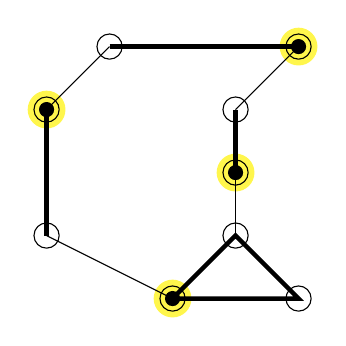
\begin{tikzpicture}[scale=0.8]
        \def\ver{0.12} %size of a vertex
        \def\xa{0}
        \def\ya{0}
        % Highlight change
        \draw[fill=yellow, opacity=.7, draw=none] (\xa-1,\ya-1)  circle (0.3cm);
        \draw[fill=yellow, opacity=.7, draw=none] (\xa-3,\ya+2) circle (0.3cm);
        \draw[fill=yellow, opacity=.7, draw=none] (\xa+1,\ya+3)  circle (0.3cm);
        \draw[fill=yellow, opacity=.7, draw=none] (\xa,\ya+1)  circle (0.3cm);

        %graph G
        \draw (\xa,\ya) circle (0.2cm);          % t11 no fill
        \draw (\xa+1,\ya-1) circle (0.2cm);      % t12 no fill
        \draw (\xa-1,\ya-1) circle (0.2cm);      % t13 no fill
        \draw (\xa-3,\ya) circle (0.2cm);        % e11 no fill
        \draw (\xa-3,\ya+2) circle (0.2cm);      % e12 no fill
        \draw (\xa-2,\ya+3) circle (0.2cm);      % e21 no fill
        \draw (\xa+1,\ya+3) circle (0.2cm);      % e22 no fill
        \draw (\xa,\ya+2) circle (0.2cm);        % e31 no fill
        \draw (\xa,\ya+1) circle (0.2cm);        % e32 no fill

        % Tokens
        \path[fill] (\xa-1,\ya-1) circle (\ver);   % t13
        \path[fill] (\xa-3,\ya+2) circle (\ver);   % e12
        \path[fill] (\xa+1,\ya+3) circle (\ver);   % e22
        \path[fill] (\xa,\ya+1) circle (\ver);     % e32

        % edges
        \draw[ultra thick] (\xa,\ya)--(\xa+1,\ya-1)--(\xa-1,\ya-1)--cycle;
        \draw[ultra thick] (\xa-3,\ya)--(\xa-3,\ya+2) ;
        \draw[ultra thick] (\xa-2,\ya+3)--(\xa+1,\ya+3) ;
        \draw[ultra thick] (\xa,\ya+2)--(\xa,\ya+1) ;

        \draw (\xa-2,\ya+3)--(\xa-3,\ya+2);
        \draw (\xa-3,\ya)--(\xa-1,\ya-1);
        \draw (\xa,\ya+1)--(\xa,\ya);
        \draw (\xa,\ya+2)--(\xa+1,\ya+3);

      \end{tikzpicture}
    \end{scaletikzpicturetowidth}
    \caption{An example of a restricted instance graph $G$ together with a standard token configuration.}
    \label{fig:standard_sliding}
\end{figure}


We say that a token configuration $T$ of $G_s$ is \textit{standard} if each token triangle and token edge of $G_s$ contains exactly one token
in $T$. Then, any move from a standard token configuration results in another standard token configuration since any token will never leave its
token triangle or token edge, and will never slide along a link edge because the first time any token would slide to another triangle or edge,
it would become adjacent to the token belonging to this triangle or edge. So tokens may never slide along a link edge. It is this latter
observation that will allow us to prove the $\PSPACE$-hardness of the labelled variant while doing only a little modification
in the original proof.

The sliding tokens problem remains $\PSPACE$-complete even if $G_s$ is such a restricted graph and both $T_0$ and $T_t$ are standard token
configurations \cite{bonsma}. This restricted problem is called the Standard sliding tokens problem.

\subsection{Labelled tokens} \label{subsection:coloring_problems}
Two prominent vertex coulouring problems that we will encounter and are part of the hardness proof of the labelled sliding token problem
are defined hereunder :

\subsubsection{$k$-colouring.}
For a positive integer $k$ and a graph $G$, we define the $k$-colour graph of $G$, denoted $\mathcal{C}_{k}(G)$,
as the graph that has the $k$-colourings of $G$ as its node set, with two $k$-colourings joined by an edge in $\mathcal{C}_{k}(G)$ if they differ
in colour on just one vertex of $G$. The $k$-COLOUR PATH is then defined as follows :
\begin{flushleft}
  k-COLOUR PATH \\
  \textbf{Instance: } Graph $G$, two $k$-colourings of $G, \alpha$ and $\beta$. \\
  \textbf{Question: } Is there a path between $\alpha$ and $\beta$ in $\mathcal{C}_{k}(G)$ ? \\
\end{flushleft}

\subsubsection{List colouring}
Suppose that we are given a graph $G=(V,E)$, and for each vertex of $G$, a list of colours permitted at that particular vertex.
In this context, the LIST-COLOUR PATH is defined as follows :
\begin{flushleft}
  LIST-COLOUR PATH \\
  \textbf{Instance: } Graph $G$, colour lists $L(v) \subseteq \{1,2,3,4\} \forall v \in V(G)$, two list-colourings $\alpha$ and $\beta$. \\
  \textbf{Question: } Is there a path between $\alpha$ and $\beta$ in $\mathcal{C}(G,L)$ ? \\
\end{flushleft}

An interesting relationship between the COLOUR-PATH problem and $k$-COLOUR PATH problem given by Bonsma is defined in lemma \ref{lemma:k_colour_to_list}.
\begin{lemma}\cite{bonsma}\label{lemma:k_colour_to_list}
For any $k \geq 4$, a LIST-COLOUR PATH instance $G, L, \alpha, \beta$ with lists $L(v) \subseteq \{1, 2, 3, 4\}$ can be transformed
into a $k$-COLOUR PATH instance $G^{'}, \alpha^{'}, \beta^{'}$ such that the distance between $\alpha$ and $\beta$ in $\mathcal{C}(G, L)$
(possibly infinite) is the same as the distance between $\alpha^{'}$ and $\beta^{'}$ in $\mathcal{C}_k(G^{'})$.
\end{lemma}

In \cite{bonsma}, Bonsma established that $k$-Colour Path is $\PSPACE$-complete for several graph classes and values of $k \geq 4$.
This result was obtained through a reduction from the Standard Sliding Token problem and done in two steps. First from the Standard
sliding token problem to the LIST-COLOUR path problem and then from the LIST-COLOUR path problem to the $k$-COLOUR path through lemma
\ref{lemma:k_colour_to_list}. In the following sections we will show that the hardness result remains even when the tokens in the
Standard sliding token instance are attributed unique labels.

\subsection{Preliminaries}
\paragraph{(a,b)-forbidding paths} For $a, b \in \{1, \dots, 4\}$,  an $(a, b)$-forbidding path from vertex $u$ to vertex $v$ is a
$(u, v)$-path with colour lists $L$, with $L(u), L(v) \neq \{1, 2, 3, 4\}$, such that in any colouring, it is not possible that
$u$ has colour $a$ and $v$ simultaneously has colour $b$ (please refer to \cite{bonsma} for the formal definition of (a,b)-forbidding paths).


\subsection{Reduction Structure}
Given a restricted instance $G, T_{A}, T_{B}, T$ of the Standard Sliding Token problem where $T$ is a set of labelled token (an example is
shown in figure \ref{fig:input_instance_standard}), we construct an instance $G^{'}, L, \alpha, \beta, T$ of LIST-COLOUR Path such that
standard token configurations of $G$ correspond to list-colourings of $G^{'}$ , and sliding a token in $G$ corresponds to a
sequence of vertex recolourings in $G^{'}$.

We first start by labelling the vertices of $G$: 
\begin{enumerate}
  \item The token triangles are labelled $1, \dots , n_{t}$ , and the vertices of each triangle $i$ are labelled
        $t_{i1}$, $t_{i2}$ and $t_{i3}$.
  \item The token edges are labelled $1, \dots , n_{e}$, and the vertices of each token edge $i$ are labelled
        $e_{i1}$ and $e_{i2}$.
\end{enumerate}

The construction of $G^{'}$ is as follows: For every token triangle $i$ in $G$ we introduce a vertex $t_{i}$, with colour list
$L(t_{i}) = \{1, 2, 3\}$ in $G^{'}$ . For every token edge $i$ in $G$ we introduce a vertex $e_{i}$ in $G^{'}$, with colour
list $L(e_{i}) = \{1, 2\}$. Whenever a link edge of $G$ joins a vertex $t_{ia}$ with a vertex $e_{jb}$, we add an $(a, b)$-forbidding
path of even length between $t_{i}$ and $e_{j}$ in $G$ . We do the same for pairs $t_{ia}$ and $t_{jb}$, and pairs $e_{ia}$ and $e_{jb}$.
Linking the vertices in $G^{'}$ through $(a, b)$-forbidding paths will make sure that no tokens are adjacent to each other (an example is
shown in figure \ref{fig:output_instance_standard}). Note that this is a polynomial-time transformation.

Standard token configurations of $G$ now correspond to colourings of $G^{'}$ as follows:
\begin{enumerate}
  \item For each token edge $i$ of the token configuration, the token being on $e_{ij} (j = 1, 2 )$
  corresponds to colourings of $G$ where $e_{i}$ has colour $j$.
  \item For each token triangle $i$ of the token configuration, the token being on $t_{ij} (j = 1, 2, 3)$,
  corresponds to colourings where $t_{i}$ has colour $j$.
\end{enumerate}

Since tokens are not adjacent, it is possible to choose colours for the internal vertices of the $(a, b)$-forbidding paths so as to
obtain a proper colouring of $G^{'}$. Two colourings $\alpha$ and $\beta$ corresponding to $T_{A}$ and $T_{B}$ respectively are constructed
this way. Note that to a given standard token configuration of $G$ there can correspond multiple colourings of $G$ because of the freedom
in choice of colours for the internal vertices of the $(a, b)$-forbidding paths.

For the labels, let $W$ be the set of token edges and token triangles of $G$ i.e., $W = \{e_1,\dots, e_{|E|} \} \cup \{t_1,\dots, t_{|T|} \}$
where $|E|$ is the total number of edge tokens in $G$ and $|T|$ is the total number of triangle tokens in $G$
and $f: T \rightarrow W$, a function mapping the set of given labels to the tokens on token edges and token triangles of $G$.

\begin{claim} Let $G, T_A, T_B$ be a restricted instance of Sliding Tokens where each token is given a unique label as described in
section \ref{sec:labelled_sliding_token}, and let $G , L, \alpha, \beta$ be the corresponding instance of List-Colour Path as constructed above.
Then $G, T_A, T_B$ is a Yes-instance if and only if $G , L, \alpha, \beta$ is a YES-instance.
\end{claim}\label{theorem:labelled_sliding}

\begin{proof} \cite{bonsma}
Recall that a token configuration in which the token of token edge $i$ (token triangle $i$) is on $e_{ij}$ (on $t_ {ij}$) corresponds
to multiple colourings of $G$ where $ei$ ($t_i$) has colour $j$. Because of this multiplicity of colourings, we define colour classes of
colourings: if two colourings $\kappa$ and $\lambda$ of $G$ have $\kappa(t_i) = \lambda(t_i)$ and $\kappa(e_i) = \lambda(e_i)$ for every $i$,
then $\kappa$ and $\lambda$ are said to be in the same colour class.

Hence the correspondence between standard token configurations and colourings defines a mapping between standard
token configurations and colour classes. This mapping is in fact a bijection: $(a, b)$-forbidding paths restrict their end vertices
from having colours $a$ and $b$ respectively, but they pose no other restriction on the possible colours of their end vertices.
So $t_{ia}$ and $e_{jb}$ cannot both be occupied by a token in a token configuration if and only if no colouring $\kappa$ has $\kappa(t_i)$ = $a$
and $\kappa(e_j) = b$. (Similar statements hold for pairs $t_i$ and $t_j$, and pairs $e_i$ and $e_j$.)

The function $f$ also yields a bijective mapping : Since no token can slide along a link edge in the Standard sliding token,
each element $w \in W$ can be attributed a label such that the colour of $w$ in the output LIST-COULOUR path instance represents
the vertex placement of the label $t \in T$ s.t $f(t) = w$.

Now we claim that if there exists a sequence of moves that transforms $T_A$ into $T_B$, then there exists a sequence of
recolourings that transforms $\alpha$ into $\beta$. We mentioned earlier that any token configuration obtainable from $T_A$ is a standard
token configuration \cite{bonsma}. Hence every token move corresponds to recolouring a vertex $t_i$ or a vertex $e_i$. Note that before
recolouring $t_i$ (or $e_i$), it may be necessary to first recolour some internal vertices of $(a, b)$-forbidding paths incident with
$t_i$ (or $e_i$), but by the definition of $(a, b)$-forbidding paths, we know this is always possible. It can also be seen that when
we finally arrive in the colour class that contains $\beta$ in this way, the internal vertices of all $(a, b)$-forbidding paths can be
recoloured so that exactly the colouring $\beta$ is obtained.

Similarly, for every sequence of recolourings from $\alpha$ to $\beta$ we can construct a sequence of token moves from $T_A$ to $T_B$:
whenever a vertex $t_i$ ($e_i$) is recoloured from colour a to colour $b$, we move the corresponding token from $t_{ia}$ to $t_{ib}$
(from $e_ {ia}$ to $e_{ib}$). This completes the proof.
\end{proof}

\begin{example}{STANDARD SLIDING TOKEN problem to COLOUR-PATH reduction. \\}
  \textbf{Instance instance : STANDARD SLIDING TOKEN instance.} \hfill

\begin{figure}[H]
  \centering
  \begin{subfigure}[b]{0.4\textwidth}
    \begin{scaletikzpicturetowidth}{\textwidth}
      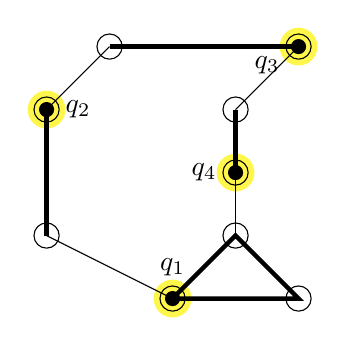
\begin{tikzpicture}[scale=0.8]
        \def\ver{0.12} %size of a vertex
        \def\xa{0}
        \def\ya{0}
        % Highlight change
        \draw[fill=yellow, opacity=.7, draw=none] (\xa-1,\ya-1)  circle (0.3cm);
        \draw[fill=yellow, opacity=.7, draw=none] (\xa-3,\ya+2) circle (0.3cm);
        \draw[fill=yellow, opacity=.7, draw=none] (\xa+1,\ya+3)  circle (0.3cm);
        \draw[fill=yellow, opacity=.7, draw=none] (\xa,\ya+1)  circle (0.3cm);
        %graph G
        \draw (\xa,\ya) circle (0.2cm);          % t11 no fill
        \draw (\xa+1,\ya-1) circle (0.2cm);      % t12 no fill
        \draw (\xa-1,\ya-1) circle (0.2cm);      % t13 no fill
        \draw (\xa-3,\ya) circle (0.2cm);        % e11 no fill
        \draw (\xa-3,\ya+2) circle (0.2cm);      % e12 no fill
        \draw (\xa-2,\ya+3) circle (0.2cm);      % e21 no fill
        \draw (\xa+1,\ya+3) circle (0.2cm);      % e22 no fill
        \draw (\xa,\ya+2) circle (0.2cm);        % e31 no fill
        \draw (\xa,\ya+1) circle (0.2cm);        % e32 no fill
        % Tokens
        \path[fill] (\xa-1,\ya-1) circle (\ver);   % t13
        \path[fill] (\xa-3,\ya+2) circle (\ver);   % e12
        \path[fill] (\xa+1,\ya+3) circle (\ver);   % e22
        \path[fill] (\xa,\ya+1) circle (\ver);     % e32
        % edges
        \draw[ultra thick] (\xa,\ya)--(\xa+1,\ya-1)--(\xa-1,\ya-1)--cycle;
        \draw[ultra thick] (\xa-3,\ya)--(\xa-3,\ya+2) ;
        \draw[ultra thick] (\xa-2,\ya+3)--(\xa+1,\ya+3) ;
        \draw[ultra thick] (\xa,\ya+2)--(\xa,\ya+1) ;
        \draw (\xa-2,\ya+3)--(\xa-3,\ya+2);
        \draw (\xa-3,\ya)--(\xa-1,\ya-1);
        \draw (\xa,\ya+1)--(\xa,\ya);
        \draw (\xa,\ya+2)--(\xa+1,\ya+3);
        % token labels
        \node (l1) at (\xa-1,\ya-0.5) {$q_{1}$};            % Label
        \node (l2) at (\xa-2.5,\ya+2) {$q_{2}$};            % Label
        \node (l3) at (\xa+0.5,\ya+2.7) {$q_{3}$};            % Label
        \node (l4) at (\xa-0.5,\ya+1) {$q_{4}$};            % Label

      \end{tikzpicture}
    \end{scaletikzpicturetowidth}
    \caption{Initial token configuration $T_{A}$.}
    \label{fig:standard_1}
  \end{subfigure}
  \begin{subfigure}[b]{0.4\textwidth}
    \begin{scaletikzpicturetowidth}{\textwidth}
      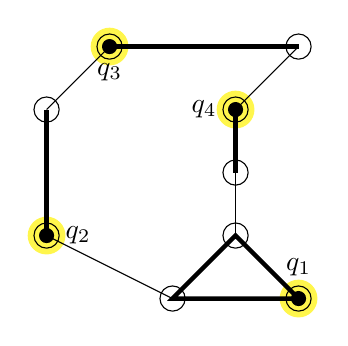
\begin{tikzpicture}[scale=0.8]
        \def\ver{0.12} %size of a vertex
        \def\xa{0}
        \def\ya{0}
        % Highlight change
        \draw[fill=yellow, opacity=.7, draw=none] (\xa+1,\ya-1)  circle (0.3cm);
        \draw[fill=yellow, opacity=.7, draw=none] (\xa-3,\ya) circle (0.3cm);
        \draw[fill=yellow, opacity=.7, draw=none] (\xa-2,\ya+3)  circle (0.3cm);
        \draw[fill=yellow, opacity=.7, draw=none] (\xa,\ya+2)  circle (0.3cm);
        %graph G
        \draw (\xa,\ya) circle (0.2cm);          % t11 no fill
        \draw (\xa+1,\ya-1) circle (0.2cm);      % t12 no fill
        \draw (\xa-1,\ya-1) circle (0.2cm);      % t13 no fill
        \draw (\xa-3,\ya) circle (0.2cm);        % e11 no fill
        \draw (\xa-3,\ya+2) circle (0.2cm);      % e12 no fill
        \draw (\xa-2,\ya+3) circle (0.2cm);      % e21 no fill
        \draw (\xa+1,\ya+3) circle (0.2cm);      % e22 no fill
        \draw (\xa,\ya+2) circle (0.2cm);        % e31 no fill
        \draw (\xa,\ya+1) circle (0.2cm);        % e32 no fill
        % Tokens
        \path[fill] (\xa+1,\ya-1) circle (\ver);   % t12
        \path[fill] (\xa-3,\ya) circle (\ver);     % e11
        \path[fill] (\xa-2,\ya+3) circle (\ver);   % e21
        \path[fill] (\xa,\ya+2) circle (\ver);     % e31
        % edges
        \draw[ultra thick] (\xa,\ya)--(\xa+1,\ya-1)--(\xa-1,\ya-1)--cycle;
        \draw[ultra thick] (\xa-3,\ya)--(\xa-3,\ya+2) ;
        \draw[ultra thick] (\xa-2,\ya+3)--(\xa+1,\ya+3) ;
        \draw[ultra thick] (\xa,\ya+2)--(\xa,\ya+1) ;
        \draw (\xa-2,\ya+3)--(\xa-3,\ya+2);
        \draw (\xa-3,\ya)--(\xa-1,\ya-1);
        \draw (\xa,\ya+1)--(\xa,\ya);
        \draw (\xa,\ya+2)--(\xa+1,\ya+3);
        % token labels
        \node (l1) at (\xa+1,\ya-0.5) {$q_{1}$};            % Label (\xa+1,\ya-1)
        \node (l2) at (\xa-2.5,\ya) {$q_{2}$};            % Label (\xa-3,\ya)
        \node (l3) at (\xa-2,\ya+2.6) {$q_{3}$};            % Label (\xa-2,\ya+3)
        \node (l4) at (\xa-0.5,\ya+2) {$q_{4}$};            % Label (\xa,\ya+2)
      \end{tikzpicture}
    \end{scaletikzpicturetowidth}
    \caption{Target token configuration $T_{B}$.}
    \label{fig:standard_2}
  \end{subfigure}
  \caption{A Standard sliding token instance with initial and target labelled token configuration $T_{A}$ and $T_{B}$ respectively.}
  \label{fig:input_instance_standard}
\end{figure}

% ------------------------- Output instance 1 -----------------------------
  \textbf{Output instance : LIST-COLOUR path instance.} \hfill
\begin{figure}[H]
  \begin{subfigure}[b]{0.9\textwidth}
    \begin{scaletikzpicturetowidth}{\textwidth}
      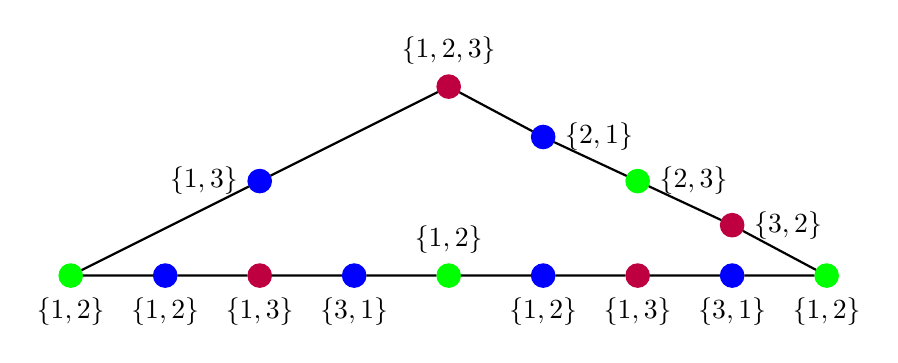
\begin{tikzpicture}[scale=0.8]
        \centering
        \def\ver{0.12} %size of a vertex
        \def\xa{0}
        \def\ya{0}
        \node[Bullet=purple,label=above :{$\{1,2,3\}$}] (t1) at (\xa,\ya+3){};             % t1
        \node[Bullet=blue,label=left :{$\{1,3\}$}] (t11) at (\xa-3,\ya+1.5){};             % t11
        \node[Bullet=blue,label=right:{$\{2,1\}$}] (e33) at (\xa+1.5,\ya+2.2){};           % e33
        \node[Bullet=green,label=right:{$\{2,3\}$}] (e32) at (\xa+3,\ya+1.5){};            % e32
        \node[Bullet=purple,label=right:{$\{3,2\}$}] (e31) at (\xa+4.5,\ya+0.8){};         % e31
        \node[Bullet=green,label=below :{$\{1,2\}$}] (e3) at (\xa+6,\ya){};                % e3
        \node[Bullet=blue,label=below :{$\{3,1\}$}] (e23) at (\xa+4.5,\ya){};              % e23
        \node[Bullet=purple,label=below :{$\{1,3\}$}] (e22) at (\xa+3,\ya){};              % e22
        \node[Bullet=blue,label=below :{$\{1,2\}$}] (e21) at (\xa+1.5,\ya){};              % e21
        \node[Bullet=green,label=above :{$\{1,2\}$}] (e2) at (\xa,\ya){};                  % e2
        \node[Bullet=blue,label=below :{$\{3,1\}$}] (e13) at (\xa-1.5,\ya){};              % e13
        \node[Bullet=purple,label=below :{$\{1,3\}$}] (e12) at (\xa-3,\ya){};              % e12
        \node[Bullet=blue,label=below :{$\{1,2\}$}] (e11) at (\xa-4.5,\ya){};              % e11
        \node[Bullet=green,label=below :{$\{1,2\}$}] (e1) at (\xa-6,\ya){};                % e1

        \draw[thick] (e1)--(e11)--(e12)--(e13)--(e2)--(e21)--(e22)--(e23)--(e3)--(e31)--(e32)--(e33)--(t1)--(t11)--(e1);
      \end{tikzpicture}
    \end{scaletikzpicturetowidth}
    \caption{Initial colouring $\alpha$.}
    \label{fig:list_colour_1}
  \end{subfigure}
  \medskip
  \begin{subfigure}[b]{0.9\textwidth}
    \begin{scaletikzpicturetowidth}{\textwidth}
      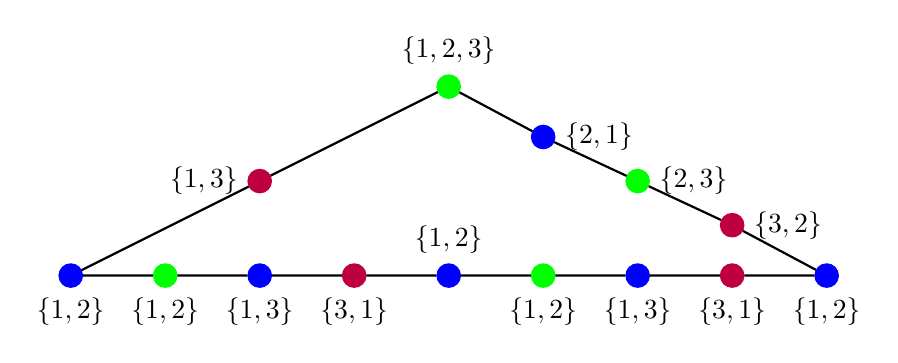
\begin{tikzpicture}[scale=0.8]
        \centering
        \def\ver{0.12} %size of a vertex
        \def\xa{0}
        \def\ya{0}
        \node[Bullet=green,label=above :{$\{1,2,3\}$}] (t1) at (\xa,\ya+3){};             % t1
        \node[Bullet=purple,label=left :{$\{1,3\}$}] (t11) at (\xa-3,\ya+1.5){};          % t11
        \node[Bullet=blue,label=right:{$\{2,1\}$}] (e33) at (\xa+1.5,\ya+2.2){};          % e33
        \node[Bullet=green,label=right:{$\{2,3\}$}] (e32) at (\xa+3,\ya+1.5){};           % e32
        \node[Bullet=purple,label=right:{$\{3,2\}$}] (e31) at (\xa+4.5,\ya+0.8){};        % e31
        \node[Bullet=blue,label=below :{$\{1,2\}$}] (e3) at (\xa+6,\ya){};                % e3
        \node[Bullet=purple,label=below :{$\{3,1\}$}] (e23) at (\xa+4.5,\ya){};           % e23
        \node[Bullet=blue,label=below :{$\{1,3\}$}] (e22) at (\xa+3,\ya){};               % e22
        \node[Bullet=green,label=below :{$\{1,2\}$}] (e21) at (\xa+1.5,\ya){};            % e21
        \node[Bullet=blue,label=above :{$\{1,2\}$}] (e2) at (\xa,\ya){};                  % e2
        \node[Bullet=purple,label=below :{$\{3,1\}$}] (e13) at (\xa-1.5,\ya){};           % e13
        \node[Bullet=blue,label=below :{$\{1,3\}$}] (e12) at (\xa-3,\ya){};               % e12
        \node[Bullet=green,label=below :{$\{1,2\}$}] (e11) at (\xa-4.5,\ya){};            % e11
        \node[Bullet=blue,label=below :{$\{1,2\}$}] (e1) at (\xa-6,\ya){};                % e1

        \draw[thick] (e1)--(e11)--(e12)--(e13)--(e2)--(e21)--(e22)--(e23)--(e3)--(e31)--(e32)--(e33)--(t1)--(t11)--(e1);
      \end{tikzpicture}
    \end{scaletikzpicturetowidth}
    \caption{Target colouring $\beta$}
    \label{fig:list_colour_2}
  \end{subfigure}
  \caption{Output LIST-COLOUR path instance with $\alpha$ being the initial colouring and $\beta$ the target colouring where for better
  visualisation the colour blue is associated to 1, green to 2 and purple to 3 .}
  \label{fig:output_instance_standard}
\end{figure}
\end{example}
\chapter{Reconfiguration of satisfiability problems} \label{chap:SAT}

In this chapter, boolean satisifiability reconfiguration problems are presented. For decades the Boolean satisfiability problem also known
as SAT has fascinated scientific world. In 1978 Schaefer proposed a framework for expressing variants of the satisfiability problem,
and showed a dichotomy theorem: the satisfiability problem for certain classes of Boolean formulas is in $\P$ while it is $\NP$-complete for
all other classes in the framework \cite{schaefer_complexity_1978}. In a single stroke, this result pinpoints the computational complexity
of all well-known variants of SAT, such as $3$-SAT, HORN $3$-SAT, NOT-ALL-EQUAL $3$-SAT, and 1-IN-$3$ SAT \cite{DBLP:journals/siamcomp/GopalanKMP09}.
Since then, dichotomies or trichotomies have been established for several aspects of the satisfiability problem such as optimization
\cite{CREIGNOU1995511,khanna_approximability_2001}, inverse satisfiability \cite{kavvadias_inverse_nodate}, minimal satisfiability \cite{KIROUSIS200320},
and 3-valued satisfiability \cite{10.1145/1120582.1120584}.


Continuing Schaefer's work, Gopalan et al. were interested by the connectivity properties of the solution graph motivated mainly by research
on satisfiability algorithms and the satisfiability threshold. The structure of the solution space of Boolean formulas can be characterized by
a $\textit{solution graph}$ where the vertices are the solutions (satisfying assignments) and two solutions are connection iff they differ in exactly
one variable. The connectivity problem (Conn) is to decide whether the solutions of a given Boolean formula $\varphi$ on $n$ variables induce a
connected subgraph of the $n$-dimensional hypercube, while the st-connectivity problem (st-Conn) is to decide whether two specific
solutions $s$ and $t$ of $\varphi$ are connected. Concerning the st-connectivity question, they proved dichtomies for the diameter of connected components
and the complexity. For the connectivity question, they conjectured a trichotomy. Building on this work, recently the trichotomy was
established by Schwerdtfeger in \cite{schwerdtfeger_computational_2015} and showed that Conn is either in $\P$, $\coNP$-complete, or $\PSPACE$-complete.


Recently, Gopalan et al.'s results have been applied to reconfiguration problems, mostly the st-connectivity and connectivity questions have been
applied to reconfiguration problems such as INDEPENDENT-SET RECONFIGURATION, GRAPH-k-COLORING RECONFIGURATION, and many complexity results were obtained.


\textit{Roadmap.} In section \ref{sec:schaefer's framework} we introduce Schaefer's framework and remarkable results, followed by section
\ref{sec:gopalan-et-al.'s-results} presenting Gopalan et al.'s results. Finally in section \ref{sec:a-computational-trichotomy} we present
Schwerdtfeger's results which establishes the trichotomy conjectured by Gopalan et al.'s for the connectivity problem.


% ----------------------------------------------------------------------------------------------------------------------------------
% ~~~~~~~~~~~~~~~~~~~~~~~~~~~~~~~~~~~~~~~~~~~~~~~~~~~~~~~~~~~~~~~~~~~~~~~~~~~~~~~~~~~~~~~~~~~~~~~~~~~~~~~~~~~~~~~~~~~~~~~~~~~~~~~~~~
% ----------------------------------------------------------------------------------------------------------------------------------
\section{Schaefer's framework}\label{sec:schaefer's framework}
Schaefer identified the complexity of every satisfiability problem SAT($\mathcal{S}$), where $\mathcal{S}$ ranges over all finite sets of
logical relations \cite{schwerdtfeger_computational_2015}. To state Schaefer’s main result, we need to define some basic concepts.
We will use the standard notions and definitions defined in \cite{schaefer_complexity_1978} and \cite{DBLP:journals/siamcomp/GopalanKMP09}.

\subsection{Preliminaries}

A CNF-formula is a Boolean formula of the form $C_{1} \land \dots \land C_{m}$, where each $C_i$ is a finite disjunction of literals where $C_i$
is referred to as a clause. A $k$-CNF formula $(k \geq 1)$ is a CNF-formula where each $C_i$ has at most $k$ literals.


A \textit{logical relation} $R$ is a non-empty subset of $\{0,1\}^n$, for some $n \geq 1$ where $n$ is the \textit{arity} of $R$.
A logical relation is a function that takes as input a Boolean vector and returns a Boolean. For a set $\mathcal{S}$ of logical relations, a
$\mathcal{S}$-formula is a conjuntion of logical relations from $\mathcal{S}$, where the arguments of each relation are freely chosen among
a set of variables.

For a finite set of relations $\mathcal{S}$, a $CNF(\mathcal{S})$-formula over a set of variables $V = \{x_1, \dots, x_n\}$ is a finite
conjunction $C_{1} \land \dots \land C_{m}$, where each $C_i$ is an expression of the form $R(\xi_1,\dots , \xi_k)$, with a $k$-ary
relation $R \in S$, and each $\xi_j$ is a variable from $V$ or one of the constants $0, 1$. A $\textit{solution}$ if a
CNF($\mathcal{S}$)-formula $\varphi$ is an assignment $s = (a_{1}, \dots, a_{n})$ of Boolean values to the variables that makes every
clause of $\varphi$ true. A CNF($\mathcal{S}$)-formula is $\textit{satisfiable}$ if it has at least one solution.

The satisfiability problem SAT($\mathcal{S}$) associated with a finite set $\mathcal{S}$ of logical relations asks:
given a CNF($\mathcal{S}$)-formula $\varphi$, is it satisfiable? All well known restrictions of Boolean satisfiability, such as $3$-SAT,
NOT-ALL-EQUAL $3$-SAT, and POSITIVE $1$-IN-$3$ SAT, can be cast as SAT$(\mathcal{S})$ problems, for a suitable choice of $\mathcal{S}$.

Schaefer identified the complexity of every satisfiability problem SAT($\mathcal{S}$), where $\mathcal{S}$ ranges over all finite sets of
logical relations. To state Schaefer’s main result, we need to define some properties and relations for $R$ and $\mathcal{S}$.

\begin{defn} Let $R$ be a logical relation.
    \begin{enumerate}
        \item $R$ is \textit{bijunctive} if it is the set of solutions of a $2$-CNF formula.
        \item $R$ is \textit{Horn} if it is the set of solutions of a Horn formula, where a Horn formula is a CNF-formula where each $C_i$ has at most
        one positive literal.
        \item $R$ is \textit{dual Horn} if it is the set of solutions of a dual Horn formula, where a dual Horn formula is a CNF-formula where each
        $C_i$ has at most one negative literal.
        \item $R$ is \textit{affine} if it is the set of solutions of a system of linear equations over $\mathcal{Z}_2$.
    \end{enumerate}
\end{defn}

\begin{defn}A set $S$ of logical relations is Schaefer if at least one of the following conditions holds:
    \begin{enumerate}
        \item Every relation in $\mathcal{S}$ is bijunctive.
        \item Every relation in $\mathcal{S}$ is Horn.
        \item Every relation in $\mathcal{S}$ is dual Horn.
        \item Every relation in $\mathcal{S}$ is affine.
    \end{enumerate}
\end{defn}

We are now ready to present Schaefer's theorem :
\begin{theorem}{(Schaefer’s Dichotomy Theorem \cite{schaefer_complexity_1978})} Let $S$ be a finite set of logical relations. If $\mathcal{S}$ is Schaefer, then
SAT($\mathcal{S}$) is in $\P$; otherwise, SAT($\mathcal{S}$) is $\NP$-complete.
\end{theorem}\label{theorem:dichotomy}

Theorem \ref{theorem:dichotomy} is called a dichotomy theorem because Ladner \cite{ladner} has shown that if $\P \neq \NP$, then there are problems
in $\NP$ that are neither in $\P$, nor $\NP$-complete. Thus, Theorem \ref{theorem:dichotomy} asserts that no SAT($\mathcal{S}$) problem
is a problem of the kind discovered by Ladner.



% ----------------------------------------------------------------------------------------------------------------------------------
% ~~~~~~~~~~~~~~~~~~~~~~~~~~~~~~~~~~~~~~~~~~~~~~~~~~~~~~~~~~~~~~~~~~~~~~~~~~~~~~~~~~~~~~~~~~~~~~~~~~~~~~~~~~~~~~~~~~~~~~~~~~~~~~~~~~
% ----------------------------------------------------------------------------------------------------------------------------------
\section{Gopalan et al.'s results}\label{sec:gopalan-et-al.'s-results}

Gopalan et al. continued expanding Schaefer's dichotomie and focused on the connectivity of Boolean satisfiability. They believed
that the connectivity properties of Boolean satisfiability merit some study in their own right, as they shed light on the structure of the solution
space of Boolean formulas thus specifically addressed CNF($\mathcal{S}$)-formulas and studied the complexity of the
following two decision problems,
\begin{itemize}
    \item the connectivity problem $Conn(S)$, that asks for a given $CNF(S)$-formula $\varphi$ whether $G(\varphi)$ is connected,
    \item the st-connectivity problem $st-Conn(S)$, that asks for a given $CNF(S)$-formula $\varphi$ and two solutions $s$ and $t$ whether
    there a path from $s$ to $t$ in $G(\varphi)$.
\end{itemize}

\subsection{Complexity-theoric dichotomies}
Schaefer showed that the satisfiability problem is solvable in polynomial time precisely for formulas built from Boolean
relations all of which are bijunctive, or all of which are Horn, or all of which are dual Horn, or all of which are affine. Gopalan et al.
identified new classes of Boolean relations, called \textit{tight relations}, that properly contain the classes of bijunctive, Horn, dual Horn,
and affine relations. They then showed that st-connectivity is solvable in linear time for formulas built from tight relations,
and $\PSPACE$-complete in all other cases. Their second main result is a dichotomy theorem for the connectivity
problem: it is in $\coNP$ for formulas built from tight relations, and $\PSPACE$-complete in all other cases.

\subsection{Structural dichotomy theorem}
In addition to these two complexity-theoretic dichotomies, they established a structural dichotomy theorem for the diameter of the connected
components of the solution space of Boolean formulas. This result asserts that, in the $\PSPACE$-complete cases, the diameter of
the connected components can be exponential, but in all other cases it is linear. Thus, small
diameter and tractability of the st-connectivity problem are remarkably aligned.

Their results are summarized in comparison to the satisfiability problem SAT($\mathcal{S})$ in table \ref{tab:1}.
\begin{table}[h!]
    \centering
    \begin{tabular}{|c || c | c | c | c |}
        \hline
        $\mathcal{S}$ & SAT($\mathcal{S}$) & ST-CONN($\mathcal{S}$) & CONN($\mathcal{S}$) & Diameter \\ [0.5ex]
        \hline\hline
        Schaefer & $\P$ & $\P$ & $\coNP$ & $O(n)$ \\
        Tight, not Schaefer & $\NP$-compl. & $\P$ & $\coNP$-compl. & $O(n)$ \\
        Not tight & $\NP$-compl. & $\PSPACE$-compl. & $\PSPACE$-compl. & $2^{\Omega (\sqrt{n}) }$ \\ [1ex]
        \hline
    \end{tabular}
    \caption{Gopalan et al.’s results \cite{gopalan_connectivity_2006}}
    \label{tab:1}
\end{table}


\section{A computational Trichotomy for Conn(S)}\label{sec:a-computational-trichotomy}
Schwerdtfeger investigated issues in Gopalan et al.'s work and argued that repeated occurrences of variables in constraint applications
can make the problems harder and the diameter exponential in some cases. This lead to a slight shift of the boundaries established by
Gopalan et al.'s in the hard direction and an introduction to the new classes called \textit{safely tight} and relations \textit{CPSS} fitted to
the correct boundaries.


The following table summarizes their results.
\begin{table}[h!]
    \centering
    \begin{tabular}{|c || c | c | c | c |}
        \hline
        $\mathcal{S}$ & SAT($\mathcal{S}$) & ST-CONN($\mathcal{S}$) & CONN($\mathcal{S}$) & Diameter \\ [0.5ex]
        \hline\hline
        CPSS & $\P$ & $\P$ & $\P$ & $O(n)$ \\
        Schaefer, not CPSS & $\P$ & $\P$ & $\coNP$-compl. & $O(n)$ \\
        Safely tight, not Schaefer & $\NP$-compl. & $\P$ & $\coNP$-compl. & $2^{\Omega (\sqrt{n}) }$ \\
        Not safely tight & $\NP$-compl. & $\PSPACE$-compl. & $\PSPACE$-compl. & $2^{\Omega (\sqrt{n}) }$ \\ [1ex]
        \hline
    \end{tabular}
    \caption{Complete classification of the connectivity problems and the diameter
    for CNF($\mathcal{S}$)-formulas with constants, in comparison to SAT \cite{schwerdtfeger_computational_2015}}
    \label{tab:2}
\end{table}



\chapter{Subset sum Reconfiguration}
The subset sum problem is a well-known \NP-complete problem in which given an integer $x$ and a set of integers $S = \{a_1, a_2,\dots, a_n\}$,
we wish to find a subset $A \subseteq [n]$ such that $\sum_{i \in A} ai = x$ ?

In \cite{Ito11approximabilityof} Ito and Demaine considered the following problem :
Given two packings $A_0$ and $A_t$, both of total size at least $k$, and we are asked whether we can transform one into the other via
packings by moving (namely, either adding or removing) a single item to/from the previous one without ever going through a packing of total size
less than $k$. They called this problem the SUBSET SUM RECONFIGURATION problem and proved that it is strongly $\NP$-hard, and is
$\PSPACE$-complete for the variant with conflict graph.

In this chapter, we explore another reconfiguration version of the subset sum problem referred to as the $k$-move Subset Sum reconfiguration
problem. We say that a set of integers $A_1$ can be \textit{$k$-move reconfigured} into a second set of integers $A_2$ whenever the symmetric
difference of $A_1$ and $A_2$ has cardinality at most $k$. In \cite{cardinal_reconfiguration_2018} the $k$-move Subset Sum reconfiguration
problem was proved to be $\PSPACE$-complete. This chapter is dedicated to that particular proof in an attempt to detail the hardness proof.

\section{$k$-move Subset Sum Reconfiguration}
\begin{defn}{($k$-move Subset Sum Reconfiguration Problem).} Given two solutions $A_1$ and $A_2$ to an instance of the subset sum problem,
can $A_2$ be obtained by repeated $k$-move reconfiguration, beginning with $A_1$, so that all intermediate subsets are also solutions?
\end{defn}

\subsection{Trivial cases}
The reconfiguration problem is trivial if the reconfiguration steps are restricted to involve only the removal or addition of a single element
of $S$, as no single such move can maintain the same sum. The problem remains trivial for $k=2$, since any removed element must be replaced by
itself. For $k=3$, we prove the following theorem:
\begin{theorem}The $3$-move Subset Sum Reconfiguration problem is strongly $\PSPACE$-complete.\end{theorem}

We first start by showing that the $k$-move subset sum problem is in $\PSPACE$ and then provide a $\PSPACE$-hardness proof to show that
it is $\PSPACE$-complete.

\begin{lemma}For every $k \in \mathbb{N}$, the $k$-move Subset Sum Reconfiguration problem is in $\PSPACE$. \end{lemma}
\begin{proof}
For an instance with $|S| = n$, there are $O(n^{k})$ other subsets reachable by a $k-$move reconfiguration, since each such move can be specified
by the set of items in the symmetric difference of the two subsets. So all adjacent subsets in the reconfiguration graph can be enumerated in
polynomial time. Then the $k$-move subset sum reconfiguration  problem is in $\NPSPACE$ by the following algorithm : in the reconfiguration graph,
repeatedly move between subsets by  non-deterministically selecting a neighbour in polynomial time and space. Since \NPSPACE $=$ \PSPACE,
$k$-move subset sum is also in $\PSPACE$.
\end{proof}

\begin{lemma}The $k$-move Subset Sum Reconfiguration problem is $\PSPACE$-hard. \end{lemma}
Proving the hardness is done in two steps. First, reducing the Sliding Token Reconfiguration problem to the Exact Cover Reconfiguration problem.
Then from the Exact Cover Reconfiguration problem to the $3$-move Subset Sum Reconfiguration problem.

\subsubsection{SLIDING TOKEN PROBLEM}
The Sliding token problem is introduced in chapter \ref{chap:NCL} and detailed in section \ref{sec:sliding_tokens}. Hearn and Demaine proved that
the SLIDING TOKEN PROBLEM is $\PSPACE$-complete for planar graphs, as an example of the application of the nondeterministic constraint logic
model and they implicitly proved that the SLIDING TOKEN PROBLEM is $\PSPACE$-hard on $3$-regular graphs since the reduction is done from a
restricted NCL machine (NCL-CONFIGURATION-TO-EDGE) in which the underlying graph is planar and all vertices have degree three. The labeled
variant of the sliding token problem, where each token has a unique label, is also $\PSPACE$-hard and is detailed in section \ref{sec:labeled_sliding_token}
of chapter \ref{chap:NCL} . It is the latter version that is used in the reduction.

\subsubsection{Exact Cover Reconfiguration problem} \label{subsubsection:Exact_cover}
The exact cover reconfiguration problem is the second problem introduced along this reduction.
\begin{defn}{(Exact Cover Split and Merge Reconfiguration).} Given a set $\mathcal{S}$ of subsets of a set $\mathcal{U}$, and two exact covers
$C_1$ and $C_2 \subseteq \mathcal{S}, C_1$ can be reconfigured into $C_2$ via a split (and $C_2$ can be reconfigured into $C_1$ via a merge)
provided that there exist $S_1, S_2, S_3 \subseteq \mathcal{S}$ with $C_1 - C_2 = S_1$ and $C_2 - C_1 = \{s_2, s_3\}$.

Since $C_1, C_2$ are exact covers it is mandatory that $S_1 = S_2 \cup S_3$ and $ S_2 \cap S_3 = \emptyset$.
\end{defn}

\begin{defn}{(Exact Cover Reconfiguration problem).} Given a set $\mathcal{S}$ of subsets of a set $\mathcal{U}$, and two configuration
$C_1$ and $C_2$, can $C_1$ be reconfigured into $C_2$ via repeated splits and merges ?
\end{defn}

\begin{example}
Let $\mathcal{U} = \{1,2,3\}$ and $\mathcal{S} = \{\{1\}, \{2\}, \{3\}, \{1,2\}, \{2,3\}\}$ and the two given configurations be the
following : $C_1 = \{\{1\}, \{2,3\}\}$ and $C_2 = \{\{1,2\}, \{3\}\}$. A solution would be the following :

\begin{figure}[h!]
\begin{center}
\begin{scaletikzpicturetowidth}{\textwidth}
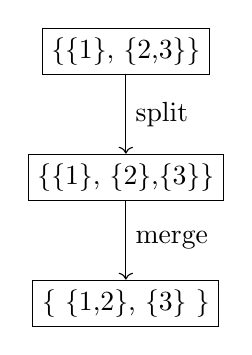
\begin{tikzpicture}[scale=1]
  \node (1) [draw, rectangle] {\{\{1\}, \{2,3\}\}};
  \node (2) [below=of 1, draw, rectangle] {\{\{1\}, \{2\},\{3\}\}};
  \node (3) [below=of 2, draw, rectangle] {\{ \{1,2\}, \{3\} \}};
  \draw[->]  (1) to node [auto] {split} (2);
  \draw[->]  (2) to node [auto] {merge} (3);
\end{tikzpicture}
\end{scaletikzpicturetowidth}
\end{center}
\caption{Reconfiguration sequence which transforms $C_1$ into $C_2$ via splits and merges.}\label{fig:exact_cover}
\end{figure}
\end{example}

\begin{lemma}The Exact Cover Reconfiguration problem is $\PSPACE$-hard for instances that are $23$-colorable hypergraphs. \end{lemma}

\begin{proof}Labeled variant of the SLIDING TOKEN PROBLEM $\leq_p$ Exact Cover Reconfiguration problem.

\subsubsection{Input instance of the Labeled SLIDING TOKEN PROBLEM}
The input instance of the labeled variant of the SLIDING TOKEN PROBLEM is described hereunder.
\begin{itemize}
  \item $G = (V,E)$, a $3$-regular graph.
  \item $T$, a set of labeled tokens.
  \item $p_1 : T \rightarrow V,$ a function mapping each labeled token to a vertex placement in the starting configuration of the output instance.
  \item $p_2 : T \rightarrow V,$ a function mapping each labeled token to a vertex placement in the ending configuration of the output instance.
  \item $I_1 = \{p_1(t) : t \in T\}$ and $I_2 = \{p_2(t) : t \in T\}$ are independent sets of size $|T| \leq |V|$.
\end{itemize}

\begin{example}{Input instance of the Labeled SLIDING TOKEN PROBLEM}
  \begin{figure}[H]
    \begin{center}
      \begin{scaletikzpicturetowidth}{\textwidth}
        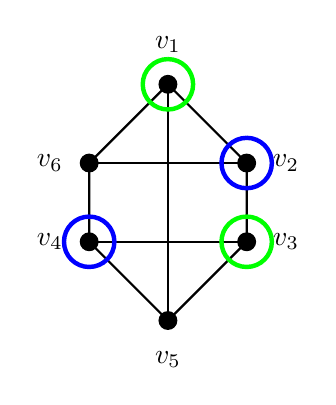
\begin{tikzpicture}[scale=1]

          \def\ver{0.12} %size of a vertex
          \def\xa{1}
          \def\ya{5}
%nodes
          \path[fill] (\xa,\ya) circle (\ver);       % v5
          \path[fill] (\xa+1,\ya+1) circle (\ver);   % v3
          \path[fill] (\xa+1,\ya+2) circle (\ver);   % v2
          \path[fill] (\xa,\ya+3) circle (\ver);     % v1
          \path[fill] (\xa-1,\ya+2) circle (\ver);   % v6
          \path[fill] (\xa-1,\ya+1) circle (\ver);   % v4
%labels
          \node (1) at (\xa,\ya+3.5) {$v_1$};     % v1
          \node (2) at (\xa+1.5,\ya+2) {$v_2$};   % v2
          \node (3) at (\xa+1.5,\ya+1) {$v_3$};   % v3
          \node (5) at (\xa,\ya-0.5) {$v_5$};     % v5
          \node (4) at (\xa-1.5,\ya+1) {$v_4$};   % v4
          \node (6) at (\xa-1.5,\ya+2) {$v_6$};   % v6
%edges
          \draw[thick] (\xa,\ya)--(\xa+1,\ya+1)--(\xa+1,\ya+2)--(\xa,\ya+3)--(\xa-1,\ya+2)--(\xa-1,\ya+1)--(\xa,\ya) ; % contour
          \draw[thick] (\xa,\ya)--(\xa,\ya+3) ;       % v5 - v1
          \draw[thick] (\xa+1,\ya+1)--(\xa-1,\ya+1) ; % v3 - v4
          \draw[thick] (\xa+1,\ya+2)--(\xa-1,\ya+2) ; % v2 - v6
%independent sets
          \draw[ultra thick,green] (\xa,\ya+3+ \ver+0.2) coordinate(a1)  arc (90:450:\ver +0.2) coordinate(a2);
          \draw[ultra thick,green] (\xa+1,\ya+1+ \ver+0.2) coordinate(d1)  arc (90:450:\ver +0.2) coordinate(d2);
          \draw[ultra thick,blue] (\xa-1,\ya+1+ \ver+0.2) coordinate(a1)  arc (90:450:\ver +0.2) coordinate(a2);
          \draw[ultra thick,blue] (\xa+1,\ya+2+ \ver+0.2) coordinate(d1)  arc (90:450:\ver +0.2) coordinate(d2);

        \end{tikzpicture}
      \end{scaletikzpicturetowidth}
    \end{center}
    \caption{}
    \label{fig:input_sliding_token_example}
  \end{figure}
\end{example}

\subsubsection{Preliminaries} \label{sssec:prelim}
\paragraph{Slide Set.}
For each pair of adjacent vertices $v_i, v_j \in V$ of the input instance of the sliding token problem, the set consisting of these two vertices
and their neighbors is called a $slide set$, denoted $S_{i,j}$.
\begin{figure}[H]
\begin{center}
\begin{scaletikzpicturetowidth}{\textwidth}
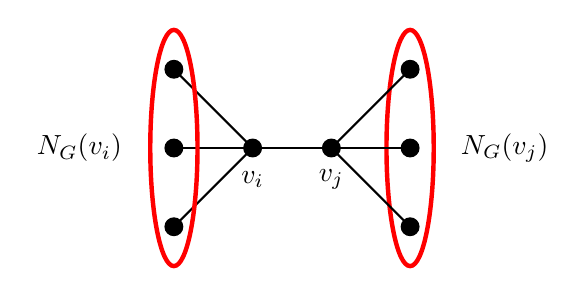
\begin{tikzpicture}[scale=1]
\def\ver{0.12} %size of a vertex
\def\x{1}
\def\xa{1}
\def\ya{0}
\def\xb{2}
%Slide Set
\path[fill] (\xa,\ya) circle (\ver);       % vi
\node (1) at (\xa,\ya-0.4) {$v_i$};
\path[fill] (\xa-1,\ya) circle (\ver);     % v2
\path[fill] (\xa-1,\ya+1) circle (\ver);   % v1
\path[fill] (\xa-1,\ya-1) circle (\ver);   % v3

\draw[thick] (\xa,\ya)--(\xa-1,\ya) ;
\draw[thick] (\xa,\ya)--(\xa-1,\ya+1) ;
\draw[thick] (\xa,\ya)--(\xa-1,\ya-1) ;
\draw[ultra thick, red] (0,0) ellipse (0.3 and 1.5);
\node (3) at (\xa-2.2,\ya) {$N_{G}(v_i)$};
\draw[ultra thick, red] (3,0) ellipse (0.3 and 1.5);
\node (3) at (\xb+2.2,\ya) {$N_{G}(v_j)$};

%graph independent set
\path[fill] (\xb,\ya) circle (\ver);       % v_j
\node (1) at (\xb,\ya-0.4) {$v_j$};
\path[fill] (\xb+1,\ya) circle (\ver);    % v2
\path[fill] (\xb+1,\ya+1) circle (\ver);   % v1
\path[fill] (\xb+1,\ya-1) circle (\ver);   % v3
\draw[thick] (\xb,\ya)--(\xb+1,\ya) ;
\draw[thick] (\xb,\ya)--(\xb+1,\ya+1) ;
\draw[thick] (\xb,\ya)--(\xb+1,\ya-1) ;

\draw[thick] (\xa,\ya)--(\xb,\ya) ;
\end{tikzpicture}
\end{scaletikzpicturetowidth}
\end{center}
\caption{Slide set denoted $S_{ij}$ of vertices $v_i$ and $v_j$.}
\label{fig:slide_set}
\end{figure}

\paragraph{Maximally split configuration $C$.}
A configuration $C$ of the constructed Exact Cover Reconfiguration instance is called \textit{maximally split} if every $c \in C$
contains exactly one vertex and up to one token.

\begin{example}{A maximally split configuration $C$}
  \begin{figure}[h!]
    \begin{center}
      \begin{scaletikzpicturetowidth}{\textwidth}
        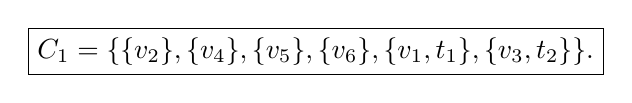
\begin{tikzpicture}[scale=1]
          \node (1) [draw, rectangle] {$C_1 = \{ \{v_2\}, \{v_4\}, \{v_5\}, \{v_6\}, \{v_1, t_1\}, \{v_3, t_2\} \}$.};
        \end{tikzpicture}
      \end{scaletikzpicturetowidth}
    \end{center}
    \caption{A maximally split configuration $C_1$.}
    \label{}
  \end{figure}
  $C_1$ is maximally split since each subset $c \i\in C_1$ contains exactly one vertex and up to one token.
\end{example}

\paragraph{Sploot set of a configuration $C$.}
For each exact cover configuration C in the output instance, let sploot($C$) be the set of all maximally split configurations reachable from $C$.


\subsubsection{Output $\mathcal{U}$ and $\mathcal{S}$}
The output instance of the Exact Cover Reconfiguration problem contains a set $\mathcal{S}$ of subsets of a set $\mathcal{U}$ defined in
\ref{subsubsection:Exact_cover} where :
\begin{itemize}
  \item $\mathcal{U} = \{v_1, v_2, \dots, v_{|V|}\} \cup \{t_1, t_2, \dots, t_{|T|}\}.$
  \item The set $\mathcal{S}$ is defined as follows, for every pair of adjacent vertices $v_i, v_j$ and token $t_k$
    \begin{itemize}
      \item All subsets of $S_{i,j} - \{v_i\}$ and $S_{i,j} - \{v_j\}$.
      \item $\{v_i, t_k\}$ and $\{v_j , t_k\}$.
      \item $S_{i,j} \cup \{t_k\}$.
    \end{itemize}
\end{itemize}

\begin{example}According to the above example, \ref{fig:input_sliding_token_example}, the output instance of the Exact Cover Reconfiguration
problem is the following :
\end{example}

\subsubsection{Output starting and ending configurations, $C_1$ and $C_2$}
The starting configuration $C_1$ is the union of $\{\{ v_i \} : v_i \in V - I_1\}$ and, for every $v_i \in I_1$, a set $\{v_i, t_k\}$ with a
distinct $t_k$.
The ending configuration $C_2$ is then the union of $\{\{ v_i \} : v_i \in V - I_2\}$ and, for every $v_i \in I_2$, a set $\{v_i, t_k\}$ with a
distinct $t_k$.

\begin{example}Continuing the running example, $C_1$ and $C_2$ would be :
\begin{itemize}
  \item $C_1 = \{ \{v_2, v_4, v_5, v_6\}, \{v_1, t_1\}, \{v_3, t_2\}\}$.
  \item $C_2 = \{ \{v_1, v_3, v_5, v_6\}, \{v_2, t_1\}, \{v_4, t_2\}\}$.
\end{itemize}
\end{example}

\subsubsection{$23$-colorability of the output instance $H = (U, \mathcal{S})$}
The goal here is to make sure that no two vertices of distance at most $3$ (i.e. in a common slide set ref \ref{fig:slide_set}) have the same color.
More precisely, we want to prove that given $23$-colours, no two vertices having a common slide set would have the same colour. This constraint
will enforce the absence of tokens on neighbors of $v_i$ and $v_j$, and the presence of a token on $v_i$ or $v_j$, but not both making sure that
any merge or split will result into a feasible configuration. \todo{To check integrity + reformulate}.

Given that the $kth$ power $G^{k}$ of an undirected graph $G$ is another graph that has the same set of vertices, but in which two vertices are
adjacent when their distance in $G$ is at most $k$, to find the colorability of the output instance $H = (U, \mathcal{S})$, it suffices to
compute $\Delta(G^{3})$. Since $G$ is $3-$regular, $G^3$ has degree at most $21$ proven by the following figure where the worst case
scenario ($i.e.,$ a tree is attached to each root so as to force the root to meet new nodes and add new edges).

On veut que dans $\mathcal{S}$, chaque paire de sommet ayant un common slide set n'ait pas la meme couleur.
Pour ce faire on doit connaitre le max deg de $\mathcal{S}$. Pour connaitre le max degrée on va compute le graphe $G^3$ de $G$
car par definition de la kth power d'un graphe $G^3$ sera equivalent $\mathcal{S}$.

\begin{figure} [H]
  \centering
  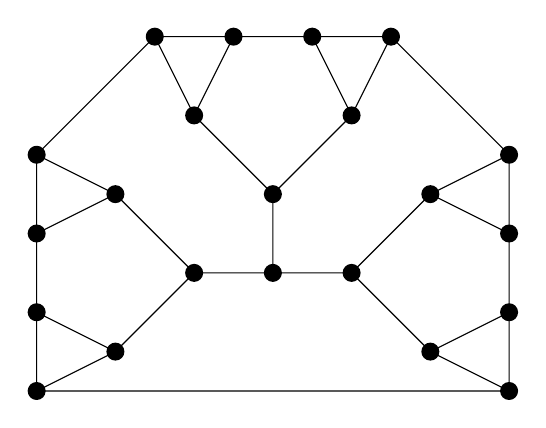
\begin{tikzpicture}
    \def\xa{0}
    \def\ya{0}
    %nodes
    \draw[thick, fill=black] (\xa,\ya) circle (0.1cm);           % v1

    \draw[thick, fill=black] (\xa+1,\ya) circle (0.1cm);         % v2
    \draw[thick, fill=black] (\xa+2,\ya+1) circle (0.1cm);       % v3
    \draw[thick, fill=black] (\xa+2,\ya-1) circle (0.1cm);       % v4
    \draw[thick, fill=black] (\xa+3,\ya-0.5) circle (0.1cm);     % v5
    \draw[thick, fill=black] (\xa+3,\ya-1.5) circle (0.1cm);     % v6
    \draw[thick, fill=black] (\xa+3,\ya+1.5) circle (0.1cm);     % v7
    \draw[thick, fill=black] (\xa+3,\ya+0.5) circle (0.1cm);     % v8

    \draw[thick, fill=black] (\xa,\ya+1) circle (0.1cm);         % v9
    \draw[thick, fill=black] (\xa+1,\ya+2) circle (0.1cm);       % v10
    \draw[thick, fill=black] (\xa-1,\ya+2) circle (0.1cm);       % v11
    \draw[thick, fill=black] (\xa+1.5,\ya+3) circle (0.1cm);     % v12
    \draw[thick, fill=black] (\xa+0.5,\ya+3) circle (0.1cm);     % v13
    \draw[thick, fill=black] (\xa-0.5,\ya+3) circle (0.1cm);     % v14
    \draw[thick, fill=black] (\xa-1.5,\ya+3) circle (0.1cm);     % v15

    \draw[thick, fill=black] (\xa-1,\ya) circle (0.1cm);         % v16
    \draw[thick, fill=black] (\xa-2,\ya+1) circle (0.1cm);       % v17
    \draw[thick, fill=black] (\xa-2,\ya-1) circle (0.1cm);       % v18
    \draw[thick, fill=black] (\xa-3,\ya-1.5) circle (0.1cm);     % v19
    \draw[thick, fill=black] (\xa-3,\ya-0.5) circle (0.1cm);     % v20
    \draw[thick, fill=black] (\xa-3,\ya+0.5) circle (0.1cm);     % v21
    \draw[thick, fill=black] (\xa-3,\ya+1.5) circle (0.1cm);     % v22

    %edges
    \draw (\xa,\ya)--(\xa+1,\ya)--(\xa+2,\ya-1)--(\xa+3,\ya-1.5) ;         % v1 - v2 - v4 - v6
    \draw (\xa+1,\ya)--(\xa+2,\ya+1)--(\xa+3,\ya+1.5) ;                      % v2 - v3 - v7
    \draw (\xa,\ya)--(\xa,\ya+1)--(\xa+1,\ya+2)--(\xa+1.5,\ya+3) ;     % v1 - v9 - v10 - v12
    \draw (\xa,\ya+1)--(\xa-1,\ya+2)--(\xa-1.5,\ya+3) ;            % v9 - v11 - v15
    \draw (\xa,\ya)--(\xa-1,\ya)--(\xa-2,\ya-1)--(\xa-3,\ya-1.5) ;   % v1 - v16 - v18 - v19
    \draw (\xa-1,\ya)--(\xa-2,\ya+1)--(\xa-3,\ya+1.5) ; % v16 - v17 - v22
    \draw (\xa-2,\ya-1)--(\xa-3,\ya-0.5) ; % v18 - v20
    \draw (\xa-2,\ya+1)--(\xa-3,\ya+0.5) ; % v17 - v21
    \draw (\xa-1,\ya+2)--(\xa-0.5,\ya+3) ; % v11 - v14
    \draw (\xa+1,\ya+2)--(\xa+0.5,\ya+3) ; % v10 - v13
    \draw (\xa+2,\ya+1)--(\xa+3,\ya+0.5) ;  % v3 - v8
    \draw (\xa+2,\ya-1)--(\xa+3,\ya-0.5) ; % v4 - v5

    \draw (\xa+3,\ya-1.5)--(\xa-3,\ya-1.5)--(\xa-3,\ya-0.5)--(\xa-3,\ya+0.5)--(\xa-3,\ya+1.5)--(\xa-1.5,\ya+3)--(\xa-0.5,\ya+3)--(\xa+0.5,\ya+3)--(\xa+1.5,\ya+3)--(\xa+3,\ya+1.5)--(\xa+3,\ya+0.5)--(\xa+3,\ya-0.5)--(\xa+3,\ya-1.5)--(\xa-3,\ya-1.5) ; %contour

  \end{tikzpicture}
  \caption{Graph $G^{'}$ (shown darker) is a subgraph of $G$.}
  \label{fig:subgraph}
\end{figure}


So $G$ can be $22-$colored such that no two vertices of distance at most $3$ (i.e. in a common slide set) have the same color. Such a coloring
ensures that no pair of vertices in a common set in $\mathcal{S}$ share a color. Coloring the tokens in $\mathcal{T}$ a distinct (23rd) color
then gives a coloring of $\mathcal{U}$ such that no pair of elements of a common set share the same color.

\subsubsection{High level idea}
We first note that the subsets containing exactly one vertex and a token (e.g., $\{v_i, t_k\}$) represents the presence of the token
$t_k$ on vertex $v_i$ and the subsets consisting of a slide set and a token (e.g., $\{S_{i,j} \cup t_k\}$) represent the presence of a
"mid-slide" token between $v_i$ and $v_j$. A "mid-slide" token can be interpreted as the token $t_k$ not being properly on $v_i$ or $v_j$ but is
"on it's way" from $v_i$ to $v_j$. Therefore, sliding a token $t_k$ from $v_i$ to $v_j$ is simulated by first
merging $\{v_i, t_k\}$ and $S_{i,j}-\{v_i\}$ into $S_{i,j} \cup \{t_k\}$, and then splitting this set into this set into $S_{i,j}-\{v_j\}$
and ${v_j, t_k}$. The first step of this sequence enforces the absence of tokens on neighbors of $v_i$ and $v_j$ since by definition, the slide
set $S_{ij}$ of $v_i$ and $v_j$ contains all the of $v_i$ and $v_j$ and having the token $t_k$  merged in $S_{ij}$ means that $t_k$ is not on any
vertex. The second step then ensures the presence of a token on $v_i$ or $v_j$, but not both.
Before a merge-split sequence, additional splits and merges of token-less sets may be needed to obtain $S_{i,j}-\{v_i\}$.

\subsubsection{Bijection between configurations.}
Given the definition of maximally split configurations in \ref{sssec:prelim}. The following defines a function $f_{red}$ from token arrangements
to maximally split covers in the following way :
\begin{enumerate}
  \item Each token-less vertex corresponds to a set $\{v_i\}$ in the cover.
  \item Each token $t_k$ placed at $v_i$ corresponds to a set $\{v_j, t_k\}$ in the cover.
\end{enumerate}
Notice that $f_{red}$ is a bijection since each cover configuration is an exact cover (pas de doublons) and each token
arrangement contains no doublons no plus. Notice also that $f_{red}(p_1) = C_1$ and $f_{red}(p_2) = C_2$.
\todo{Understand why and how to affirm that it is a bijection + I do not agree with f(p1) = c1 etc}

\subsubsection{Reduction structure.}
The remainder of the proof is devoted to proving the following claim:
\begin{claim} A token arrangement $p^{'}$ is reachable from a token arrangement $p$ if and only if $f_{red}(p^{'})$ is reachable from
$f_{red}(p)$ via split and merges.
\end{claim}
Both directions are proved inductively. That is, we consider only “adjacent” configurations. We also assume that the starting token
arrangement $p : T \rightarrow V$ has $ \{p(t) : t \in T \}$ independent.

\subsubsection{Sliding tokens reachability  $\rightarrow$ Exact cover reachability}
Let $p$ be a token arrangement that can be reconfigured into $p^{'}$ via a token slide from $v_i$ to $v_j$. Then $f_{red}(p^{'})$ can be reached
from $f_{red}(p)$ via the following sequence of merges and splits.
\begin{enumerate}
  \item Repeatedly merge token-less vertex sets to form $S_{i,j}-\{v_i\}$.
  \item Merge $S_{i,j} - \{v_i\}$ and $\{v_i, t_k\}$ into $S_{i,j} \cup \{t_k\}$.
  \item Split $S_{i,j} \cup \{t_k\}$ into $S_{i,j} - \{v_j\}$ and $\{v_j, t_k\}$.
  \item Repeatedly split the token-less vertex set $S_{i,j}-\{v_j\}$ into single vertex sets.
\end{enumerate}

\begin{example}A token slide from $v_1$ to $v_6$ is simulated by first merging $\{v_1, t_1\}$ and $S_{1,6} - \{v_1\}$ into $S_{1,6} \cup \{t_1\}$,
and then splitting this set into this set into $S_{1,6} - \{v_6\}$ and $\{v_6, t_1\}$.
\end{example}

\subsubsection{Exact Cover reachability $\rightarrow$ Sliding tokens reachability} \todo{This part is not clear}

For each exact cover configuration $C$ in the output instance, let \textit{sploot(C)} be the set of all maximally split configurations reachable
from $C$. Let $C$ and $C^{'}$ be two maximally split configurations such that $C$ can be reconfigured into $C^{'}$ and $C_{inter}$ be the first
configuration encountered in the reconfiguration sequence such that \textit{sploot($C_{inter}$)} $\neq \{C\}$.

\begin{obs}
Since $C$ and $C^{'}$ are both maximally split configurations, the only way of obtaining $C_{inter}$ is by merging two sets, one of which contains
a token. Thus, $C_{inter}$ is obtained by merging $\{v_i, t_k\}$ and $S_{i,j} - \{v_i, t_k\}$  to form $S_{i,j} \cup \{t_k\}$ for
some $v_i, v_j and t_k$.
\end{obs}

\begin{remark}
It may be the case for other pairs $i^{'}, j^{'}$ that $S_{i,j} = S_{i^{'}, j^{'}}$.
\end{remark}

Once $C_{inter}$ is reached two moves can be considered to move forward :
\begin{enumerate}
  \item Either split $S_{i,j} \cup t_k$ back to $S_{i,j} - \{v_i,t_k\}$ to obtain the previous configuration.
  \item Or split $S_{i,j} \cup t_k$ into $S_{i^{'},j^{'}} - \{v_j^{'},t_k\}$ where $S_{i,j} = S_{i^{'}, j^{'}}$.
\end{enumerate}

By definition of the exact cover configuration $C$, since $S_{i,j} - \{v_i\}, \{v_i, t_k\} \in C$, the token
arrangement $p$ with $f_{red}(p) = C$ has no tokens on vertices in $S_{i,j}$ except for token $t_k$ on $v_i$. Added the fact
that $S_{i,j} = S_{i^{'}, j^{'}}$, it contains all the neighbors of $v_i, v_i^{'}, v_j, v_j^{'}$ (by definition of a slide set), thus the token
arrangement obtained by moving the location of $t_k$ in $p$ from $v_i$ to $v_j$, $v_i$, or $v_j$ is an independent set.

So all that remains is to prove that there are a sequence of slides moving $t_k$ from $v_i$ to $v_j$ via vertices
in $\{v_i, v_j, v_i^{'}, v_j^{'}\}$. Since $S_{i,j} = S_{i,j}, v^{'}_i, v^{'}_j \in S_{i,j}$ and so either $v_i \in {v^{'}_i, v^{'}_j}$, or
there is an edge ${v_i, v^{'}_i}$ or ${v_i, v^{'}_j} \in E$. So $t_k$ can slide from $v_i$ to either $v_i$ or $v_j$ (via 0 or 1 slides),
and then from $v_i$ or $v_j$ to $v_j$ (via 0 or 1 slides).
\end{proof}

\begin{example}{}
\end{example}


\begin{theorem}{The $3$-move Subset Sum Reconfiguration problem is strongly $\PSPACE$-complete.}\end{theorem}
\begin{proof}The reduction is from the Exact Cover Reconfiguration problem for instances that are $23-$colorable induced hypergraphs,
proved $\PSPACE$-hard.

\subsubsection{Input Instance of the Exact Cover Reconfiguration problem}
Recall that the Exact Cover Reconfiguration instance contains a set $\mathcal{S}$ of subsets of a set $\mathcal{U}$ and two exact
covers $C_1$ and $C_2 \subseteq \mathcal{S}$.
  
%\begin{itemize}
%  \item $H = (U, \mathcal{S})$ where $U$ is the set of vertices of $H$ and $\mathcal{S}$ is the set of non-empty subsets of $U$ referred
%  as the hyperedges of $H$.
%\end{itemize}

\subsubsection{High level idea}
Every $3-$move Subset Sum Reconfiguration step is either a \textit{merge} where $a_i$ and $a_j$ are replaced by $a_i + a_j$ or a \textit{split}
where $a_i + a_j$ is replaced by $a_i$ and $a_j$.


\subsubsection{Reduction Structure}
Given an instance of the exact cover problem, each element $a$ of $U$ is given an arbitrary label $i$ where $i \in \{1, \dots, |U|\}$ and
is partitioned according to its color $j$ where $j \in \{1, \dots, 23\}$.
A function $f : \mathcal{U} \rightarrow \mathbb{N}$ maps each element of the universe $\mathcal{U}$ of the input Exact Cover Reconfiguration
problem to a positive integer. The positive integer is computed using the encoding of the label and color of an element $a$. The function
$f$ maps a color-$j$ element $a_{i}$ to $i.2^{100j \lceil log_{2}(|U|) \rceil}$. In binary, this mapping consists of the binary encoding of
$i$ followed by $100j \lceil log_{2}(|U|) \rceil$ zeros. The idea here is to use $j$ to create an interval for elements of $U$ have the same
colour or are part of the same colour class and $i$ as an offset to differentiate elements of the same colour.


\subsubsection{Output $\mathcal{S}$ and $x$}
The numbers in the output $3-$move Subset Sum Reconfiguration instances are $\{\sum_{a \in S} f(a) : S \in \mathcal{S}\}$ and the
output target sum is $\sum_{a \in \mathcal{U}} f(a)$.

\subsubsection{Output size}



\subsubsection{Correctness}
A reconfiguration in both the exact cover and $3$-move subset sum problems involves splitting
or merging elements. Thus it suffices to prove that the function $f$ yields a one-to-one mapping $g : \mathcal{S} \rightarrow N$
given by $g(\mathcal{S}) = \sum_{a \in \mathcal{S}}^{} f(a)$.

Recall that the function $f$ maps each element $a_i \in U$ to a value based upon the color of $a_i$. The sums of
the outputs of $f$ for all elements of all colors $1$ to $j-1$ is at most $2^{100(j-1)} log_{2}(|U|)|U|^{2} \leq 2^{(100j-98)}log_{2}(|U|)$
while the output of $f$ for any element of any color $j$ or larger is at least $2^{100(j)} log_{2}(|U|) \geq 2^{(98)}log_{2}(|U|)$.

Thus if a pair of sets $\mathcal{S}_1, \mathcal{S}_2 \subseteq S$ have $\mathcal{S}_1 = \mathcal{S}_2$, then their color-$j$ elements
differ, this difference cannot be made up by adding or removing elements of colors $1$ to $j-1$ (values too small) or colors $j + 1$ to $23$
(values too large). Thus if $\mathcal{S}_1 = \mathcal{S}_2$, then $g(\mathcal{S}_1) = g(\mathcal{S}_2)$.
\todo{Demythyfy this!!!!!!!!!! + Correction needed}



\end{proof}




\begin{example}{Small trivial example}
\begin{figure}[h!]
\begin{center}
\begin{scaletikzpicturetowidth}{\textwidth}
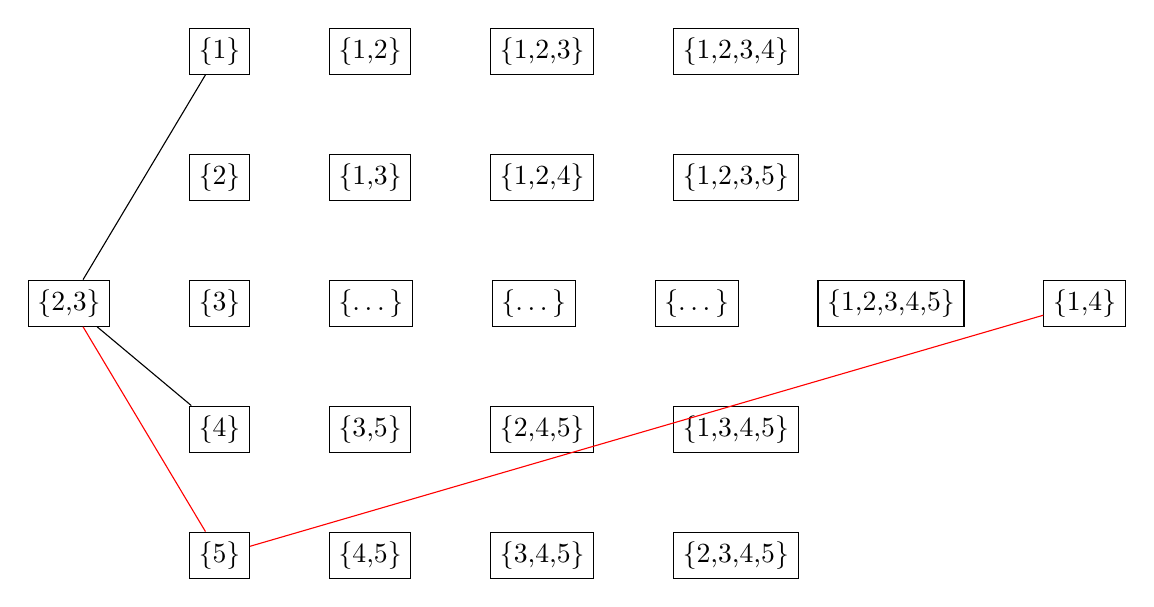
\begin{tikzpicture}[scale=1]
  \node (2) [draw, rectangle] {\{1\}};
  \node (3) [below=of 2, draw, rectangle] {\{2\}};
  \node (4) [below=of 3, draw, rectangle] {\{3\}};
  \node (5) [below=of 4, draw, rectangle] {\{4\}};
  \node (6) [below=of 5, draw, rectangle] {\{5\}};

  \node (1) [left=of 4, draw, rectangle] {\{2,3\}};

  \node (7) [right=of 2, draw, rectangle] {\{1,2\}};
  \node (8) [right=of 3, draw, rectangle] {\{1,3\}};
  \node (9) [right=of 4, draw, rectangle] {$\{\dots\}$};
  \node (10) [right=of 5, draw, rectangle] {\{3,5\}};
  \node (11) [right=of 6, draw, rectangle] {\{4,5\}};

  \node (12) [right=of 7, draw, rectangle] {\{1,2,3\}};
  \node (13) [right=of 8, draw, rectangle] {\{1,2,4\}};
  \node (14) [right=of 9, draw, rectangle] {$\{\dots\}$};
  \node (15) [right=of 10, draw, rectangle] {\{2,4,5\}};
  \node (16) [right=of 11, draw, rectangle] {\{3,4,5\}};

  \node (17) [right=of 12, draw, rectangle] {\{1,2,3,4\}};
  \node (18) [right=of 13, draw, rectangle] {\{1,2,3,5\}};
  \node (19) [right=of 14, draw, rectangle] {$\{\dots\}$};
  \node (20) [right=of 15, draw, rectangle] {\{1,3,4,5\}};
  \node (21) [right=of 16, draw, rectangle] {\{2,3,4,5\}};

  \node (22) [right=of 19, draw, rectangle] {\{1,2,3,4,5\}};

  \node (23) [right=of 22, draw, rectangle] {\{1,4\}};

  \draw[-, red]  (1) to node [auto] {} (6);
  \draw[-, red]  (6) to node [auto] {} (23);
  \draw[-]  (1) to node [auto] {} (2);
  \draw[-]  (1) to node [auto] {} (5);

\end{tikzpicture}
\end{scaletikzpicturetowidth}
\end{center}
\caption{Basic example of $3-$move Subset Sum Reconfiguration where $S = \{1,2,3,4,5\}$ and $A_1 = \{2,3\}$ and $A_2 = \{1,4\}$ and $x = 5$}\label{fig:3_move_subsetsum}
\end{figure}
\end{example}


%\chapter{Constrained Hypercube Path}
\label{chap:hypercube}

The $n$-hypercube is the graph with vertex set $\{0, 1\}^n$ such that two vertices are adjacent whenever their coordinates differ by exactly one component. In this section, we consider the following abstraction of reconfiguration problems involving subsets.

\begin{defn}{(Constrained Hypercube Path).} Given two vertices $s, t$ of the $n-$ hypercube, both contained in a polytope $P := \{x \in \mathbb{R}^n : Ax \leq b\}$ for some $A = (a_{ij}) \in \mathbb{Z}^{d \times n}$ and $b \in \mathbb{Z}^d$, does there exist a path from $s$ to $t$
in the hypercube, all vertices of which lie in $P$?
\end{defn}

\section{Problems correlation}
\todo{To find a better name for that chapter}
The knapsack (decision) problem involves exactly two linear constraints, and the Knapsack reconfiguration problem can be cast as a special case of the constrained hypercube path problem where $d = 2$. The definitions
are as follows.

\begin{defn}{(Knapsack (decision) Problem).} Given integers $l$ and $u$ and two sets of integers $S = \{a_1, a_2,\dots, a_n\}$ and $W = \{w_1, w_2,\dots, w_n\}$, does there exist a subset $A \subseteq [ n ]$ such that
\end{defn}

\begin{defn}{(Knapsack Reconfiguration Problem).} Given two solutions $A_1$ and $A_2$ to an instance of the knapsack problem, can $A_2$ be obtained by repeated $1-$move reconfiguration, begining with $A_i$, so that all intermediate subsets are also solutions ?
\end{defn}

\begin{theorem}{}The Constrained Hypercube Path problem is \PSPACE-complete, even when $d = O(1)$.
\end{theorem}

\begin{proof}{Many-way reconfiguration problem $\leq_p$ Constrained Hypercube Path problem}
The reduction is from the exact cover many-way reconfiguration problem, and is a modification of the
reduction given in the proof of Theorem $3.3$.  \todo{For this I have to understand and detail Theorem $3.3$}
\end{proof}


\section{Summary}
\begin{figure}[h!]
\begin{center}
\begin{scaletikzpicturetowidth}{\textwidth}
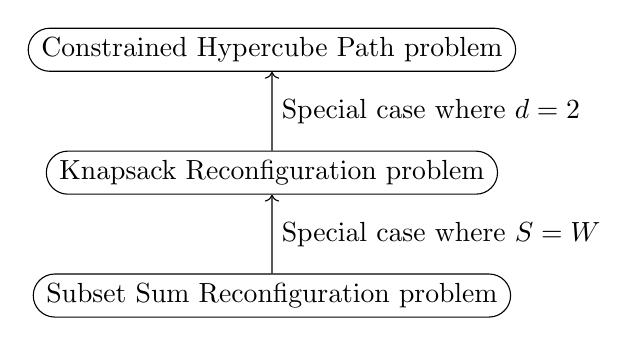
\begin{tikzpicture}[scale=1]
  \node (1) [draw, rounded rectangle] {Constrained Hypercube Path problem};
  \node (2) [below=of 1, draw, rounded rectangle] {Knapsack Reconfiguration problem};
  \node (3) [below=of 2, draw, rounded rectangle] {Subset Sum Reconfiguration problem};
  \draw[<-]  (1) to node [auto] {Special case where $d = 2$} (2);
  \draw[<-]  (2) to node [auto] {Special case where $S = W$} (3);
\end{tikzpicture}
\end{scaletikzpicturetowidth}
\end{center}
\caption{To define}\label{fig:specialCase}
\end{figure}

    \chapter{Conclusions and Future Works} \label{chap:conclu}
Throughout this thesis, we have researched and analysed reconfiguration problems by starting with the Nondeterministic Constraint Logic
which seems to be the go-to reduction in order to prove $\PSPACE$-hardness results. More specifically, we focused on the alternative
formulation of NCL and detailed the $\PSPACE$-completeness result of the sliding token problem. We then showed that the labelled variant of the
SLIDING TOKEN problem is also $\PSPACE$-complete. This latter result was then used to establish the complexity result of the Exact Cover merge
and split reconfiguration problem which was then used to prove the hardness of the $k$-move Subset sum reconfiguration problem for $k = 3$.
As a contribution to this part, we provided detailed explanatory examples and clarifications to complement the proof.
Every reconfiguration problems we encountered during our journey to the completion of this thesis is summed in fig \ref{fig:conclusion}.

\begin{figure}[H]
    \begin{center}
        \begin{scaletikzpicturetowidth}{\textwidth}
            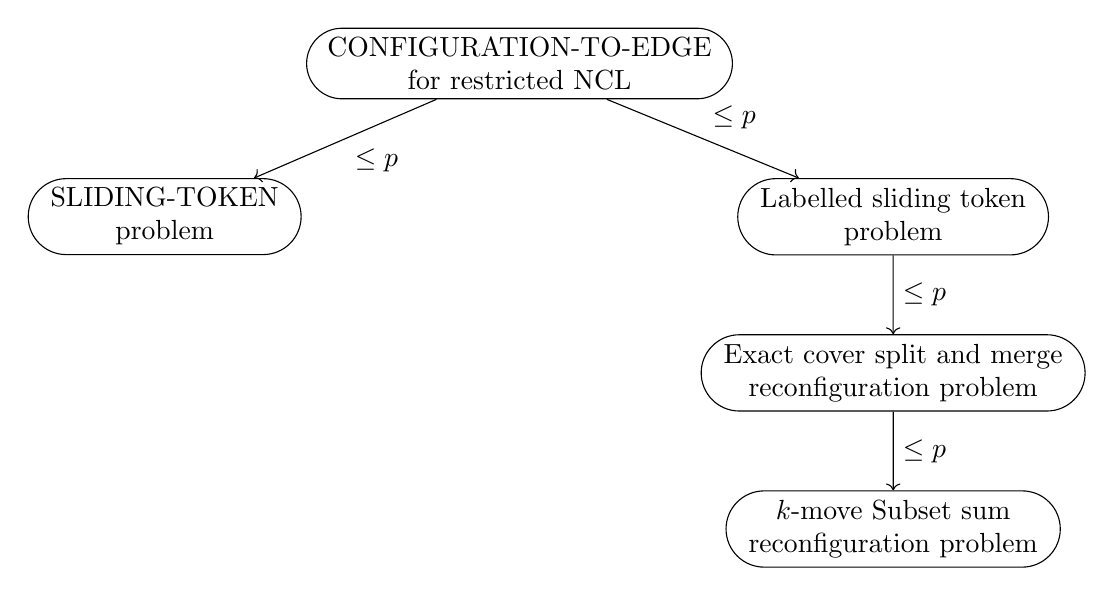
\begin{tikzpicture}[scale=0.8]
                \node (1) at (0,0) [draw, rounded rectangle, align=center] {CONFIGURATION-TO-EDGE\\for restricted NCL};
                \node (2)  [below left=of 1, draw, rounded rectangle, align=center] {SLIDING-TOKEN\\problem};
                \node (3)  [below right=of 1, draw, rounded rectangle, align=center] {Labelled sliding token\\problem};
                \node (4) [below=of 3, draw, rounded rectangle, align=center] {Exact cover split and merge\\ reconfiguration problem};
                \node (5) [below=of 4, draw, rounded rectangle, align=center] {$k$-move Subset sum\\reconfiguration problem};

                \draw[->]  (1) to node [auto] {$\leq{p}$} (2);
                \draw[->]  (1) to node [auto] {$\leq{p}$} (3);
                \draw[->]  (3) to node [auto] {$\leq{p}$} (4);
                \draw[->]  (4) to node [auto] {$\leq{p}$} (5);
            \end{tikzpicture}
        \end{scaletikzpicturetowidth}
    \end{center}
    \caption{$\PSPACE$-complete problems encountered and their relationship.}\label{fig:conclusion}
\end{figure}

%------------------------************************* Future works **********************------------------------

\section{Future works}

\subsection{SLIDING TOKENS problem}
Given a SLIDING TOKENS instance and two configurations $C_1$ and $C_2$, there may be several reconfiguration sequences to transform the given
initial configuration $C_1$ into $C_2$ (see figures \ref{fig:sequence1} and \ref{fig:sequence2}). Thus, the question of finding the
Shortest reconfiguration path in the SLIDING TOKENS problem naturally arised.


%-------------------------------------------- shortest 1 --------------------------------------------
\begin{figure}[H]
    \centering
    \begin{subfigure}[b]{0.4\textwidth}
        \begin{scaletikzpicturetowidth}{\textwidth}
            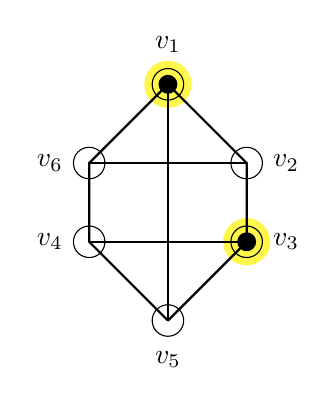
\begin{tikzpicture}[scale=1]
                \def\ver{0.12} %size of a vertex
                \def\xa{1}
                \def\ya{5}
                % highlight change
                \draw[fill=yellow, opacity=.7, draw=none] (\xa,\ya+3)  circle (0.3cm); % v1 ;
                \draw[fill=yellow, opacity=.7, draw=none] (\xa+1,\ya+1)  circle (0.3cm); % v3 ;

                %nodes
                \draw (\xa,\ya) circle (0.2cm);       % v5
                \draw (\xa+1,\ya+1) circle (0.2cm);   % v3
                \draw (\xa+1,\ya+2) circle (0.2cm);   % v2
                \draw (\xa,\ya+3) circle (0.2cm);     % v1
                \draw (\xa-1,\ya+2) circle (0.2cm);   % v6
                \draw (\xa-1,\ya+1) circle (0.2cm);   % v4

                %labels
                \node (1) at (\xa,\ya+3.5) {$v_1$};     % v1
                \node (2) at (\xa+1.5,\ya+2) {$v_2$};   % v2
                \node (3) at (\xa+1.5,\ya+1) {$v_3$};   % v3
                \node (5) at (\xa,\ya-0.5) {$v_5$};     % v5
                \node (4) at (\xa-1.5,\ya+1) {$v_4$};   % v4
                \node (6) at (\xa-1.5,\ya+2) {$v_6$};   % v6

                %token
                \path[fill] (\xa,\ya+3) circle (\ver);   % v1
                \path[fill] (\xa+1,\ya+1) circle (\ver);   % v3

                %edges
                \draw[thick] (\xa,\ya)--(\xa+1,\ya+1)--(\xa+1,\ya+2)--(\xa,\ya+3)--(\xa-1,\ya+2)--(\xa-1,\ya+1)--(\xa,\ya) ; % contour
                \draw[thick] (\xa,\ya)--(\xa,\ya+3) ;       % v5 - v1
                \draw[thick] (\xa+1,\ya+1)--(\xa-1,\ya+1) ; % v3 - v4
                \draw[thick] (\xa+1,\ya+2)--(\xa-1,\ya+2) ; % v2 - v6
            \end{tikzpicture}
        \end{scaletikzpicturetowidth}
        \caption{Initial Independent Set $I_1 = \{v_1, v_3\}$}
        \label{fig:s11}
    \end{subfigure}
    \begin{subfigure}[b]{0.4\textwidth}
        \begin{scaletikzpicturetowidth}{\textwidth}
            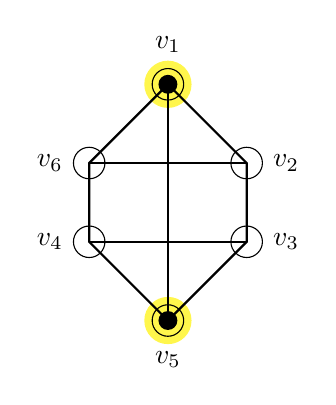
\begin{tikzpicture}[scale=1]
                \def\ver{0.12} %size of a vertex
                \def\xa{1}
                \def\ya{5}
                % highlight change
                \draw[fill=yellow, opacity=.7, draw=none] (\xa,\ya+3)  circle (0.3cm); % v1 ;
                \draw[fill=yellow, opacity=.7, draw=none] (\xa,\ya)  circle (0.3cm); % v5 ;

                %nodes
                \draw (\xa,\ya) circle (0.2cm);       % v5
                \draw (\xa+1,\ya+1) circle (0.2cm);   % v3
                \draw (\xa+1,\ya+2) circle (0.2cm);   % v2
                \draw (\xa,\ya+3) circle (0.2cm);     % v1
                \draw (\xa-1,\ya+2) circle (0.2cm);   % v6
                \draw (\xa-1,\ya+1) circle (0.2cm);   % v4

                %labels
                \node (1) at (\xa,\ya+3.5) {$v_1$};     % v1
                \node (2) at (\xa+1.5,\ya+2) {$v_2$};   % v2
                \node (3) at (\xa+1.5,\ya+1) {$v_3$};   % v3
                \node (5) at (\xa,\ya-0.5) {$v_5$};     % v5
                \node (4) at (\xa-1.5,\ya+1) {$v_4$};   % v4
                \node (6) at (\xa-1.5,\ya+2) {$v_6$};   % v6

                %token
                \path[fill] (\xa,\ya+3) circle (\ver);   % v1
                \path[fill] (\xa,\ya) circle (\ver);     % v5

                %edges
                \draw[thick] (\xa,\ya)--(\xa+1,\ya+1)--(\xa+1,\ya+2)--(\xa,\ya+3)--(\xa-1,\ya+2)--(\xa-1,\ya+1)--(\xa,\ya) ; % contour
                \draw[thick] (\xa,\ya)--(\xa,\ya+3) ;       % v5 - v1
                \draw[thick] (\xa+1,\ya+1)--(\xa-1,\ya+1) ; % v3 - v4
                \draw[thick] (\xa+1,\ya+2)--(\xa-1,\ya+2) ; % v2 - v6
            \end{tikzpicture}
        \end{scaletikzpicturetowidth}
        \caption{Intermediate Independent Set}
        \label{fig:s12}
    \end{subfigure}
    \begin{subfigure}[b]{0.4\textwidth}
        \begin{scaletikzpicturetowidth}{\textwidth}
            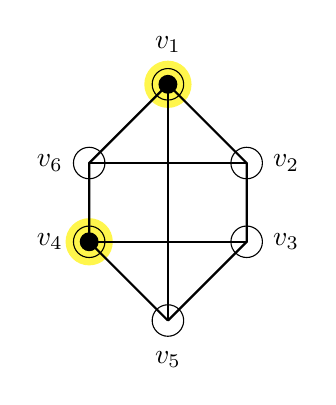
\begin{tikzpicture}[scale=1]
                \def\ver{0.12} %size of a vertex
                \def\xa{1}
                \def\ya{5}
                % highlight change
                \draw[fill=yellow, opacity=.7, draw=none] (\xa,\ya+3)  circle (0.3cm); % v1 ;
                \draw[fill=yellow, opacity=.7, draw=none] (\xa-1,\ya+1) circle (0.3cm); % v4 ;

                %nodes
                \draw (\xa,\ya) circle (0.2cm);       % v5
                \draw (\xa+1,\ya+1) circle (0.2cm);   % v3
                \draw (\xa+1,\ya+2) circle (0.2cm);   % v2
                \draw (\xa,\ya+3) circle (0.2cm);     % v1
                \draw (\xa-1,\ya+2) circle (0.2cm);   % v6
                \draw (\xa-1,\ya+1) circle (0.2cm);   % v4

                %labels
                \node (1) at (\xa,\ya+3.5) {$v_1$};     % v1
                \node (2) at (\xa+1.5,\ya+2) {$v_2$};   % v2
                \node (3) at (\xa+1.5,\ya+1) {$v_3$};   % v3
                \node (5) at (\xa,\ya-0.5) {$v_5$};     % v5
                \node (4) at (\xa-1.5,\ya+1) {$v_4$};   % v4
                \node (6) at (\xa-1.5,\ya+2) {$v_6$};   % v6

                %token
                \path[fill] (\xa,\ya+3) circle (\ver);   % v1
                \path[fill] (\xa-1,\ya+1) circle (\ver); % v4

                %edges
                \draw[thick] (\xa,\ya)--(\xa+1,\ya+1)--(\xa+1,\ya+2)--(\xa,\ya+3)--(\xa-1,\ya+2)--(\xa-1,\ya+1)--(\xa,\ya) ; % contour
                \draw[thick] (\xa,\ya)--(\xa,\ya+3) ;       % v5 - v1
                \draw[thick] (\xa+1,\ya+1)--(\xa-1,\ya+1) ; % v3 - v4
                \draw[thick] (\xa+1,\ya+2)--(\xa-1,\ya+2) ; % v2 - v6
            \end{tikzpicture}
        \end{scaletikzpicturetowidth}
        \caption{Target Independent Set $I_2 = \{v_2, v_4\}$}
        \label{fig:s13}
    \end{subfigure}
    \begin{subfigure}[b]{0.4\textwidth}
        \begin{scaletikzpicturetowidth}{\textwidth}
            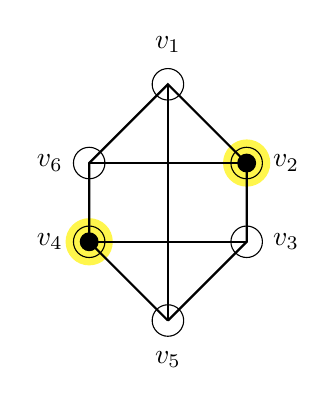
\begin{tikzpicture}[scale=1]
                \def\ver{0.12} %size of a vertex
                \def\xa{1}
                \def\ya{5}
                % highlight change
                \draw[fill=yellow, opacity=.7, draw=none] (\xa+1,\ya+2) circle (0.3cm); % v2 ;
                \draw[fill=yellow, opacity=.7, draw=none] (\xa-1,\ya+1) circle (0.3cm); % v4 ;

                %nodes
                \draw (\xa,\ya) circle (0.2cm);       % v5
                \draw (\xa+1,\ya+1) circle (0.2cm);   % v3
                \draw (\xa+1,\ya+2) circle (0.2cm);   % v2
                \draw (\xa,\ya+3) circle (0.2cm);     % v1
                \draw (\xa-1,\ya+2) circle (0.2cm);   % v6
                \draw (\xa-1,\ya+1) circle (0.2cm);   % v4

                %labels
                \node (1) at (\xa,\ya+3.5) {$v_1$};     % v1
                \node (2) at (\xa+1.5,\ya+2) {$v_2$};   % v2
                \node (3) at (\xa+1.5,\ya+1) {$v_3$};   % v3
                \node (5) at (\xa,\ya-0.5) {$v_5$};     % v5
                \node (4) at (\xa-1.5,\ya+1) {$v_4$};   % v4
                \node (6) at (\xa-1.5,\ya+2) {$v_6$};   % v6

                %token
                \path[fill] (\xa+1,\ya+2) circle (\ver); % v2
                \path[fill] (\xa-1,\ya+1) circle (\ver); % v4

                %edges
                \draw[thick] (\xa,\ya)--(\xa+1,\ya+1)--(\xa+1,\ya+2)--(\xa,\ya+3)--(\xa-1,\ya+2)--(\xa-1,\ya+1)--(\xa,\ya) ; % contour
                \draw[thick] (\xa,\ya)--(\xa,\ya+3) ;       % v5 - v1
                \draw[thick] (\xa+1,\ya+1)--(\xa-1,\ya+1) ; % v3 - v4
                \draw[thick] (\xa+1,\ya+2)--(\xa-1,\ya+2) ; % v2 - v6
            \end{tikzpicture}
        \end{scaletikzpicturetowidth}
        \caption{A $3$-regular graph $G=(V,E)$ and initial independent set $I_1 = \{v_1, v_3\}$}
        \label{fig:s14}
    \end{subfigure}
    \caption{Configuration-to-edge input instance}
    \label{fig:sequence1}
\end{figure}

%-------------------------------------------- shortest 2 --------------------------------------------
\begin{figure}[H]
    \centering
    \begin{subfigure}[b]{0.3\textwidth}
        \begin{scaletikzpicturetowidth}{\textwidth}
            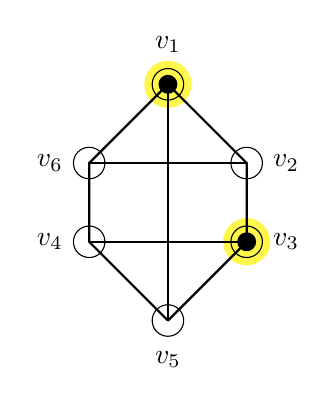
\begin{tikzpicture}[scale=1]
                \def\ver{0.12} %size of a vertex
                \def\xa{1}
                \def\ya{5}
                % highlight change
                \draw[fill=yellow, opacity=.7, draw=none] (\xa,\ya+3)  circle (0.3cm); % v1 ;
                \draw[fill=yellow, opacity=.7, draw=none] (\xa+1,\ya+1)  circle (0.3cm); % v3 ;

                %nodes
                \draw (\xa,\ya) circle (0.2cm);       % v5
                \draw (\xa+1,\ya+1) circle (0.2cm);   % v3
                \draw (\xa+1,\ya+2) circle (0.2cm);   % v2
                \draw (\xa,\ya+3) circle (0.2cm);     % v1
                \draw (\xa-1,\ya+2) circle (0.2cm);   % v6
                \draw (\xa-1,\ya+1) circle (0.2cm);   % v4

                %labels
                \node (1) at (\xa,\ya+3.5) {$v_1$};     % v1
                \node (2) at (\xa+1.5,\ya+2) {$v_2$};   % v2
                \node (3) at (\xa+1.5,\ya+1) {$v_3$};   % v3
                \node (5) at (\xa,\ya-0.5) {$v_5$};     % v5
                \node (4) at (\xa-1.5,\ya+1) {$v_4$};   % v4
                \node (6) at (\xa-1.5,\ya+2) {$v_6$};   % v6

                %token
                \path[fill] (\xa,\ya+3) circle (\ver);   % v1
                \path[fill] (\xa+1,\ya+1) circle (\ver);   % v3

                %edges
                \draw[thick] (\xa,\ya)--(\xa+1,\ya+1)--(\xa+1,\ya+2)--(\xa,\ya+3)--(\xa-1,\ya+2)--(\xa-1,\ya+1)--(\xa,\ya) ; % contour
                \draw[thick] (\xa,\ya)--(\xa,\ya+3) ;       % v5 - v1
                \draw[thick] (\xa+1,\ya+1)--(\xa-1,\ya+1) ; % v3 - v4
                \draw[thick] (\xa+1,\ya+2)--(\xa-1,\ya+2) ; % v2 - v6
            \end{tikzpicture}
        \end{scaletikzpicturetowidth}
        \caption{Initial Independent Set $I_1 = \{v_1, v_3\}$}
        \label{fig:s21}
    \end{subfigure}
    \begin{subfigure}[b]{0.3\textwidth}
        \begin{scaletikzpicturetowidth}{\textwidth}
            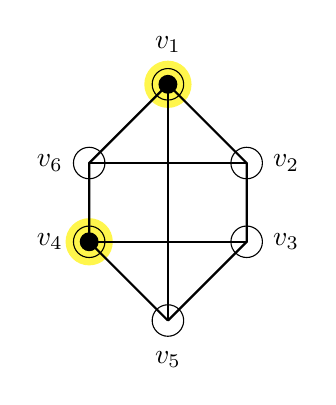
\begin{tikzpicture}[scale=1]
                \def\ver{0.12} %size of a vertex
                \def\xa{1}
                \def\ya{5}
                % highlight change
                \draw[fill=yellow, opacity=.7, draw=none] (\xa,\ya+3)  circle (0.3cm); % v1 ;
                \draw[fill=yellow, opacity=.7, draw=none] (\xa-1,\ya+1)  circle (0.3cm); % v4 ;

                %nodes
                \draw (\xa,\ya) circle (0.2cm);       % v5
                \draw (\xa+1,\ya+1) circle (0.2cm);   % v3
                \draw (\xa+1,\ya+2) circle (0.2cm);   % v2
                \draw (\xa,\ya+3) circle (0.2cm);     % v1
                \draw (\xa-1,\ya+2) circle (0.2cm);   % v6
                \draw (\xa-1,\ya+1) circle (0.2cm);   % v4

                %labels
                \node (1) at (\xa,\ya+3.5) {$v_1$};     % v1
                \node (2) at (\xa+1.5,\ya+2) {$v_2$};   % v2
                \node (3) at (\xa+1.5,\ya+1) {$v_3$};   % v3
                \node (5) at (\xa,\ya-0.5) {$v_5$};     % v5
                \node (4) at (\xa-1.5,\ya+1) {$v_4$};   % v4
                \node (6) at (\xa-1.5,\ya+2) {$v_6$};   % v6

                %token
                \path[fill] (\xa,\ya+3) circle (\ver);   % v1
                \path[fill] (\xa-1,\ya+1) circle (\ver); % v4

                %edges
                \draw[thick] (\xa,\ya)--(\xa+1,\ya+1)--(\xa+1,\ya+2)--(\xa,\ya+3)--(\xa-1,\ya+2)--(\xa-1,\ya+1)--(\xa,\ya) ; % contour
                \draw[thick] (\xa,\ya)--(\xa,\ya+3) ;       % v5 - v1
                \draw[thick] (\xa+1,\ya+1)--(\xa-1,\ya+1) ; % v3 - v4
                \draw[thick] (\xa+1,\ya+2)--(\xa-1,\ya+2) ; % v2 - v6
            \end{tikzpicture}
        \end{scaletikzpicturetowidth}
        \caption{Intermediate Independent Set}
        \label{fig:s22}
    \end{subfigure}
    \begin{subfigure}[b]{0.3\textwidth}
        \begin{scaletikzpicturetowidth}{\textwidth}
            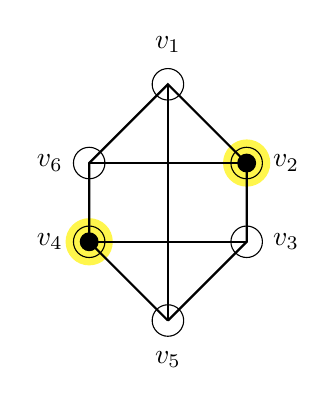
\begin{tikzpicture}[scale=1]
                \def\ver{0.12} %size of a vertex
                \def\xa{1}
                \def\ya{5}
                % highlight change
                \draw[fill=yellow, opacity=.7, draw=none] (\xa+1,\ya+2)  circle (0.3cm); % v2 ;
                \draw[fill=yellow, opacity=.7, draw=none] (\xa-1,\ya+1) circle (0.3cm); % v4 ;

                %nodes
                \draw (\xa,\ya) circle (0.2cm);       % v5
                \draw (\xa+1,\ya+1) circle (0.2cm);   % v3
                \draw (\xa+1,\ya+2) circle (0.2cm);   % v2
                \draw (\xa,\ya+3) circle (0.2cm);     % v1
                \draw (\xa-1,\ya+2) circle (0.2cm);   % v6
                \draw (\xa-1,\ya+1) circle (0.2cm);   % v4

                %labels
                \node (1) at (\xa,\ya+3.5) {$v_1$};     % v1
                \node (2) at (\xa+1.5,\ya+2) {$v_2$};   % v2
                \node (3) at (\xa+1.5,\ya+1) {$v_3$};   % v3
                \node (5) at (\xa,\ya-0.5) {$v_5$};     % v5
                \node (4) at (\xa-1.5,\ya+1) {$v_4$};   % v4
                \node (6) at (\xa-1.5,\ya+2) {$v_6$};   % v6

                %token
                \path[fill] (\xa+1,\ya+2) circle (\ver);   % v2
                \path[fill] (\xa-1,\ya+1) circle (\ver); % v4

                %edges
                \draw[thick] (\xa,\ya)--(\xa+1,\ya+1)--(\xa+1,\ya+2)--(\xa,\ya+3)--(\xa-1,\ya+2)--(\xa-1,\ya+1)--(\xa,\ya) ; % contour
                \draw[thick] (\xa,\ya)--(\xa,\ya+3) ;       % v5 - v1
                \draw[thick] (\xa+1,\ya+1)--(\xa-1,\ya+1) ; % v3 - v4
                \draw[thick] (\xa+1,\ya+2)--(\xa-1,\ya+2) ; % v2 - v6
            \end{tikzpicture}
        \end{scaletikzpicturetowidth}
        \caption{Target Independent Set $I_2 = \{v_2, v_4\}$}
        \label{fig:s23}
    \end{subfigure}
    \caption{Configuration-to-edge input instance}
    \label{fig:sequence2}
\end{figure}

However this question has already been asked by Yamada and Uehara in 2016, defined below and remains open. The difficulty lies in
computing the reconfiguration graph.
\begin{flushleft}
    Shortest Sliding Token [Yamada and Uehara 2016]\\
    \textbf{Instance: } A yes-instance $(G, I, J)$ of Sliding Token, where $I, J$ are independent sets of a graph $G$. \\
    \textbf{Question: } Find a shortest TS-sequence that transforms $I$ into $J$ (and vice versa) \\
\end{flushleft}

On the bright side, in the past years positive results have been established for cographs, interval graphs, caterpillars, trees,
prefect graphs and spider graphs. Those interesting results are summed up below.
\begin{theorem}(Kaminski et al. 2012)
It is $\NP$-complete to decide if there is a TS-sequence having at most $l$ token-slides between two independent sets $I, J$ of a
perfect graph $G$ even when $l$ is polynomial in $|V(G)|$.
\end{theorem}

\begin{theorem}(Kaminski et al. 2012)
Shortest Sliding Token can be solved in linear time for cographs (P4-free graphs).
\end{theorem}

\begin{theorem}(Yamada and Uehara 2016)
Shortest Sliding Token can be solved in polynomial time for proper interval graphs, trivially perfect graphs, and caterpillars.
\end{theorem}

\begin{theorem}(Sugimori, AAAC 2018)
Shortest Sliding Token can be solved in $O(poly(n))$ time when the input graph is a tree on $n$ vertices.
\end{theorem}

\begin{theorem}(Ryuhei Uehara, CIAC 2019)
Shortest Sliding Token can be solved in $O(n^2)$ time when the input graph is a spider (i.e., a tree having exactly one
vertex of degree at least $3$) on $n$ vertices.
\end{theorem}


\subsection{$3$-move SUBSET SUM RECONFIGURATION problem}
Recall that we studied the following problem in chapter \ref{chap:subset-sum-reconf} :
\begin{defn}{($k$-move SUBSET SUM RECONFIGURATION Problem).} Given two solutions $A_1$ and $A_2$ to an instance of the subset sum problem,
can $A_2$ be obtained by repeated $k$-move reconfiguration, beginning with $A_1$, so that all intermediate subsets are also solutions?
\end{defn}

It would be interesting to study the connectivity question of the $k$-move SUBSET SUM RECONFIGURATION problem defined below :
\begin{defn}{($k$-move SUBSET SUM RECONFIGURATION Problem conn).} Given an integer $x$ and a set of integers $S = \{a_1, a_2, \dots, a_n\}$,
let $G(S)$ be the subgraph graph induced by the feasible solutions of $S$ where there is an edge between two vertices
of $G(S)$ iff the symmetric difference is at most $k$. Is $G(S)$ connected ?
\end{defn}

Another question concerns finding an optimal coloring with $k$ colors that is smaller than $23$ for the ECR problem.

\chapter{Future works}

While working on this thesis a few questions popped up in my brain :

\paragraph{Shortest reconfiguration path in the sliding token reconfiguration problem.}

%-------------------------------------------- Init --------------------------------------------
\begin{figure}[H]
    \centering
    \begin{subfigure}[b]{0.4\textwidth}
        \begin{scaletikzpicturetowidth}{\textwidth}
            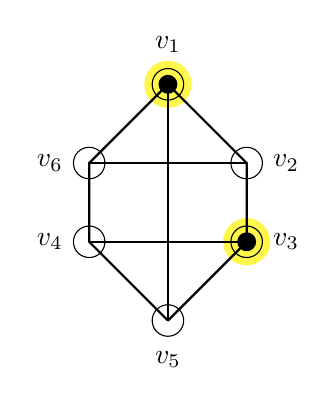
\begin{tikzpicture}[scale=1]
                \def\ver{0.12} %size of a vertex
                \def\xa{1}
                \def\ya{5}
                % highlight change
                \draw[fill=yellow, opacity=.7, draw=none] (\xa,\ya+3)  circle (0.3cm); % v1 ;
                \draw[fill=yellow, opacity=.7, draw=none] (\xa+1,\ya+1)  circle (0.3cm); % v3 ;

                %nodes
                \draw (\xa,\ya) circle (0.2cm);       % v5
                \draw (\xa+1,\ya+1) circle (0.2cm);   % v3
                \draw (\xa+1,\ya+2) circle (0.2cm);   % v2
                \draw (\xa,\ya+3) circle (0.2cm);     % v1
                \draw (\xa-1,\ya+2) circle (0.2cm);   % v6
                \draw (\xa-1,\ya+1) circle (0.2cm);   % v4

                %labels
                \node (1) at (\xa,\ya+3.5) {$v_1$};     % v1
                \node (2) at (\xa+1.5,\ya+2) {$v_2$};   % v2
                \node (3) at (\xa+1.5,\ya+1) {$v_3$};   % v3
                \node (5) at (\xa,\ya-0.5) {$v_5$};     % v5
                \node (4) at (\xa-1.5,\ya+1) {$v_4$};   % v4
                \node (6) at (\xa-1.5,\ya+2) {$v_6$};   % v6

                %token
                \path[fill] (\xa,\ya+3) circle (\ver);   % v1
                \path[fill] (\xa+1,\ya+1) circle (\ver);   % v3

                %edges
                \draw[thick] (\xa,\ya)--(\xa+1,\ya+1)--(\xa+1,\ya+2)--(\xa,\ya+3)--(\xa-1,\ya+2)--(\xa-1,\ya+1)--(\xa,\ya) ; % contour
                \draw[thick] (\xa,\ya)--(\xa,\ya+3) ;       % v5 - v1
                \draw[thick] (\xa+1,\ya+1)--(\xa-1,\ya+1) ; % v3 - v4
                \draw[thick] (\xa+1,\ya+2)--(\xa-1,\ya+2) ; % v2 - v6
            \end{tikzpicture}
        \end{scaletikzpicturetowidth}
        \caption{A $3$-regular graph $G=(V,E)$ and initial independent set $I_1 = \{v_1, v_3\}$}
        \label{fig:s1}
    \end{subfigure}
    \begin{subfigure}[b]{0.4\textwidth}
        \begin{scaletikzpicturetowidth}{\textwidth}
            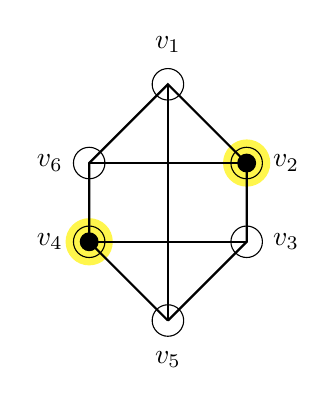
\begin{tikzpicture}[scale=1]
                \def\ver{0.12} %size of a vertex
                \def\xa{1}
                \def\ya{5}
                % highlight change
                \draw[fill=yellow, opacity=.7, draw=none] (\xa+1,\ya+2)  circle (0.3cm); % v2 ;
                \draw[fill=yellow, opacity=.7, draw=none] (\xa-1,\ya+1)  circle (0.3cm); % v4 ;

                %nodes
                \draw (\xa,\ya) circle (0.2cm);       % v5
                \draw (\xa+1,\ya+1) circle (0.2cm);   % v3
                \draw (\xa+1,\ya+2) circle (0.2cm);   % v2
                \draw (\xa,\ya+3) circle (0.2cm);     % v1
                \draw (\xa-1,\ya+2) circle (0.2cm);   % v6
                \draw (\xa-1,\ya+1) circle (0.2cm);   % v4

                %labels
                \node (1) at (\xa,\ya+3.5) {$v_1$};     % v1
                \node (2) at (\xa+1.5,\ya+2) {$v_2$};   % v2
                \node (3) at (\xa+1.5,\ya+1) {$v_3$};   % v3
                \node (5) at (\xa,\ya-0.5) {$v_5$};     % v5
                \node (4) at (\xa-1.5,\ya+1) {$v_4$};   % v4
                \node (6) at (\xa-1.5,\ya+2) {$v_6$};   % v6

                %token
                \path[fill] (\xa+1,\ya+2) circle (\ver);   % v2
                \path[fill] (\xa-1,\ya+1) circle (\ver);   % v4

                %edges
                \draw[thick] (\xa,\ya)--(\xa+1,\ya+1)--(\xa+1,\ya+2)--(\xa,\ya+3)--(\xa-1,\ya+2)--(\xa-1,\ya+1)--(\xa,\ya) ; % contour
                \draw[thick] (\xa,\ya)--(\xa,\ya+3) ;       % v5 - v1
                \draw[thick] (\xa+1,\ya+1)--(\xa-1,\ya+1) ; % v3 - v4
                \draw[thick] (\xa+1,\ya+2)--(\xa-1,\ya+2) ; % v2 - v6
            \end{tikzpicture}
        \end{scaletikzpicturetowidth}
        \caption{A $3$-regular graph $G=(V,E)$ and initial independent set $I_1 = \{v_1, v_3\}$}
        \label{fig:s2}
    \end{subfigure}
    \caption{Configuration-to-edge input instance}
    \label{fig:s1}
\end{figure}

%-------------------------------------------- shortest 1 --------------------------------------------
\begin{figure}[H]
    \centering
    \begin{subfigure}[b]{0.4\textwidth}
        \begin{scaletikzpicturetowidth}{\textwidth}
            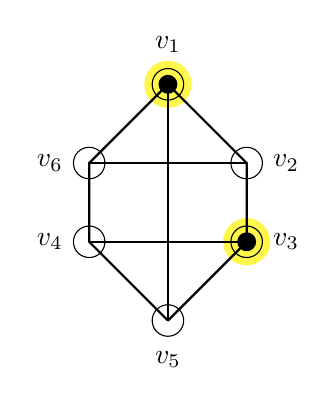
\begin{tikzpicture}[scale=1]
                \def\ver{0.12} %size of a vertex
                \def\xa{1}
                \def\ya{5}
                % highlight change
                \draw[fill=yellow, opacity=.7, draw=none] (\xa,\ya+3)  circle (0.3cm); % v1 ;
                \draw[fill=yellow, opacity=.7, draw=none] (\xa+1,\ya+1)  circle (0.3cm); % v3 ;

                %nodes
                \draw (\xa,\ya) circle (0.2cm);       % v5
                \draw (\xa+1,\ya+1) circle (0.2cm);   % v3
                \draw (\xa+1,\ya+2) circle (0.2cm);   % v2
                \draw (\xa,\ya+3) circle (0.2cm);     % v1
                \draw (\xa-1,\ya+2) circle (0.2cm);   % v6
                \draw (\xa-1,\ya+1) circle (0.2cm);   % v4

                %labels
                \node (1) at (\xa,\ya+3.5) {$v_1$};     % v1
                \node (2) at (\xa+1.5,\ya+2) {$v_2$};   % v2
                \node (3) at (\xa+1.5,\ya+1) {$v_3$};   % v3
                \node (5) at (\xa,\ya-0.5) {$v_5$};     % v5
                \node (4) at (\xa-1.5,\ya+1) {$v_4$};   % v4
                \node (6) at (\xa-1.5,\ya+2) {$v_6$};   % v6

                %token
                \path[fill] (\xa,\ya+3) circle (\ver);   % v1
                \path[fill] (\xa+1,\ya+1) circle (\ver);   % v3

                %edges
                \draw[thick] (\xa,\ya)--(\xa+1,\ya+1)--(\xa+1,\ya+2)--(\xa,\ya+3)--(\xa-1,\ya+2)--(\xa-1,\ya+1)--(\xa,\ya) ; % contour
                \draw[thick] (\xa,\ya)--(\xa,\ya+3) ;       % v5 - v1
                \draw[thick] (\xa+1,\ya+1)--(\xa-1,\ya+1) ; % v3 - v4
                \draw[thick] (\xa+1,\ya+2)--(\xa-1,\ya+2) ; % v2 - v6
            \end{tikzpicture}
        \end{scaletikzpicturetowidth}
        \caption{A $3$-regular graph $G=(V,E)$ and initial independent set $I_1 = \{v_1, v_3\}$}
        \label{fig:s11}
    \end{subfigure}
    \begin{subfigure}[b]{0.4\textwidth}
        \begin{scaletikzpicturetowidth}{\textwidth}
            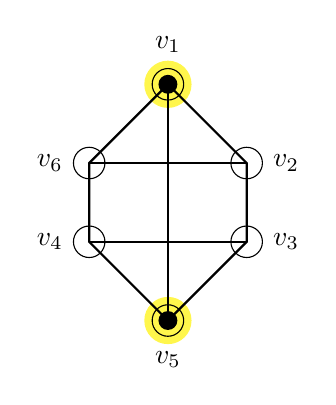
\begin{tikzpicture}[scale=1]
                \def\ver{0.12} %size of a vertex
                \def\xa{1}
                \def\ya{5}
                % highlight change
                \draw[fill=yellow, opacity=.7, draw=none] (\xa,\ya+3)  circle (0.3cm); % v1 ;
                \draw[fill=yellow, opacity=.7, draw=none] (\xa,\ya)  circle (0.3cm); % v5 ;

                %nodes
                \draw (\xa,\ya) circle (0.2cm);       % v5
                \draw (\xa+1,\ya+1) circle (0.2cm);   % v3
                \draw (\xa+1,\ya+2) circle (0.2cm);   % v2
                \draw (\xa,\ya+3) circle (0.2cm);     % v1
                \draw (\xa-1,\ya+2) circle (0.2cm);   % v6
                \draw (\xa-1,\ya+1) circle (0.2cm);   % v4

                %labels
                \node (1) at (\xa,\ya+3.5) {$v_1$};     % v1
                \node (2) at (\xa+1.5,\ya+2) {$v_2$};   % v2
                \node (3) at (\xa+1.5,\ya+1) {$v_3$};   % v3
                \node (5) at (\xa,\ya-0.5) {$v_5$};     % v5
                \node (4) at (\xa-1.5,\ya+1) {$v_4$};   % v4
                \node (6) at (\xa-1.5,\ya+2) {$v_6$};   % v6

                %token
                \path[fill] (\xa,\ya+3) circle (\ver);   % v1
                \path[fill] (\xa,\ya) circle (\ver);     % v5

                %edges
                \draw[thick] (\xa,\ya)--(\xa+1,\ya+1)--(\xa+1,\ya+2)--(\xa,\ya+3)--(\xa-1,\ya+2)--(\xa-1,\ya+1)--(\xa,\ya) ; % contour
                \draw[thick] (\xa,\ya)--(\xa,\ya+3) ;       % v5 - v1
                \draw[thick] (\xa+1,\ya+1)--(\xa-1,\ya+1) ; % v3 - v4
                \draw[thick] (\xa+1,\ya+2)--(\xa-1,\ya+2) ; % v2 - v6
            \end{tikzpicture}
        \end{scaletikzpicturetowidth}
        \caption{A $3$-regular graph $G=(V,E)$ and initial independent set $I_1 = \{v_1, v_3\}$}
        \label{fig:s12}
    \end{subfigure}
    \begin{subfigure}[b]{0.4\textwidth}
        \begin{scaletikzpicturetowidth}{\textwidth}
            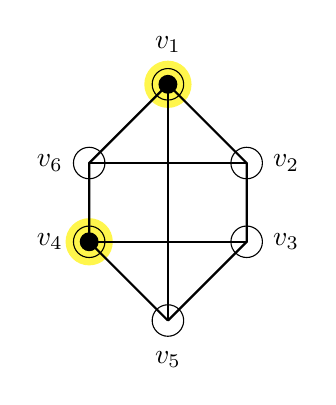
\begin{tikzpicture}[scale=1]
                \def\ver{0.12} %size of a vertex
                \def\xa{1}
                \def\ya{5}
                % highlight change
                \draw[fill=yellow, opacity=.7, draw=none] (\xa,\ya+3)  circle (0.3cm); % v1 ;
                \draw[fill=yellow, opacity=.7, draw=none] (\xa-1,\ya+1) circle (0.3cm); % v4 ;

                %nodes
                \draw (\xa,\ya) circle (0.2cm);       % v5
                \draw (\xa+1,\ya+1) circle (0.2cm);   % v3
                \draw (\xa+1,\ya+2) circle (0.2cm);   % v2
                \draw (\xa,\ya+3) circle (0.2cm);     % v1
                \draw (\xa-1,\ya+2) circle (0.2cm);   % v6
                \draw (\xa-1,\ya+1) circle (0.2cm);   % v4

                %labels
                \node (1) at (\xa,\ya+3.5) {$v_1$};     % v1
                \node (2) at (\xa+1.5,\ya+2) {$v_2$};   % v2
                \node (3) at (\xa+1.5,\ya+1) {$v_3$};   % v3
                \node (5) at (\xa,\ya-0.5) {$v_5$};     % v5
                \node (4) at (\xa-1.5,\ya+1) {$v_4$};   % v4
                \node (6) at (\xa-1.5,\ya+2) {$v_6$};   % v6

                %token
                \path[fill] (\xa,\ya+3) circle (\ver);   % v1
                \path[fill] (\xa-1,\ya+1) circle (\ver); % v4

                %edges
                \draw[thick] (\xa,\ya)--(\xa+1,\ya+1)--(\xa+1,\ya+2)--(\xa,\ya+3)--(\xa-1,\ya+2)--(\xa-1,\ya+1)--(\xa,\ya) ; % contour
                \draw[thick] (\xa,\ya)--(\xa,\ya+3) ;       % v5 - v1
                \draw[thick] (\xa+1,\ya+1)--(\xa-1,\ya+1) ; % v3 - v4
                \draw[thick] (\xa+1,\ya+2)--(\xa-1,\ya+2) ; % v2 - v6
            \end{tikzpicture}
        \end{scaletikzpicturetowidth}
        \caption{A $3$-regular graph $G=(V,E)$ and initial independent set $I_1 = \{v_1, v_3\}$}
        \label{fig:s13}
    \end{subfigure}
    \begin{subfigure}[b]{0.4\textwidth}
        \begin{scaletikzpicturetowidth}{\textwidth}
            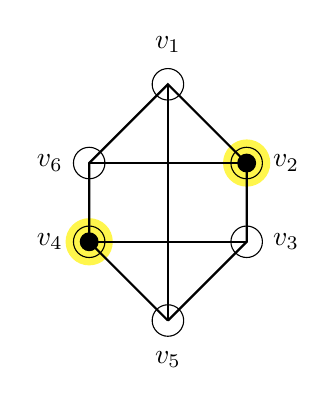
\begin{tikzpicture}[scale=1]
                \def\ver{0.12} %size of a vertex
                \def\xa{1}
                \def\ya{5}
                % highlight change
                \draw[fill=yellow, opacity=.7, draw=none] (\xa+1,\ya+2) circle (0.3cm); % v2 ;
                \draw[fill=yellow, opacity=.7, draw=none] (\xa-1,\ya+1) circle (0.3cm); % v4 ;

                %nodes
                \draw (\xa,\ya) circle (0.2cm);       % v5
                \draw (\xa+1,\ya+1) circle (0.2cm);   % v3
                \draw (\xa+1,\ya+2) circle (0.2cm);   % v2
                \draw (\xa,\ya+3) circle (0.2cm);     % v1
                \draw (\xa-1,\ya+2) circle (0.2cm);   % v6
                \draw (\xa-1,\ya+1) circle (0.2cm);   % v4

                %labels
                \node (1) at (\xa,\ya+3.5) {$v_1$};     % v1
                \node (2) at (\xa+1.5,\ya+2) {$v_2$};   % v2
                \node (3) at (\xa+1.5,\ya+1) {$v_3$};   % v3
                \node (5) at (\xa,\ya-0.5) {$v_5$};     % v5
                \node (4) at (\xa-1.5,\ya+1) {$v_4$};   % v4
                \node (6) at (\xa-1.5,\ya+2) {$v_6$};   % v6

                %token
                \path[fill] (\xa+1,\ya+2) circle (\ver); % v2
                \path[fill] (\xa-1,\ya+1) circle (\ver); % v4

                %edges
                \draw[thick] (\xa,\ya)--(\xa+1,\ya+1)--(\xa+1,\ya+2)--(\xa,\ya+3)--(\xa-1,\ya+2)--(\xa-1,\ya+1)--(\xa,\ya) ; % contour
                \draw[thick] (\xa,\ya)--(\xa,\ya+3) ;       % v5 - v1
                \draw[thick] (\xa+1,\ya+1)--(\xa-1,\ya+1) ; % v3 - v4
                \draw[thick] (\xa+1,\ya+2)--(\xa-1,\ya+2) ; % v2 - v6
            \end{tikzpicture}
        \end{scaletikzpicturetowidth}
        \caption{A $3$-regular graph $G=(V,E)$ and initial independent set $I_1 = \{v_1, v_3\}$}
        \label{fig:s13}
    \end{subfigure}
    \caption{Configuration-to-edge input instance}
    \label{fig:s2}
\end{figure}

%-------------------------------------------- shortest 2 --------------------------------------------
\begin{figure}[H]
    \centering
    \begin{subfigure}[b]{0.4\textwidth}
        \begin{scaletikzpicturetowidth}{\textwidth}
            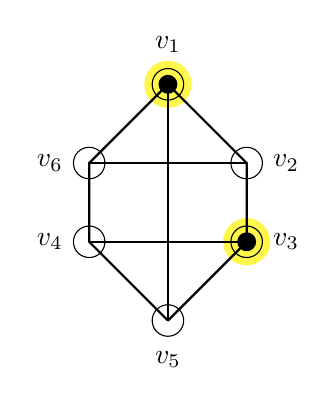
\begin{tikzpicture}[scale=1]
                \def\ver{0.12} %size of a vertex
                \def\xa{1}
                \def\ya{5}
                % highlight change
                \draw[fill=yellow, opacity=.7, draw=none] (\xa,\ya+3)  circle (0.3cm); % v1 ;
                \draw[fill=yellow, opacity=.7, draw=none] (\xa+1,\ya+1)  circle (0.3cm); % v3 ;

                %nodes
                \draw (\xa,\ya) circle (0.2cm);       % v5
                \draw (\xa+1,\ya+1) circle (0.2cm);   % v3
                \draw (\xa+1,\ya+2) circle (0.2cm);   % v2
                \draw (\xa,\ya+3) circle (0.2cm);     % v1
                \draw (\xa-1,\ya+2) circle (0.2cm);   % v6
                \draw (\xa-1,\ya+1) circle (0.2cm);   % v4

                %labels
                \node (1) at (\xa,\ya+3.5) {$v_1$};     % v1
                \node (2) at (\xa+1.5,\ya+2) {$v_2$};   % v2
                \node (3) at (\xa+1.5,\ya+1) {$v_3$};   % v3
                \node (5) at (\xa,\ya-0.5) {$v_5$};     % v5
                \node (4) at (\xa-1.5,\ya+1) {$v_4$};   % v4
                \node (6) at (\xa-1.5,\ya+2) {$v_6$};   % v6

                %token
                \path[fill] (\xa,\ya+3) circle (\ver);   % v1
                \path[fill] (\xa+1,\ya+1) circle (\ver);   % v3

                %edges
                \draw[thick] (\xa,\ya)--(\xa+1,\ya+1)--(\xa+1,\ya+2)--(\xa,\ya+3)--(\xa-1,\ya+2)--(\xa-1,\ya+1)--(\xa,\ya) ; % contour
                \draw[thick] (\xa,\ya)--(\xa,\ya+3) ;       % v5 - v1
                \draw[thick] (\xa+1,\ya+1)--(\xa-1,\ya+1) ; % v3 - v4
                \draw[thick] (\xa+1,\ya+2)--(\xa-1,\ya+2) ; % v2 - v6
            \end{tikzpicture}
        \end{scaletikzpicturetowidth}
        \caption{A $3$-regular graph $G=(V,E)$ and initial independent set $I_1 = \{v_1, v_3\}$}
        \label{fig:s11}
    \end{subfigure}
    \begin{subfigure}[b]{0.4\textwidth}
        \begin{scaletikzpicturetowidth}{\textwidth}
            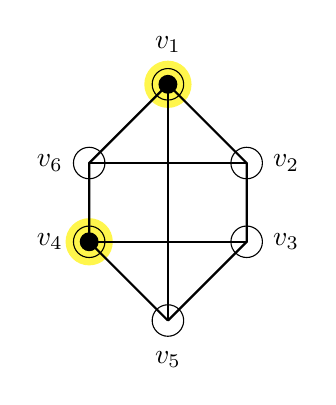
\begin{tikzpicture}[scale=1]
                \def\ver{0.12} %size of a vertex
                \def\xa{1}
                \def\ya{5}
                % highlight change
                \draw[fill=yellow, opacity=.7, draw=none] (\xa,\ya+3)  circle (0.3cm); % v1 ;
                \draw[fill=yellow, opacity=.7, draw=none] (\xa-1,\ya+1)  circle (0.3cm); % v4 ;

                %nodes
                \draw (\xa,\ya) circle (0.2cm);       % v5
                \draw (\xa+1,\ya+1) circle (0.2cm);   % v3
                \draw (\xa+1,\ya+2) circle (0.2cm);   % v2
                \draw (\xa,\ya+3) circle (0.2cm);     % v1
                \draw (\xa-1,\ya+2) circle (0.2cm);   % v6
                \draw (\xa-1,\ya+1) circle (0.2cm);   % v4

                %labels
                \node (1) at (\xa,\ya+3.5) {$v_1$};     % v1
                \node (2) at (\xa+1.5,\ya+2) {$v_2$};   % v2
                \node (3) at (\xa+1.5,\ya+1) {$v_3$};   % v3
                \node (5) at (\xa,\ya-0.5) {$v_5$};     % v5
                \node (4) at (\xa-1.5,\ya+1) {$v_4$};   % v4
                \node (6) at (\xa-1.5,\ya+2) {$v_6$};   % v6

                %token
                \path[fill] (\xa,\ya+3) circle (\ver);   % v1
                \path[fill] (\xa-1,\ya+1) circle (\ver); % v4

                %edges
                \draw[thick] (\xa,\ya)--(\xa+1,\ya+1)--(\xa+1,\ya+2)--(\xa,\ya+3)--(\xa-1,\ya+2)--(\xa-1,\ya+1)--(\xa,\ya) ; % contour
                \draw[thick] (\xa,\ya)--(\xa,\ya+3) ;       % v5 - v1
                \draw[thick] (\xa+1,\ya+1)--(\xa-1,\ya+1) ; % v3 - v4
                \draw[thick] (\xa+1,\ya+2)--(\xa-1,\ya+2) ; % v2 - v6
            \end{tikzpicture}
        \end{scaletikzpicturetowidth}
        \caption{A $3$-regular graph $G=(V,E)$ and initial independent set $I_1 = \{v_1, v_3\}$}
        \label{fig:s12}
    \end{subfigure}
    \begin{subfigure}[b]{0.4\textwidth}
        \begin{scaletikzpicturetowidth}{\textwidth}
            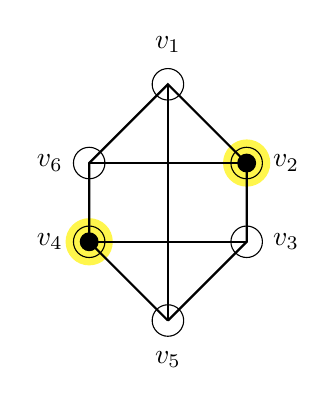
\begin{tikzpicture}[scale=1]
                \def\ver{0.12} %size of a vertex
                \def\xa{1}
                \def\ya{5}
                % highlight change
                \draw[fill=yellow, opacity=.7, draw=none] (\xa+1,\ya+2)  circle (0.3cm); % v2 ;
                \draw[fill=yellow, opacity=.7, draw=none] (\xa-1,\ya+1) circle (0.3cm); % v4 ;

                %nodes
                \draw (\xa,\ya) circle (0.2cm);       % v5
                \draw (\xa+1,\ya+1) circle (0.2cm);   % v3
                \draw (\xa+1,\ya+2) circle (0.2cm);   % v2
                \draw (\xa,\ya+3) circle (0.2cm);     % v1
                \draw (\xa-1,\ya+2) circle (0.2cm);   % v6
                \draw (\xa-1,\ya+1) circle (0.2cm);   % v4

                %labels
                \node (1) at (\xa,\ya+3.5) {$v_1$};     % v1
                \node (2) at (\xa+1.5,\ya+2) {$v_2$};   % v2
                \node (3) at (\xa+1.5,\ya+1) {$v_3$};   % v3
                \node (5) at (\xa,\ya-0.5) {$v_5$};     % v5
                \node (4) at (\xa-1.5,\ya+1) {$v_4$};   % v4
                \node (6) at (\xa-1.5,\ya+2) {$v_6$};   % v6

                %token
                \path[fill] (\xa+1,\ya+2) circle (\ver);   % v2
                \path[fill] (\xa-1,\ya+1) circle (\ver); % v4

                %edges
                \draw[thick] (\xa,\ya)--(\xa+1,\ya+1)--(\xa+1,\ya+2)--(\xa,\ya+3)--(\xa-1,\ya+2)--(\xa-1,\ya+1)--(\xa,\ya) ; % contour
                \draw[thick] (\xa,\ya)--(\xa,\ya+3) ;       % v5 - v1
                \draw[thick] (\xa+1,\ya+1)--(\xa-1,\ya+1) ; % v3 - v4
                \draw[thick] (\xa+1,\ya+2)--(\xa-1,\ya+2) ; % v2 - v6
            \end{tikzpicture}
        \end{scaletikzpicturetowidth}
        \caption{A $3$-regular graph $G=(V,E)$ and initial independent set $I_1 = \{v_1, v_3\}$}
        \label{fig:s13}
    \end{subfigure}
    \caption{Configuration-to-edge input instance}
    \label{fig:s2}
\end{figure}


\paragraph{St-Conn(S) problem in NCL.}

\paragraph{Can schaefer's dichotomy be applied to the 3-move subset sum reconfiguration problem i.e can we have a tight result for $k \leq 3$ and $k \geq 3 ? $}

\paragraph{Finding an optimal $k < 23$ for the colour classes of the exact cover problem. More en rapport avec le path in hypercube.}


%\section{Subset Sum where $S = W$}
\begin{theorem}{}Subset Sum Reconfiguration is strongly \NP-hard
\end{theorem}

\subsection{Preliminaries}
\begin{itemize}
    \item A packing $A_i$ is the subset of items in a set $A$ such that the total size of $A_i \leq$ capacity $c$ of a knapsack problem.
    \item The size of a packing $A_i = s(A_i)$.
    \item A packing doesn't necessarily satisfy a treshold $k$.
    \item Two packings are adjacent if their symmetric difference is of cardinality $1$.
    \item A reconfiguration sequence $P$ between two packings $A_0$ and $A_t$ is a sequence of packings $A_0, A_1, \dots, A_t$ such that $A_{i-1}$ and $A_i$ are adjacent $\forall i = 1, 2, \dots, t$.
    \item The minimum total size among all packings in $P$ is equal to $f(P)$ where $f(P) = min \{s(A_i) = A_i \in P\}$.
    \item For two packings $A_0$ and $A_t$ : $OPT(A_0, A_t) = max \{ f(P) : P$ is a reconfiguration sequence between $A_0$ and $A_t\}$.
\end{itemize}

\begin{defn}{(Subset Sum Reconfiguration).} Given an integer treshold $k$ and two packings $A_0$ and $A_t$, the Subset Sum reconfiguration problem is to determine whether $OPT(A_0, A_t) \geq k$.
\end{defn}

\begin{proof} $3$-partition problem $\leq_p$ Subset Sum Reconfiguration problem.

\begin{defn}{($3$-partition problem).} Given a positive integer bound $b$, a set $U$ of $3m$ elements $U_1,U_2, \dots, U_{3m}$, each element $u_i \in U$ has a positive size $s(u_i)$ such that $b/4 < s(u_i) < b/2$ and such that $\sum_{u \in U} s(u) = mb$. Then the $3$-partition problem is to determine whether $U$ can be partitioned in $m$ disjoint subsets
$U_1,U_2, \dots, U_{m}$ such that $\sum_{u \in U} s(u) = b$  $\forall j \in 1,\dots, m$.
\end{defn}

\paragraph{Reduction Construction} Given an instance of the $3$-partition problem, we construct the corresponding instance of the SUBSET SUM RECONFIGURATION problem.
\begin{itemize}
    \item From the given set $A$ and bound $b$, we will define a set $A$ consisting of $4m$ elements $a_1, a_2,\dots,a_{3m},b_1,b_2,\dots,b_m$.
    \item Let $s(a_i) = s(u_i)$ for each $i, 1 < i < 3m$. \\ Let $s(b_j) = b $ for each $j, 1 < j < m$. \\ Then each item $a_i$ corresponds to the element $u_i \in U$.
    \item The capacity $c$ will be $c.m$.
    \item The treshold $k = (m-1)b$.
    \item The two packings $A_0$ and $A_t$ are defined as follows :
    \begin{itemize}
        \item $A_0 = \{b_1, b_2,\dots, b_m\}$.
        \item $A_t = U$ \\ Both $A_0$ and $A_t$ are of total size $mb$ satisfying the constraint of the $3-partition$ problem.
    \end{itemize}
\end{itemize}

\paragraph{Correctness} Since $k = (m-1)b$ and $s(b_j) = b \forall j, 1 < j < m$, there exists a desired partition $\{U_1, U_2,\dots,u_m\}$ if and only if there exist a reconfiguration sequence $P$ between $A_0$ and $A_t$ with $f(P) = k = (m-1)b$ and hence $OPT(A_0, A_t) = (m-1)b \geq k$. \todo{Add more explanation to why}
\end{proof}

\begin{example}
    \begin{figure}[H]
        \begin{center}
            \begin{scaletikzpicturetowidth}{\textwidth}
                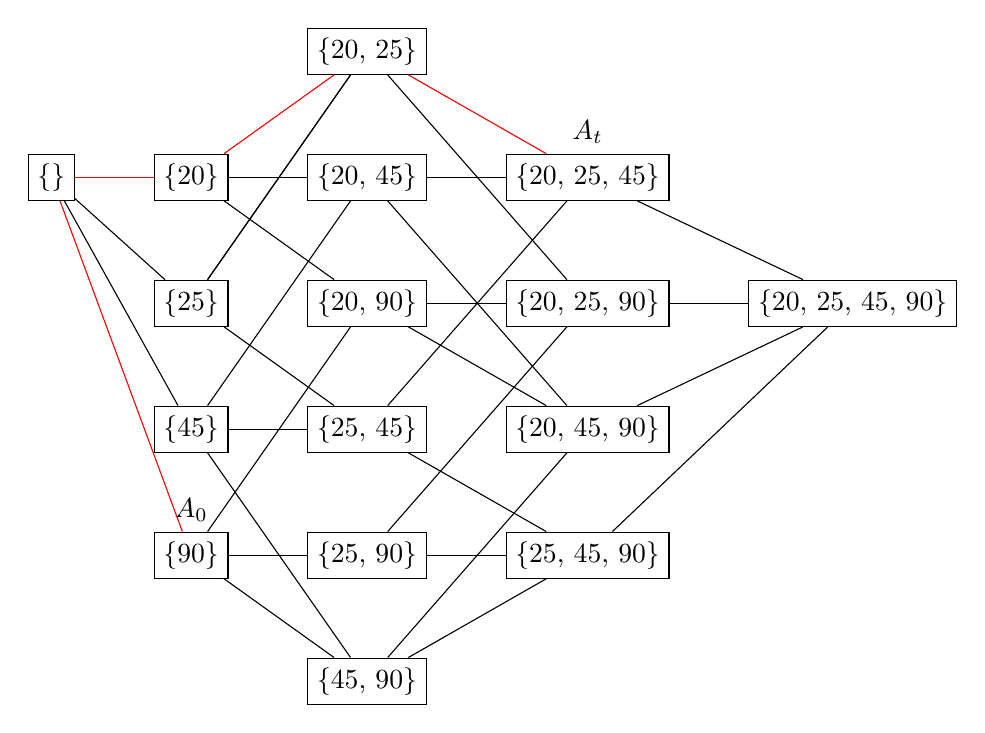
\begin{tikzpicture}[scale=1]
                    \node (16) [draw, rectangle] {\{\}};
                    \node (1) [right=of 16, draw, rectangle] {\{20\}};
                    \node (2) [below=of 1, draw, rectangle] {\{25\}};
                    \node (3) [below=of 2, draw, rectangle] {\{45\}};
                    \node (4) [label={$A_0$}, below=of 3, draw, rectangle] {\{90\}};
                    \node (5) [above right=of 1, draw, rectangle] {\{20, 25\}};
                    \node (6) [right=of 1, draw, rectangle] {\{20, 45\}};
                    \node (7) [right=of 2, draw, rectangle] {\{20, 90\}};
                    \node (8) [right=of 3, draw, rectangle] {\{25, 45\}};
                    \node (9) [right=of 4, draw, rectangle] {\{25, 90\}};
                    \node (10) [below right=of 4, draw, rectangle] {\{45, 90\}};
                    \node (11) [label={$A_t$},right=of 6, draw, rectangle] {\{20, 25, 45\}};
                    \node (12) [right=of 7, draw, rectangle] {\{20, 25, 90\}};
                    \node (13) [right=of 8, draw, rectangle] {\{20, 45, 90\}};
                    \node (14) [right=of 9, draw, rectangle] {\{25, 45, 90\}};
                    \node (15) [right=of 12, draw, rectangle] {\{20, 25, 45, 90\}};

                    \draw[-, red]  (16) to node [auto] {} (1);
                    \draw[-]  (16) to node [auto] {} (2);
                    \draw[-]  (16) to node [auto] {} (3);
                    \draw[-, red]  (16) to node [auto] {} (4);
                    \draw[-, red]  (1) to node [auto] {} (5);
                    \draw[-]  (1) to node [auto] {} (6);
                    \draw[-]  (1) to node [auto] {} (7);
                    \draw[-]  (2) to node [auto] {} (5);
                    \draw[-]  (2) to node [auto] {} (8);
                    \draw[-]  (2) to node [auto] {} (5);
                    \draw[-]  (3) to node [auto] {} (6);
                    \draw[-]  (3) to node [auto] {} (8);
                    \draw[-]  (3) to node [auto] {} (10);
                    \draw[-]  (4) to node [auto] {} (7);
                    \draw[-]  (4) to node [auto] {} (9);
                    \draw[-]  (4) to node [auto] {} (10);
                    \draw[-, red]  (5) to node [auto] {} (11);
                    \draw[-]  (5) to node [auto] {} (12);
                    \draw[-]  (6) to node [auto] {} (11);
                    \draw[-]  (6) to node [auto] {} (13);
                    \draw[-]  (7) to node [auto] {} (12);
                    \draw[-]  (7) to node [auto] {} (13);
                    \draw[-]  (8) to node [auto] {} (11);
                    \draw[-]  (8) to node [auto] {} (14);
                    \draw[-]  (9) to node [auto] {} (12);
                    \draw[-]  (9) to node [auto] {} (14);
                    \draw[-]  (10) to node [auto] {} (13);
                    \draw[-]  (10) to node [auto] {} (14);
                    \draw[-]  (11) to node [auto] {} (15);
                    \draw[-]  (12) to node [auto] {} (15);
                    \draw[-]  (13) to node [auto] {} (15);
                    \draw[-]  (14) to node [auto] {} (15);
                \end{tikzpicture}
            \end{scaletikzpicturetowidth}
        \end{center}
        \caption{All packings for $A$ = \{20,25,45\} and c = 90}\label{fig:specialCase}
    \end{figure}
\end{example}


\begin{itemize}
    \item $\mathcal{U} = \{v_1, v_2, v_3, v_4, v_5, v_6\} \cup \{t_1, t_2\}.$
    \item The set $\mathcal{S}$ :
    \begin{itemize}
        \item $\{v_1, v_3, v_5, v_6\}, \{v_2, v_3, v_5, v_6\},
        \{v_2, t_1\}, \{v_1, t_1\}, \{v_2, t_2\}, \{v_1, t_2\}, \\
        \{v_1, v_2, v_3, v_5, v_6, t_1\},  \{v_1, v_2, v_3, v_5, v_6, t_2\}$. \textcolor{gray}{$(v_1, v_2)$}

        \item $\{v_1, v_2, v_3, v_4, v_6\}, \{v_2, v_3, v_4, v_5, v_6\},
        \{v_5, t_1\}, \{v_1, t_1\}, \{t_2, v_5\}, \{v_1, t_2\}, \\
        \{v_1, v_2, v_3, v_4, v_5, v_6, t_1\}, \{v_1, v_2, v_3, v_4, v_5, v_6, t_2\}$.  \textcolor{gray}{$(v_1, v_5)$}

        \item $\{v_1, v_2, v_4, v_5\}, \{v_2, v_4, v_5, v_6\},
        \{v_6, t_1\}, \{v_1, t_1\}, \{v_6, t_2\}, \{v_1, t_2\}, \\
        \{v_1, v_2, v_4, v_5, v_6, t_1\}, \{v_1, v_2, v_4, v_5, v_6, t_2\}$.   \textcolor{gray}{$(v_1, v_6)$}

        \item $\{v_1, v_2, v_4, v_5, v_6\}, \{v_1, v_3, v_4, v_5, v_6\},
        \{v_3, t_1\}, \{v_2, t_1\}, \{v_3, t_2\}, \{v_2, t_2\}, \\
        \{v_1, v_2, v_3, v_4, v_5, v_6, t_1\}, \{v_1,v_2,v_3,v_4,v_5,v_6,t_2\}$. \textcolor{gray}{$(v_2, v_3)$}

        \item $\{v_1, v_2, v_3, v_4\}, \{v_1, v_3, v_4, v_6\},
        \{v_6, t_1\}, \{v_2, t_1\}, \{v_6, t_2\}, \{v_2, t_2\}, \\
        \{v_1, v_2, v_3, v_4, v_6, t_1\}, \{v_1, v_2, v_3, v_4, v_6, t_2\}$.   \textcolor{gray}{$(v_2, v_6)$}

        \item $\{v_2, v_3, v_5, v_6\}, \{v_2, v_4, v_5, v_6\},
        \{v_4, t_1\}, \{v_3, t_1\}, \{v_4, t_2\}, \{v_3, t_2\}, \\
        \{v_2, v_3, v_4, v_5, v_6, t_1\}, \{v_2, v_3, v_4, v_5, v_6, t_2\}$.   \textcolor{gray}{$(v_3, v_4)$}

        \item $\{v_1, v_2, v_3, v_4\}, \{v_1, v_2, v_4, v_5\},
        \{v_5, t_1\}, \{v_3, t_1\}, \{v_5, t_2\}, \{v_3, t_2\}, \\
        \{v_1, v_2, v_3, v_4, v_5, t_1\}, \{v_1, v_2, v_3, v_4, v_5, t_2\}$.  \textcolor{gray}{$(v_3, v_5)$}

        \item $\{v_1, v_3, v_4, v_6\}, \{v_1, v_3, v_5, v_6\},
        \{v_5, t_1\}, \{v_4, t_1\}, \{v_5, t_2\}, \{v_4, t_2\}, \\
        \{v_1, v_3, v_4, v_5, v_6, t_1\}, \{v_1, v_3, v_4, v_5, v_6, t_2\}$.  \textcolor{gray}{$(v_4, v_5)$}

        \item $\{v_1, v_2, v_3, v_4, v_5\}, \{v_1, v_2, v_3, v_5, v_6\},
        \{v_6, t_1\}, \{v_4, t_1\},  \{v_6, t_2\}, \{v_4, t_2\}, \\
        \{v_1, v_2, v_3, v_4, v_5, v_6, t_1\}, \{v_1, v_2, v_3, v_4, v_5, v_6, t_2\}$.  \textcolor{gray}{$(v_4, v_6)$}
    \end{itemize}
\end{itemize}
\end{example}


\begin{figure}[H]
\begin{center}
\begin{scaletikzpicturetowidth}{\textwidth}
\subfigure {
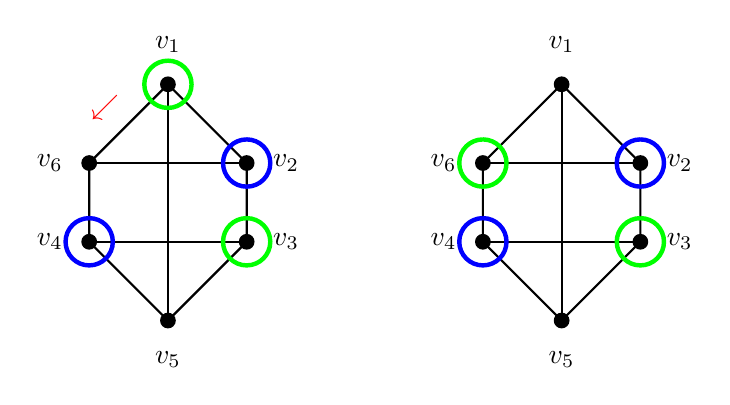
\begin{tikzpicture}[scale=1]
\def\ver{0.1} %size of a vertex
\def\xa{1}
\def\ya{5}
%---------------------Graph2------------------
%nodes
\def\xb{6}
\path[fill] (\xb,\ya) circle (\ver);       % v5
\path[fill] (\xb+1,\ya+1) circle (\ver);   % v3
\path[fill] (\xb+1,\ya+2) circle (\ver);   % v2
\path[fill] (\xb,\ya+3) circle (\ver);     % v1
\path[fill] (\xb-1,\ya+2) circle (\ver);   % v6
\path[fill] (\xb-1,\ya+1) circle (\ver);   % v4
%labels
\node (1) at (\xb,\ya+3.5) {$v_1$};     % v1
\node (2) at (\xb+1.5,\ya+2) {$v_2$};   % v2
\node (3) at (\xb+1.5,\ya+1) {$v_3$};   % v3
\node (5) at (\xb,\ya-0.5) {$v_5$};     % v5
\node (4) at (\xb-1.5,\ya+1) {$v_4$};   % v4
\node (6) at (\xb-1.5,\ya+2) {$v_6$};   % v6
%mid-slide
\node [color=red, ultra thick](7) at (5.2,7.7) {$\swarrow$};
%edges
\draw[thick] (\xb,\ya)--(\xb+1,\ya+1)--(\xb+1,\ya+2)--(\xb,\ya+3)--(\xb-1,\ya+2)--(\xb-1,\ya+1)--(\xb,\ya) ; % contour
\draw[thick] (\xb,\ya)--(\xb,\ya+3) ;       % v5 - v1
\draw[thick] (\xb+1,\ya+1)--(\xb-1,\ya+1) ; % v3 - v4
\draw[thick] (\xb+1,\ya+2)--(\xb-1,\ya+2) ; % v2 - v6
%independent sets
\draw[ultra thick,green] (\xb,\ya+3+ \ver+0.2) coordinate(a1)  arc (90:450:\ver +0.2) coordinate(a2);
\draw[ultra thick,green] (\xb+1,\ya+1+ \ver+0.2) coordinate(d1)  arc (90:450:\ver +0.2) coordinate(d2);
\draw[ultra thick,blue] (\xb-1,\ya+1+ \ver+0.2) coordinate(a1)  arc (90:450:\ver +0.2) coordinate(a2);
\draw[ultra thick,blue] (\xb+1,\ya+2+ \ver+0.2) coordinate(d1)  arc (90:450:\ver +0.2) coordinate(d2);

%---------------------Graph3-----------------------
%nodes
\def\xc{11}
\path[fill] (\xc,\ya) circle (\ver);       % v5
\path[fill] (\xc+1,\ya+1) circle (\ver);   % v3
\path[fill] (\xc+1,\ya+2) circle (\ver);   % v2
\path[fill] (\xc,\ya+3) circle (\ver);     % v1
\path[fill] (\xc-1,\ya+2) circle (\ver);   % v6
\path[fill] (\xc-1,\ya+1) circle (\ver);   % v4
%labels
\node (1) at (\xc,\ya+3.5) {$v_1$};     % v1
\node (2) at (\xc+1.5,\ya+2) {$v_2$};   % v2
\node (3) at (\xc+1.5,\ya+1) {$v_3$};   % v3
\node (5) at (\xc,\ya-0.5) {$v_5$};     % v5
\node (4) at (\xc-1.5,\ya+1) {$v_4$};   % v4
\node (6) at (\xc-1.5,\ya+2) {$v_6$};   % v6
%edges
\draw[thick] (\xc,\ya)--(\xc+1,\ya+1)--(\xc+1,\ya+2)--(\xc,\ya+3)--(\xc-1,\ya+2)--(\xc-1,\ya+1)--(\xc,\ya) ; % contour
\draw[thick] (\xc,\ya)--(\xc,\ya+3) ;       % v5 - v1
\draw[thick] (\xc+1,\ya+1)--(\xc-1,\ya+1) ; % v3 - v4
\draw[thick] (\xc+1,\ya+2)--(\xc-1,\ya+2) ; % v2 - v6
%independent sets
\draw[ultra thick,green] (\xc-1,\ya+2+ \ver+0.2) coordinate(a1)  arc (90:450:\ver +0.2) coordinate(a2);
\draw[ultra thick,green] (\xc+1,\ya+1+ \ver+0.2) coordinate(d1)  arc (90:450:\ver +0.2) coordinate(d2);
\draw[ultra thick,blue] (\xc-1,\ya+1+ \ver+0.2) coordinate(a1)  arc (90:450:\ver +0.2) coordinate(a2);
\draw[ultra thick,blue] (\xc+1,\ya+2+ \ver+0.2) coordinate(d1)  arc (90:450:\ver +0.2) coordinate(d2);
\end{tikzpicture}  }

\vspace{3em} % vertical space

\subfigure {
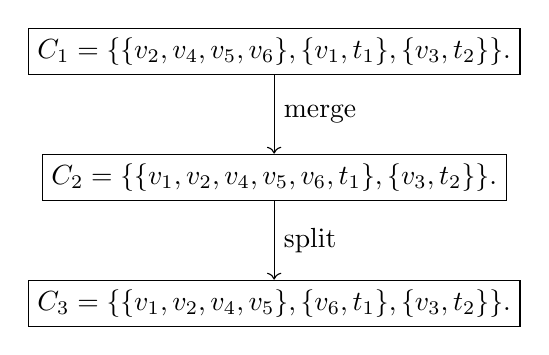
\begin{tikzpicture}[scale=1]
\node (1) [draw, rectangle] {$C_1 = \{ \{v_2, v_4, v_5, v_6\}, \{v_1, t_1\}, \{v_3, t_2\} \}$.};
\node (2) [below=of 1, draw, rectangle] {$C_2 = \{ \{v_1, v_2, v_4, v_5, v_6, t_1\}, \{v_3, t_2\} \}$.};
\node (3) [below=of 2, draw, rectangle] {$C_3 = \{ \{v_1, v_2, v_4, v_5\}, \{v_6, t_1\}, \{v_3, t_2\} \}$.};
\draw[->]  (1) to node [auto] {merge} (2);
\draw[->]  (2) to node [auto] {split} (3);
\end{tikzpicture} }
\end{scaletikzpicturetowidth}
\end{center}
\caption{}
\end{figure}


\begin{example}{Complete example of the reduction}
\begin{figure}[H]
\begin{center}
\begin{scaletikzpicturetowidth}{\textwidth}
\subfigure {
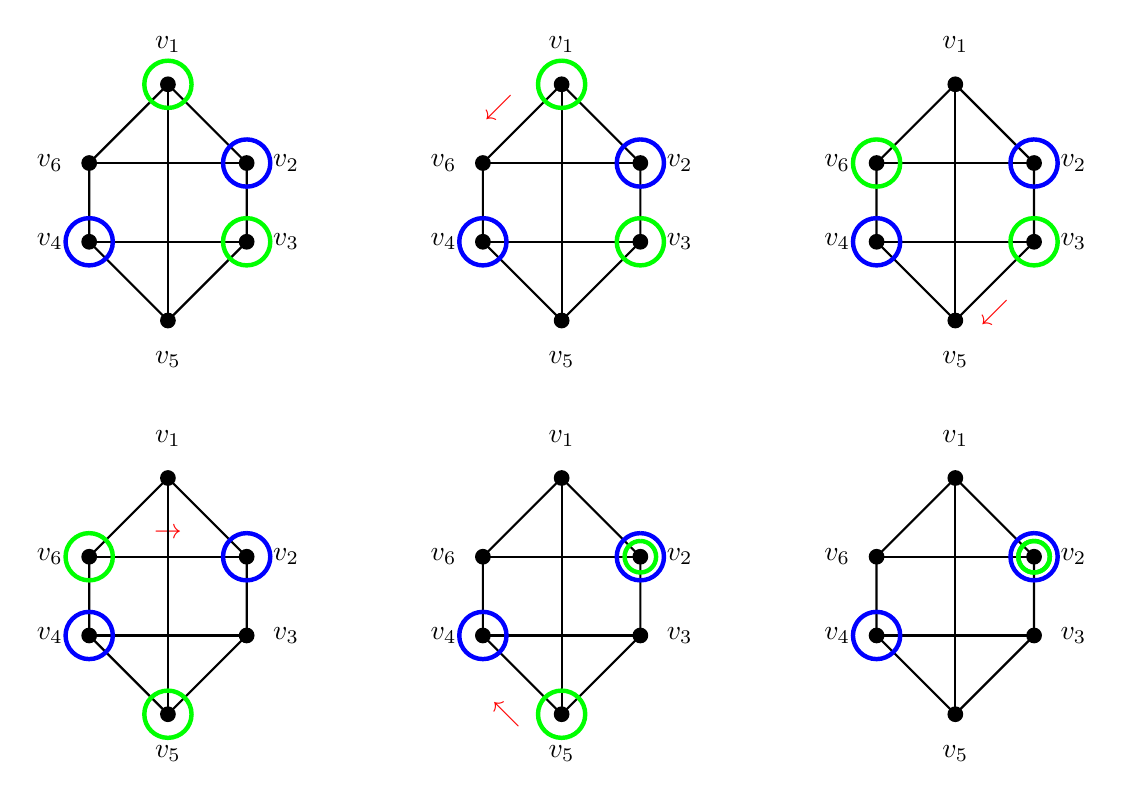
\begin{tikzpicture}[scale=1]

\def\ver{0.1} %size of a vertex
\def\xa{1}
\def\ya{5}
%--------------------- Graph 1 ---------------------
%nodes
\path[fill] (\xa,\ya) circle (\ver);       % v5
\path[fill] (\xa+1,\ya+1) circle (\ver);   % v3
\path[fill] (\xa+1,\ya+2) circle (\ver);   % v2
\path[fill] (\xa,\ya+3) circle (\ver);     % v1
\path[fill] (\xa-1,\ya+2) circle (\ver);   % v6
\path[fill] (\xa-1,\ya+1) circle (\ver);   % v4
%labels
\node (1) at (\xa,\ya+3.5) {$v_1$};     % v1
\node (2) at (\xa+1.5,\ya+2) {$v_2$};   % v2
\node (3) at (\xa+1.5,\ya+1) {$v_3$};   % v3
\node (5) at (\xa,\ya-0.5) {$v_5$};     % v5
\node (4) at (\xa-1.5,\ya+1) {$v_4$};   % v4
\node (6) at (\xa-1.5,\ya+2) {$v_6$};   % v6
%edges
\draw[thick] (\xa,\ya)--(\xa+1,\ya+1)--(\xa+1,\ya+2)--(\xa,\ya+3)--(\xa-1,\ya+2)--(\xa-1,\ya+1)--(\xa,\ya) ; % contour
\draw[thick] (\xa,\ya)--(\xa,\ya+3) ;       % v5 - v1
\draw[thick] (\xa+1,\ya+1)--(\xa-1,\ya+1) ; % v3 - v4
\draw[thick] (\xa+1,\ya+2)--(\xa-1,\ya+2) ; % v2 - v6
%independent sets
\draw[ultra thick,green] (\xa,\ya+3+ \ver+0.2) coordinate(a1)  arc (90:450:\ver +0.2) coordinate(a2);
\draw[ultra thick,green] (\xa+1,\ya+1+ \ver+0.2) coordinate(d1)  arc (90:450:\ver +0.2) coordinate(d2);
\draw[ultra thick,blue] (\xa-1,\ya+1+ \ver+0.2) coordinate(a1)  arc (90:450:\ver +0.2) coordinate(a2);
\draw[ultra thick,blue] (\xa+1,\ya+2+ \ver+0.2) coordinate(d1)  arc (90:450:\ver +0.2) coordinate(d2);


%---------------------Graph2------------------
%nodes
\def\xb{6}
\path[fill] (\xb,\ya) circle (\ver);       % v5
\path[fill] (\xb+1,\ya+1) circle (\ver);   % v3
\path[fill] (\xb+1,\ya+2) circle (\ver);   % v2
\path[fill] (\xb,\ya+3) circle (\ver);     % v1
\path[fill] (\xb-1,\ya+2) circle (\ver);   % v6
\path[fill] (\xb-1,\ya+1) circle (\ver);   % v4
%labels
\node (1) at (\xb,\ya+3.5) {$v_1$};     % v1
\node (2) at (\xb+1.5,\ya+2) {$v_2$};   % v2
\node (3) at (\xb+1.5,\ya+1) {$v_3$};   % v3
\node (5) at (\xb,\ya-0.5) {$v_5$};     % v5
\node (4) at (\xb-1.5,\ya+1) {$v_4$};   % v4
\node (6) at (\xb-1.5,\ya+2) {$v_6$};   % v6
%mid-slide
\node [color=red, ultra thick](7) at (5.2,7.7) {$\swarrow$};
%edges
\draw[thick] (\xb,\ya)--(\xb+1,\ya+1)--(\xb+1,\ya+2)--(\xb,\ya+3)--(\xb-1,\ya+2)--(\xb-1,\ya+1)--(\xb,\ya) ; % contour
\draw[thick] (\xb,\ya)--(\xb,\ya+3) ;       % v5 - v1
\draw[thick] (\xb+1,\ya+1)--(\xb-1,\ya+1) ; % v3 - v4
\draw[thick] (\xb+1,\ya+2)--(\xb-1,\ya+2) ; % v2 - v6
%independent sets
\draw[ultra thick,green] (\xb,\ya+3+ \ver+0.2) coordinate(a1)  arc (90:450:\ver +0.2) coordinate(a2);
\draw[ultra thick,green] (\xb+1,\ya+1+ \ver+0.2) coordinate(d1)  arc (90:450:\ver +0.2) coordinate(d2);
\draw[ultra thick,blue] (\xb-1,\ya+1+ \ver+0.2) coordinate(a1)  arc (90:450:\ver +0.2) coordinate(a2);
\draw[ultra thick,blue] (\xb+1,\ya+2+ \ver+0.2) coordinate(d1)  arc (90:450:\ver +0.2) coordinate(d2);

%---------------------Graph3-----------------------
%nodes
\def\xc{11}
\path[fill] (\xc,\ya) circle (\ver);       % v5
\path[fill] (\xc+1,\ya+1) circle (\ver);   % v3
\path[fill] (\xc+1,\ya+2) circle (\ver);   % v2
\path[fill] (\xc,\ya+3) circle (\ver);     % v1
\path[fill] (\xc-1,\ya+2) circle (\ver);   % v6
\path[fill] (\xc-1,\ya+1) circle (\ver);   % v4
%labels
\node (1) at (\xc,\ya+3.5) {$v_1$};     % v1
\node (2) at (\xc+1.5,\ya+2) {$v_2$};   % v2
\node (3) at (\xc+1.5,\ya+1) {$v_3$};   % v3
\node (5) at (\xc,\ya-0.5) {$v_5$};     % v5
\node (4) at (\xc-1.5,\ya+1) {$v_4$};   % v4
\node (6) at (\xc-1.5,\ya+2) {$v_6$};   % v6
%mid-slide
\node [color=red, ultra thick](7) at (\xc+0.5,\ya+0.1) {$\swarrow$};
%edges
\draw[thick] (\xc,\ya)--(\xc+1,\ya+1)--(\xc+1,\ya+2)--(\xc,\ya+3)--(\xc-1,\ya+2)--(\xc-1,\ya+1)--(\xc,\ya) ; % contour
\draw[thick] (\xc,\ya)--(\xc,\ya+3) ;       % v5 - v1
\draw[thick] (\xc+1,\ya+1)--(\xc-1,\ya+1) ; % v3 - v4
\draw[thick] (\xc+1,\ya+2)--(\xc-1,\ya+2) ; % v2 - v6
%independent sets
\draw[ultra thick,green] (\xc-1,\ya+2+ \ver+0.2) coordinate(a1)  arc (90:450:\ver +0.2) coordinate(a2);
\draw[ultra thick,green] (\xc+1,\ya+1+ \ver+0.2) coordinate(d1)  arc (90:450:\ver +0.2) coordinate(d2);
\draw[ultra thick,blue] (\xc-1,\ya+1+ \ver+0.2) coordinate(a1)  arc (90:450:\ver +0.2) coordinate(a2);
\draw[ultra thick,blue] (\xc+1,\ya+2+ \ver+0.2) coordinate(d1)  arc (90:450:\ver +0.2) coordinate(d2);

%--------------------- Graph 4 ---------------------
\def\ya{0}
%nodes
\path[fill] (\xa,\ya) circle (\ver);       % v5
\path[fill] (\xa+1,\ya+1) circle (\ver);   % v3
\path[fill] (\xa+1,\ya+2) circle (\ver);   % v2
\path[fill] (\xa,\ya+3) circle (\ver);     % v1
\path[fill] (\xa-1,\ya+2) circle (\ver);   % v6
\path[fill] (\xa-1,\ya+1) circle (\ver);   % v4
%labels
\node (1) at (\xa,\ya+3.5) {$v_1$};     % v1
\node (2) at (\xa+1.5,\ya+2) {$v_2$};   % v2
\node (3) at (\xa+1.5,\ya+1) {$v_3$};   % v3
\node (5) at (\xa,\ya-0.5) {$v_5$};     % v5
\node (4) at (\xa-1.5,\ya+1) {$v_4$};   % v4
\node (6) at (\xa-1.5,\ya+2) {$v_6$};   % v6
%mid-slide
\node [color=red, ultra thick](7) at (\xa,\ya+2.3) {$\rightarrow$};
%edges
\draw[thick] (\xa,\ya)--(\xa+1,\ya+1)--(\xa+1,\ya+2)--(\xa,\ya+3)--(\xa-1,\ya+2)--(\xa-1,\ya+1)--(\xa,\ya) ; % contour
\draw[thick] (\xa,\ya)--(\xa,\ya+3) ;       % v5 - v1
\draw[thick] (\xa+1,\ya+1)--(\xa-1,\ya+1) ; % v3 - v4
\draw[thick] (\xa+1,\ya+2)--(\xa-1,\ya+2) ; % v2 - v6
%independent sets
\draw[ultra thick,green] (\xa-1,\ya+2+ \ver+0.2) coordinate(a1)  arc (90:450:\ver +0.2) coordinate(a2); % v6
\draw[ultra thick,green] (\xa,\ya+ \ver+0.2) coordinate(d1)  arc (90:450:\ver +0.2) coordinate(d2); % v5
\draw[ultra thick,blue] (\xa-1,\ya+1+ \ver+0.2) coordinate(a1)  arc (90:450:\ver +0.2) coordinate(a2);
\draw[ultra thick,blue] (\xa+1,\ya+2+ \ver+0.2) coordinate(d1)  arc (90:450:\ver +0.2) coordinate(d2);

%---------------------Graph 5 ------------------
%nodes
\def\xb{6}
\path[fill] (\xb,\ya) circle (\ver);       % v5
\path[fill] (\xb+1,\ya+1) circle (\ver);   % v3
\path[fill] (\xb+1,\ya+2) circle (\ver);   % v2
\path[fill] (\xb,\ya+3) circle (\ver);     % v1
\path[fill] (\xb-1,\ya+2) circle (\ver);   % v6
\path[fill] (\xb-1,\ya+1) circle (\ver);   % v4
%labels
\node (1) at (\xb,\ya+3.5) {$v_1$};     % v1
\node (2) at (\xb+1.5,\ya+2) {$v_2$};   % v2
\node (3) at (\xb+1.5,\ya+1) {$v_3$};   % v3
\node (5) at (\xb,\ya-0.5) {$v_5$};     % v5
\node (4) at (\xb-1.5,\ya+1) {$v_4$};   % v4
\node (6) at (\xb-1.5,\ya+2) {$v_6$};   % v6
%mid-slide
\node [color=red, ultra thick](7) at (\xb-0.7,\ya) {$\nwarrow$};
%edges
\draw[thick] (\xb,\ya)--(\xb+1,\ya+1)--(\xb+1,\ya+2)--(\xb,\ya+3)--(\xb-1,\ya+2)--(\xb-1,\ya+1)--(\xb,\ya) ; % contour
\draw[thick] (\xb,\ya)--(\xb,\ya+3) ;       % v5 - v1
\draw[thick] (\xb+1,\ya+1)--(\xb-1,\ya+1) ; % v3 - v4
\draw[thick] (\xb+1,\ya+2)--(\xb-1,\ya+2) ; % v2 - v6
%independent sets
\draw[ultra thick,green] (\xb+1,\ya+2+ \ver+0.1) coordinate(a1)  arc (90:450:\ver +0.1) coordinate(a2);   % v4
\draw[ultra thick,green] (\xb,\ya+ \ver+0.2) coordinate(d1)  arc (90:450:\ver +0.2) coordinate(d2);       % v5
\draw[ultra thick,blue] (\xb-1,\ya+1+ \ver+0.2) coordinate(a1)  arc (90:450:\ver +0.2) coordinate(a2);    % v4
\draw[ultra thick,blue] (\xb+1,\ya+2+ \ver+0.2) coordinate(d1)  arc (90:450:\ver +0.2) coordinate(d2);    % v2

%---------------------Graph 6 -----------------------
%nodes
\def\xc{11}
\path[fill] (\xc,\ya) circle (\ver);       % v5
\path[fill] (\xc+1,\ya+1) circle (\ver);   % v3
\path[fill] (\xc+1,\ya+2) circle (\ver);   % v2
\path[fill] (\xc,\ya+3) circle (\ver);     % v1
\path[fill] (\xc-1,\ya+2) circle (\ver);   % v6
\path[fill] (\xc-1,\ya+1) circle (\ver);   % v4
%labels
\node (1) at (\xc,\ya+3.5) {$v_1$};     % v1
\node (2) at (\xc+1.5,\ya+2) {$v_2$};   % v2
\node (3) at (\xc+1.5,\ya+1) {$v_3$};   % v3
\node (5) at (\xc,\ya-0.5) {$v_5$};     % v5
\node (4) at (\xc-1.5,\ya+1) {$v_4$};   % v4
\node (6) at (\xc-1.5,\ya+2) {$v_6$};   % v6
%edges
\draw[thick] (\xc,\ya)--(\xc+1,\ya+1)--(\xc+1,\ya+2)--(\xc,\ya+3)--(\xc-1,\ya+2)--(\xc-1,\ya+1)--(\xc,\ya) ; % contour
\draw[thick] (\xc,\ya)--(\xc,\ya+3) ;       % v5 - v1
\draw[thick] (\xc+1,\ya+1)--(\xc-1,\ya+1) ; % v3 - v4
\draw[thick] (\xc+1,\ya+2)--(\xc-1,\ya+2) ; % v2 - v6
%independent sets
\draw[ultra thick,green] (\xc+1,\ya+2+ \ver+0.1) coordinate(a1)  arc (90:450:\ver +0.1) coordinate(a2);   % v4
\draw[ultra thick,green] (\xc+1,\ya+2+ \ver+0.1) coordinate(d1)  arc (90:450:\ver +0.1) coordinate(d2);   % v2
\draw[ultra thick,blue] (\xc-1,\ya+1+ \ver+0.2) coordinate(a1)  arc (90:450:\ver +0.2) coordinate(a2);    % v4
\draw[ultra thick,blue] (\xc+1,\ya+2+ \ver+0.2) coordinate(d1)  arc (90:450:\ver +0.2) coordinate(d2);    % v2

\end{tikzpicture} }

\vspace{3em} % vertical space

\subfigure {
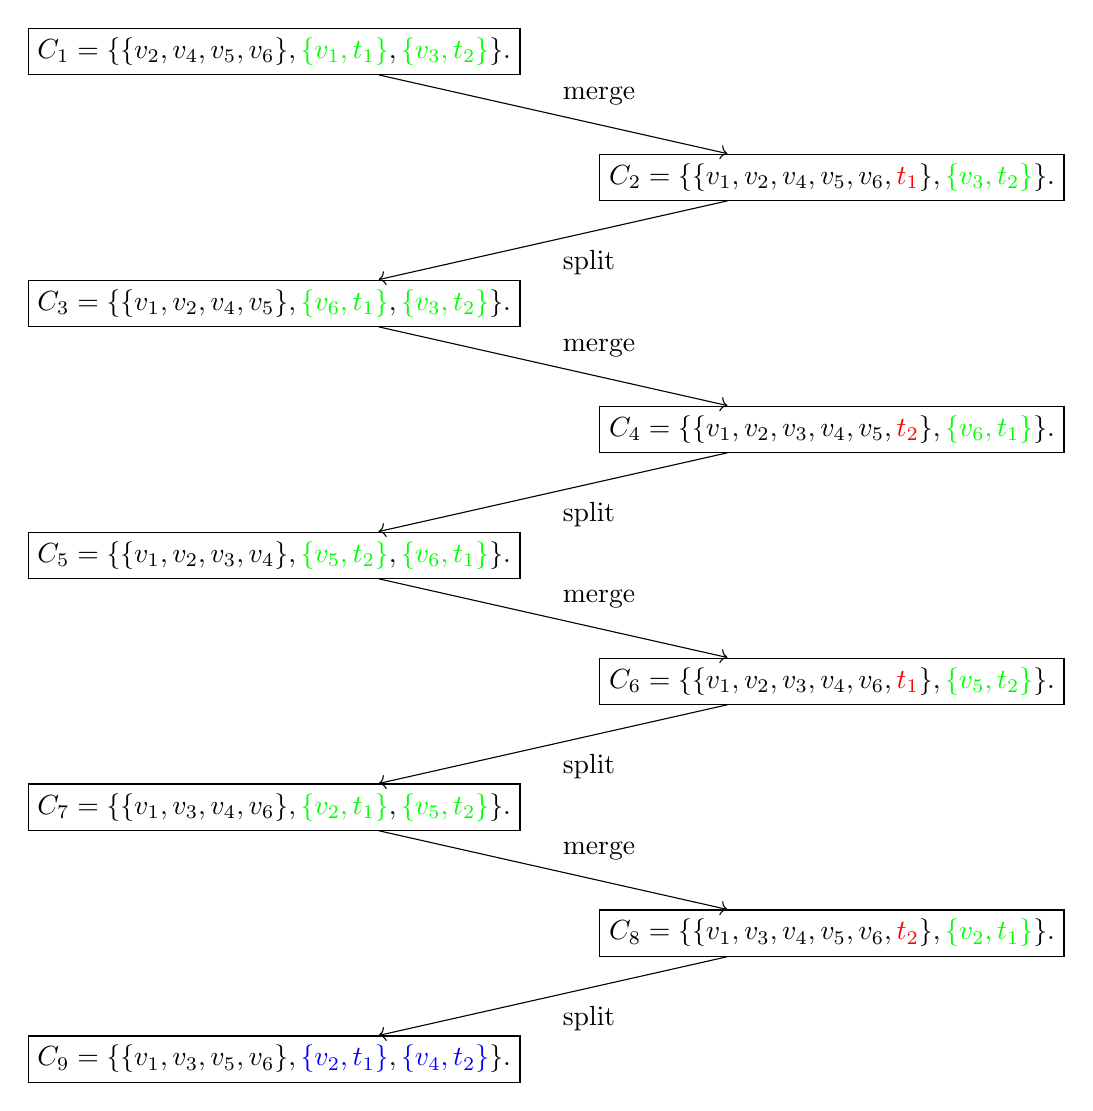
\begin{tikzpicture}[scale=1]
\node (1) [draw, rectangle] {$C_1 = \{ \{v_2, v_4, v_5, v_6\}, \textcolor{green}{\{v_1, t_1\}}, \textcolor{green}{\{v_3, t_2\}} \}$.};
\node (2) [below right=of 1, draw, rectangle] {$C_2 = \{ \{v_1, v_2, v_4, v_5, v_6, \textcolor{red}{t_1}\}, \textcolor{green}{\{v_3, t_2\}} \}$.};
\node (3) [below left=of 2, draw, rectangle] {$C_3 = \{ \{v_1, v_2, v_4, v_5\}, \textcolor{green}{\{v_6, t_1\}}, \textcolor{green}{\{v_3, t_2\}} \}$.};
\node (4) [below right=of 3, draw, rectangle] {$C_4 = \{ \{v_1, v_2, v_3, v_4, v_5, \textcolor{red}{t_2}\}, \textcolor{green}{\{v_6, t_1\}} \}$.};
\node (5) [below left=of 4, draw, rectangle] {$C_5 = \{ \{v_1, v_2, v_3, v_4\}, \textcolor{green}{\{v_5, t_2\}}, \textcolor{green}{\{v_6, t_1\}} \}$.};
\node (6) [below right=of 5, draw, rectangle] {$C_6 = \{ \{v_1, v_2, v_3, v_4,v_6,\textcolor{red}{t_1}\}, \textcolor{green}{\{v_5, t_2\}} \}$.};
\node (7) [below left=of 6, draw, rectangle] {$C_7 = \{ \{v_1, v_3, v_4,v_6\}, \textcolor{green}{\{v_2, t_1\}}, \textcolor{green}{\{v_5, t_2\}}\}$.};
\node (8) [below right=of 7, draw, rectangle] {$C_8 = \{ \{v_1, v_3, v_4, v_5, v_6, \textcolor{red}{t_2}\}, \textcolor{green}{\{v_2, t_1\}} \}$.};
\node (9) [below left=of 8, draw, rectangle] {$C_9 = \{ \{v_1, v_3, v_5, v_6\}, \textcolor{blue}{\{v_2, t_1\}}, \textcolor{blue}{\{v_4, t_2\}} \}$.};
\draw[->]  (1) to node [auto] {merge} (2);
\draw[->]  (2) to node [auto] {split} (3);
\draw[->]  (3) to node [auto] {merge} (4);
\draw[->]  (4) to node [auto] {split} (5);
\draw[->]  (5) to node [auto] {merge} (6);
\draw[->]  (6) to node [auto] {split} (7);
\draw[->]  (7) to node [auto] {merge} (8);
\draw[->]  (8) to node [auto] {split} (9);
\end{tikzpicture} }
\end{scaletikzpicturetowidth}
\end{scaletikzpicturetowidth}
\end{center}
\caption{}
\end{figure}
\end{example}



%%%%%%%%%%%%%%%%%%%%%%%%%%%%%%%%%%%%%%%% BEGINING OF A FIGURE : All possible moves of an AND vertex %%%%%%%%%%%%%%%%%%%%%%%%%%%%%%%%%%%%%%%%%%%
\begin{figure}[H]
\begin{center}
\begin{scaletikzpicturetowidth}{\textwidth}
\begin{tikzpicture}[scale=0.7]
% v1
\def\xa{0}
\def\ya{0}
% v2
\def\xb{\xa-3}
\def\yb{\ya+3}
% v3
\def\xc{\xa+3}
\def\yc{\ya+3}
% v4
\def\xd{\xa}
\def\yd{\ya+6}
% v5
\def\xe{\xa}
\def\ye{\ya-4}
%labels
\node (1) at (\xa+2,\ya) {$f_1$};
\node (2) at (\xb-2,\yb) {$f_2$};
\node (3) at (\xc+2,\yc) {$f_3$};
\node (5) at (\xd+2,\yd) {$f_4$};
\node (4) at (\xe+2,\ye) {$f_0$};
% f_1 arrows
\draw[middlearrow={<}, red] (\xa, \ya) -- (\xa+0.9, \ya-0.8);
\draw[middlearrow={<}, red] (\xa, \ya) -- (\xa-1, \ya-0.8);
\draw[middlearrow={<}, blue] (\xa, \ya) -- (\xa, \ya+1);
\draw[ultra thick, -, blue] (\xa, \ya) -- (\xa, \ya+1);
\draw[ultra thick, -, red] (\xa, \ya) -- (\xa+0.9, \ya-0.8);
\draw[ultra thick, -, red] (\xa, \ya) -- (\xa-1, \ya-0.8);
\path[fill=none, draw, ultra thick, dotted] (\xa,\ya) circle (\ver+1.2);     %f1
% f_2 arrows
\draw[middlearrow={>}, red] (\xb, \yb) --(\xb-0.9, \yb-0.8);
\draw[middlearrow={<}, red] (\xb, \yb) --(\xb+0.9, \yb-0.8);
\draw[middlearrow={<}, blue] (\xb, \yb) --(\xb, \yb+1);
\draw[ultra thick, -, red] (\xb, \yb) --(\xb-0.9, \yb-0.8);
\draw[ultra thick, -, red] (\xb, \yb) --(\xb+0.9, \yb-0.8);
\draw[ultra thick, -, blue] (\xb, \yb) --(\xb, \yb+1);
\path[fill=none, draw, ultra thick, dotted] (\xb,\yb) circle (\ver+1.2);     %f2
% f_3  arrows
\draw[middlearrow={<}, red] (\xc, \yc) --(\xc-0.9, \yc-0.8);
\draw[middlearrow={>}, red] (\xc, \yc) --(\xc+0.9, \yc-0.8);
\draw[middlearrow={<}, blue] (\xc, \yc) --(\xc, \yc+1);
\draw[ultra thick, -, red] (\xc, \yc) --(\xc-0.9, \yc-0.8);
\draw[ultra thick, -, red] (\xc, \yc) --(\xc+0.9, \yc-0.8);
\draw[ultra thick, -, blue] (\xc, \yc) --(\xc, \yc+1);
\path[fill=none, draw, ultra thick, dotted] (\xc,\yc) circle (\ver+1.2);     %f3
% f_4  arrows
\draw[middlearrow={>}, red] (\xd, \yd) --(\xd-0.9, \yd-0.8);
\draw[middlearrow={>}, red] (\xd, \yd) --(\xd+0.9, \yd-0.8);
\draw[middlearrow={<}, blue] (\xd, \yd) --(\xd, \yd+1);
\draw[ultra thick, -, red] (\xd, \yd) --(\xd-0.9, \yd-0.8);
\draw[ultra thick, -, red] (\xd, \yd) --(\xd+0.9, \yd-0.8);
\draw[ultra thick, -, blue] (\xd, \yd) --(\xd, \yd+1);
\path[fill=none, draw, ultra thick, dotted] (\xd,\yd) circle (\ver+1.2);     %f4
% f_0  arrows
\draw[middlearrow={<}, red] (\xe, \ye) --(\xe-0.9, \ye-0.8);
\draw[middlearrow={<}, red] (\xe, \ye) --(\xe+0.9, \ye-0.8);
\draw[middlearrow={>}, blue] (\xe, \ye) --(\xe, \ye+1);
\draw[ultra thick, -, red] (\xe, \ye) --(\xe-0.9, \ye-0.8);
\draw[ultra thick, -, red] (\xe, \ye) --(\xe+0.9, \ye-0.8);
\draw[ultra thick, -, blue] (\xe, \ye) --(\xe, \ye+1);
\path[fill=none, draw, ultra thick, dotted] (\xe,\ye) circle (\ver+1.2);     %f0
%relations
\draw[ultra thick, <->] (\xe,\ye+1.4) -- (\xa,\ya-1.4);
\draw[ultra thick, <->] (\xa+1,\ya+1) -- (\xc-1,\yc-1);
\draw[ultra thick, <->] (\xa-1,\ya+1) -- (\xb+1,\yb-1);
\draw[ultra thick, <->] (\xc-1,\yc+1) -- (\xd+1,\yd-1);
\draw[ultra thick, <->] (\xd-1,\yd-1) -- (\xb+1,\yb+1);
%graph G : Nodes fill
\path[fill] (\xa,\ya) circle (\ver);     %f1
\path[fill] (\xb,\yb) circle (\ver);     %f2
\path[fill] (\xc,\yc) circle (\ver);     %f3
\path[fill] (\xd,\yd) circle (\ver);     %f4
\path[fill] (\xe,\ye) circle (\ver);     %f0
\end{tikzpicture}
\end{scaletikzpicturetowidth}
\end{center}
\caption{All the possible orientations of edges of an AND vertex.}
\label{fig:and_all_possible_moves}
\end{figure}
%%%%%%%%%%%%%%%%%%%%%%%%%%%%%%%%%%%%%%%%%%% ENDING OF A FIGURE %%%%%%%%%%%%%%%%%%%%%%%%%%%%%%%%%%%%%%%

%%%%%%%%%%%%%%%%%%%%%%%%%%%%%%%%%%%%%% BEGINING OF A FIGURE : All possible moves of an OR vertex  %%%%%%%%%%%%%%%%%%%%%%%%%%%%%%%%%%%%%
\begin{figure}[H]
\begin{center}
\begin{scaletikzpicturetowidth}{\textwidth}
\begin{tikzpicture}[scale=0.7]
% v1
\def\xa{0}
\def\ya{0}
% v2
\def\xb{\xa-3}
\def\yb{\ya+3}
% v3
\def\xc{\xa+3}
\def\yc{\ya+3}
% v4
\def\xd{\xa}
\def\yd{\ya+6}
% v5
\def\xe{\xa}
\def\ye{\ya-4}
% v6
\def\xf{\xa-3}
\def\yf{\ya-7}
% v7
\def\xg{\xa+3}
\def\yg{\ya-7}
%labels
\node (1) at (\xa+2,\ya) {$f_1$};
\node (2) at (\xb-2,\yb) {$f_2$};
\node (3) at (\xc+2,\yc) {$f_3$};
\node (5) at (\xd+2,\yd) {$f_4$};
\node (4) at (\xe+2,\ye) {$f_0$};
\node (6) at (\xf-2,\yf) {$f_6$};
\node (7) at (\xg+2,\yg) {$f_7$};
% f_1 arrows
\draw[middlearrow={<}, blue] (\xa, \ya) -- (\xa+0.9, \ya-0.8);
\draw[middlearrow={<}, blue] (\xa, \ya) -- (\xa-1, \ya-0.8);
\draw[middlearrow={<}, blue] (\xa, \ya) -- (\xa, \ya+1);
\draw[ultra thick, -, blue] (\xa, \ya) -- (\xa, \ya+1);
\draw[ultra thick, -, blue] (\xa, \ya) -- (\xa+0.9, \ya-0.8);
\draw[ultra thick, -, blue] (\xa, \ya) -- (\xa-1, \ya-0.8);
\path[fill=none, draw, ultra thick, dotted] (\xa,\ya) circle (\ver+1.2);     %f1
% f_2 arrows
\draw[middlearrow={>}, blue] (\xb, \yb) --(\xb-0.9, \yb-0.8);
\draw[middlearrow={<}, blue] (\xb, \yb) --(\xb+0.9, \yb-0.8);
\draw[middlearrow={<}, blue] (\xb, \yb) --(\xb, \yb+1);
\draw[ultra thick, -, blue] (\xb, \yb) --(\xb-0.9, \yb-0.8);
\draw[ultra thick, -, blue] (\xb, \yb) --(\xb+0.9, \yb-0.8);
\draw[ultra thick, -, blue] (\xb, \yb) --(\xb, \yb+1);
\path[fill=none, draw, ultra thick, dotted] (\xb,\yb) circle (\ver+1.2);     %f2
% f_3  arrows
\draw[middlearrow={<}, blue] (\xc, \yc) --(\xc-0.9, \yc-0.8);
\draw[middlearrow={>}, blue] (\xc, \yc) --(\xc+0.9, \yc-0.8);
\draw[middlearrow={<}, blue] (\xc, \yc) --(\xc, \yc+1);
\draw[ultra thick, -, blue] (\xc, \yc) --(\xc-0.9, \yc-0.8);
\draw[ultra thick, -, blue] (\xc, \yc) --(\xc+0.9, \yc-0.8);
\draw[ultra thick, -, blue] (\xc, \yc) --(\xc, \yc+1);
\path[fill=none, draw, ultra thick, dotted] (\xc,\yc) circle (\ver+1.2);     %f3
% f_4  arrows
\draw[middlearrow={>}, blue] (\xd, \yd) --(\xd-0.9, \yd-0.8);
\draw[middlearrow={>}, blue] (\xd, \yd) --(\xd+0.9, \yd-0.8);
\draw[middlearrow={<}, blue] (\xd, \yd) --(\xd, \yd+1);
\draw[ultra thick, -, blue] (\xd, \yd) --(\xd-0.9, \yd-0.8);
\draw[ultra thick, -, blue] (\xd, \yd) --(\xd+0.9, \yd-0.8);
\draw[ultra thick, -, blue] (\xd, \yd) --(\xd, \yd+1);
\path[fill=none, draw, ultra thick, dotted] (\xd,\yd) circle (\ver+1.2);     %f4
% f_0  arrows
\draw[middlearrow={<}, blue] (\xe, \ye) --(\xe-0.9, \ye-0.8);
\draw[middlearrow={<}, blue] (\xe, \ye) --(\xe+0.9, \ye-0.8);
\draw[middlearrow={>}, blue] (\xe, \ye) --(\xe, \ye+1);
\draw[ultra thick, -, blue] (\xe, \ye) --(\xe-0.9, \ye-0.8);
\draw[ultra thick, -, blue] (\xe, \ye) --(\xe+0.9, \ye-0.8);
\draw[ultra thick, -, blue] (\xe, \ye) --(\xe, \ye+1);
\path[fill=none, draw, ultra thick, dotted] (\xe,\ye) circle (\ver+1.2);     %f0
% f_6 arrows
\draw[middlearrow={>}, blue] (\xf, \yf) --(\xf-0.9, \yf-0.8);
\draw[middlearrow={<}, blue] (\xf, \yf) --(\xf+0.9, \yf-0.8);
\draw[middlearrow={>}, blue] (\xf, \yf) --(\xf, \yf+1);
\draw[ultra thick, -, blue] (\xf, \yf) --(\xf-0.9, \yf-0.8);
\draw[ultra thick, -, blue] (\xf, \yf) --(\xf+0.9, \yf-0.8);
\draw[ultra thick, -, blue] (\xf, \yf) --(\xf, \yf+1);
\path[fill=none, draw, ultra thick, dotted] (\xf,\yf) circle (\ver+1.2);     %f6
% f_7 arrows
\draw[middlearrow={<}, blue] (\xg, \yg) --(\xg-0.9, \yg-0.8);
\draw[middlearrow={>}, blue] (\xg, \yg) --(\xg+0.9, \yg-0.8);
\draw[middlearrow={>}, blue] (\xg, \yg) --(\xg, \yg+1);
\draw[ultra thick, -, blue] (\xg, \yg) --(\xg-0.9, \yg-0.8);
\draw[ultra thick, -, blue] (\xg, \yg) --(\xg+0.9, \yg-0.8);
\draw[ultra thick, -, blue] (\xg, \yg) --(\xg, \yg+1);
\path[fill=none, draw, ultra thick, dotted] (\xg,\yg) circle (\ver+1.2);     %f7
%relations
\draw[ultra thick, <->] (\xe,\ye+1.4) -- (\xa,\ya-1.4);
\draw[ultra thick, <->] (\xa+1,\ya+1) -- (\xc-1,\yc-1);
\draw[ultra thick, <->] (\xa-1,\ya+1) -- (\xb+1,\yb-1);
\draw[ultra thick, <->] (\xc-1,\yc+1) -- (\xd+1,\yd-1);
\draw[ultra thick, <->] (\xd-1,\yd-1) -- (\xb+1,\yb+1);
\draw[ultra thick, <->] (\xe-1,\ye-1) -- (\xf+1,\yf+1);
\draw[ultra thick, <->] (\xe+1,\ye-1) -- (\xg-1,\yg+1);
%graph G : Nodes fill
\path[fill] (\xa,\ya) circle (\ver);     %f1
\path[fill] (\xb,\yb) circle (\ver);     %f2
\path[fill] (\xc,\yc) circle (\ver);     %f3
\path[fill] (\xd,\yd) circle (\ver);     %f4
\path[fill] (\xe,\ye) circle (\ver);     %f0
\path[fill] (\xf,\yf) circle (\ver);     %f6
\path[fill] (\xg,\yg) circle (\ver);     %f7
\end{tikzpicture}
\end{scaletikzpicturetowidth}
\end{center}
\caption{All the possible orientations of edges of an OR vertex.}
\label{fig:or_all_possible_moves}
\end{figure}
%%%%%%%%%%%%%%%%%%%%%%%%%%%%%%%%%%%%%%%%%%%%%%%% ENDING OF A FIGURE %%%%%%%%%%%%%%%%%%%%%%%%%%%%%%%%%%%%%%%%%%%%%%%%


%----------------------------------------------------------------------------------------
%	THESIS CONTENT - APPENDICES
%----------------------------------------------------------------------------------------

    \appendix % Cue to tell LaTeX that the following "chapters" are Appendices

% Include the appendices of the thesis as separate files from the Appendices folder
% Uncomment the lines as you write the Appendices

%% Appendix A

\chapter{Frequently Asked Questions} % Main appendix title

\label{AppendixA} % For referencing this appendix elsewhere, use \ref{AppendixA}

\section{How do I change the labelleds of links?}

The  of links can be changed to your liking using:

{\small\verb!\hypersetup{url=red}!}, or

{\small\verb!\hypersetup{cite=green}!}, or

{\small\verb!\hypersetup{all=blue}!}.

\noindent If you want to completely hide the links, you can use:

{\small\verb!\hypersetup{alls=.}!}, or even better:

{\small\verb!\hypersetup{hidelinks}!}.

\noindent If you want to have obvious links in the PDF but not the printed text, use:

{\small\verb!\hypersetup{links=false}!}.

%\include{Appendices/AppendixB}
%\include{Appendices/AppendixC}

%----------------------------------------------------------------------------------------
%	BIBLIOGRAPHY
%----------------------------------------------------------------------------------------
    \nocite{*}
    \bibliography{main}
    \bibliographystyle{plain}

\end{document}
